\documentclass[conference]{IEEEtran}
\IEEEoverridecommandlockouts
% The preceding line is only needed to identify funding in the first footnote. If that is unneeded, please comment it out.
%Template version as of 6/27/2024

\usepackage{cite}
\usepackage{amsmath,amssymb,amsfonts}
\usepackage{algorithmic}
\usepackage{graphicx}
\usepackage{textcomp}
\usepackage[hyphens]{url}
\usepackage{cite}
\usepackage{amsmath,amssymb,amsfonts,amsthm}
\usepackage{graphicx}
\usepackage{textcomp}
\usepackage{xcolor}
\usepackage[hyphens]{url}
\usepackage{fancyhdr}
\usepackage{hyperref}
% \settopmatter{printfolios=true}
% \settopmatter{printacmref=false}
%\pagestyle{plain}
\usepackage{enumitem}

\usepackage[ruled,vlined,linesnumbered]{algorithm2e}
\usepackage{parcolumns}


\usepackage{makecell}
\usepackage{threeparttable}
\usepackage{booktabs}
\usepackage{multirow}
\usepackage{pifont}
\usepackage{soul}
\usepackage{tabularx}
\usepackage{csquotes}
\usepackage{textcomp}
\usepackage{pifont} % 带圈数字
\usepackage{graphicx} % 提供缩放功能
\usepackage{bm}
\usepackage[most]{tcolorbox}
\makeatletter
\def\figureautorefname{Fig.}
% \def\equationautorefname{Eq.}
\renewcommand{\eqref}[1]{Equation~(\ref{#1})}
\newcommand{\rmnum}[1]{\romannumeral #1}
\newcommand{\papername}{TensorMLD\xspace}
\newcommand{\Rmnum}[1]{\expandafter\@slowromancap\romannumeral #1@}
\makeatother
\newcommand{\etal}{\textit{et al}.}
\newcommand{\ie}{\textit{i}.\textit{e}.}
\newcommand{\eg}{\textit{e}.\textit{g}.}

% 定义绿色对号 (cmark)
\newcommand{\good}{\textcolor{black}{\large\ding{51}}}
% 定义红色错号 (xmark)
\newcommand{\bad}{\textcolor{black}{\large\ding{55}}}
\newcommand{\medium}{\textcolor{black}{\large$\odot$}}

\newtcbtheorem[auto counter, number within = section]{goal}{Goal}{
	colbacktitle = bluecolor, colframe = bluecolor,
	colback = bluecolor!5!white,
	fonttitle=\bfseries,%fontupper=\itshape,
        left=2pt,right=2pt,
}{t}

\newtheorem{lemma}{Lemma}

\def\BibTeX{{\rm B\kern-.05em{\sc i\kern-.025em b}\kern-.08em
    T\kern-.1667em\lower.7ex\hbox{E}\kern-.125emX}}
\begin{document}

% Ensure letter paper
\pdfpagewidth=8.5in
\pdfpageheight=11in

%%%%%%%%%%%---SETME-----%%%%%%%%%%%%%
\newcommand{\iscasubmissionnumber}{1759}
%%%%%%%%%%%%%%%%%%%%%%%%%%%%%%%%%%%%


\pagenumbering{arabic}

%%%%%%%%%%%---SETME-----%%%%%%%%%%%%%
% \title{\papername: Efficient 
% \underline{D}etection of the Most Likely \underline{L}ogical \underline{E}rror via Tensor Compression}
% \title{\papername: Efficient Maximum Likelihood Decoding for Quantum LDPC Codes via Tensor Compression}
\title{\papername: A Tensorized and Compressed qLDPC Maximum-Likelihood Decoder for Accurate and Fast Detection of the Most Likely Logical Error}
\author{\normalsize{ISCA 2026 Submission
    \textbf{\#\iscasubmissionnumber} -- Confidential Draft -- Do NOT Distribute!!}}
%%%%%%%%%%%%%%%%%%%%%%%%%%%%%%%%%%%%
 

\maketitle
\thispagestyle{plain}
\pagestyle{plain}


\begin{abstract}

Quantum error correction is vital for building reliable quantum computers, and quantum Low-Density Parity-Check (qLDPC) codes are highly promising due to their efficient encoding. However, current decoders often struggle with low decoding accuracy. This is because they focus on identifying physical errors, which cannot always correct the underlying logical fault. While maximum likelihood decoding offers optimal performance by identifying the most likely logical error, its application to qLDPC codes is computationally prohibitive, largely due to the high-dimensional encoding between the logical and physical error spaces.

We introduce \papername, an efficient MLD decoder that overcomes this barrier. Our key innovation maps decoding into a spin-glass model computable via tensor networks. We then compress this representation through tensor decomposition and offline contraction, reducing peak memory requirements by up to $10^{16}\times$ and computational workload by up to $10^{17}\times$. For practical decoding, we develop a parallel marginal probability strategy equipped with a GPU accelerator that enables polynomial-time logical error identification.
Experiments demonstrate \papername achieves a $1.55 \sim 112\times$ lower logical error rate than the state-of-the-art BP+OSD decoder while maintaining lower latency.

\end{abstract}



\section{Introduction}

% 第一段
Quantum error correction (QEC) is essential for building reliable and large-scale quantum computers \cite{terhal2015quantum}. QEC protects quantum information against noise by redundantly encoding logical qubits into multiple physical qubits \cite{calderbank1996good}. Quantum low-density parity-check (qLDPC) codes are a promising code. Unlike the commonly used surface code~\cite{fowler2012surface,bonilla2021xzzx}, which needs a quadratic number of physical qubits to encode logical qubits, qLDPC codes achieve a constant encoding rate and thus scale linearly in physical qubits. This high encoding rate makes qLDPC codes attractive for scalable fault-tolerant architectures. Recent work has further demonstrated the feasibility of implementing qLDPC codes on neutral-atom and superconducting platforms \cite{xu2024constant,bbcode,wang2025demonstration}. 

% 第二段
Beyond code design, the decoder is central to the QEC workflow \cite{vittal2023astrea,alavisamani2024promatch,das2022lilliput,wu2025micro}, since it identifies both the type and location of errors. A QEC cycle begins by encoding a logical qubit into an entangled state of many physical qubits~\cite{knill1997theory,laflamme1996perfect}. Repeated stabilizer measurements then extract syndromes (binary string) that capture the presence and location of physical errors without collapsing the logical state. The decoder interprets these syndromes to infer the underlying error configuration and determines the appropriate correction operator. As a result, decoder performance directly dictates the fault-tolerance capability of the entire quantum system.

% Beyond the design of QEC codes, the decoder plays a pivotal role in the overall QEC process \cite{vittal2023astrea,alavisamani2024promatch,das2022lilliput,wu2025micro}, which is used to detect the error type and its allocation. Specifically, a complete QEC cycle begins by encoding a logical qubit into an entangled state of multiple physical qubits~\cite{knill1997theory,laflamme1996perfect}. Then, the stabilizer measurements are repeatedly performed to detect errors on the physical qubits, without collapsing the logical quantum state. These measurements yield binary strings, known as syndromes, that imply the error information about the occurrence and location of physical errors. Consequently, the role of the decoder is to explicitly reveal the error type and location, allowing us to perform a suitable correction operator that compensates for the logical errors. Therefore, the performance of the decoder directly determines the overall fault tolerance of the quantum system.


%%%%%%%%%%%%%%%%%%%%%%%%%%%%%%%%%%%%%%%%%%

\begin{figure}[t]
\centerline{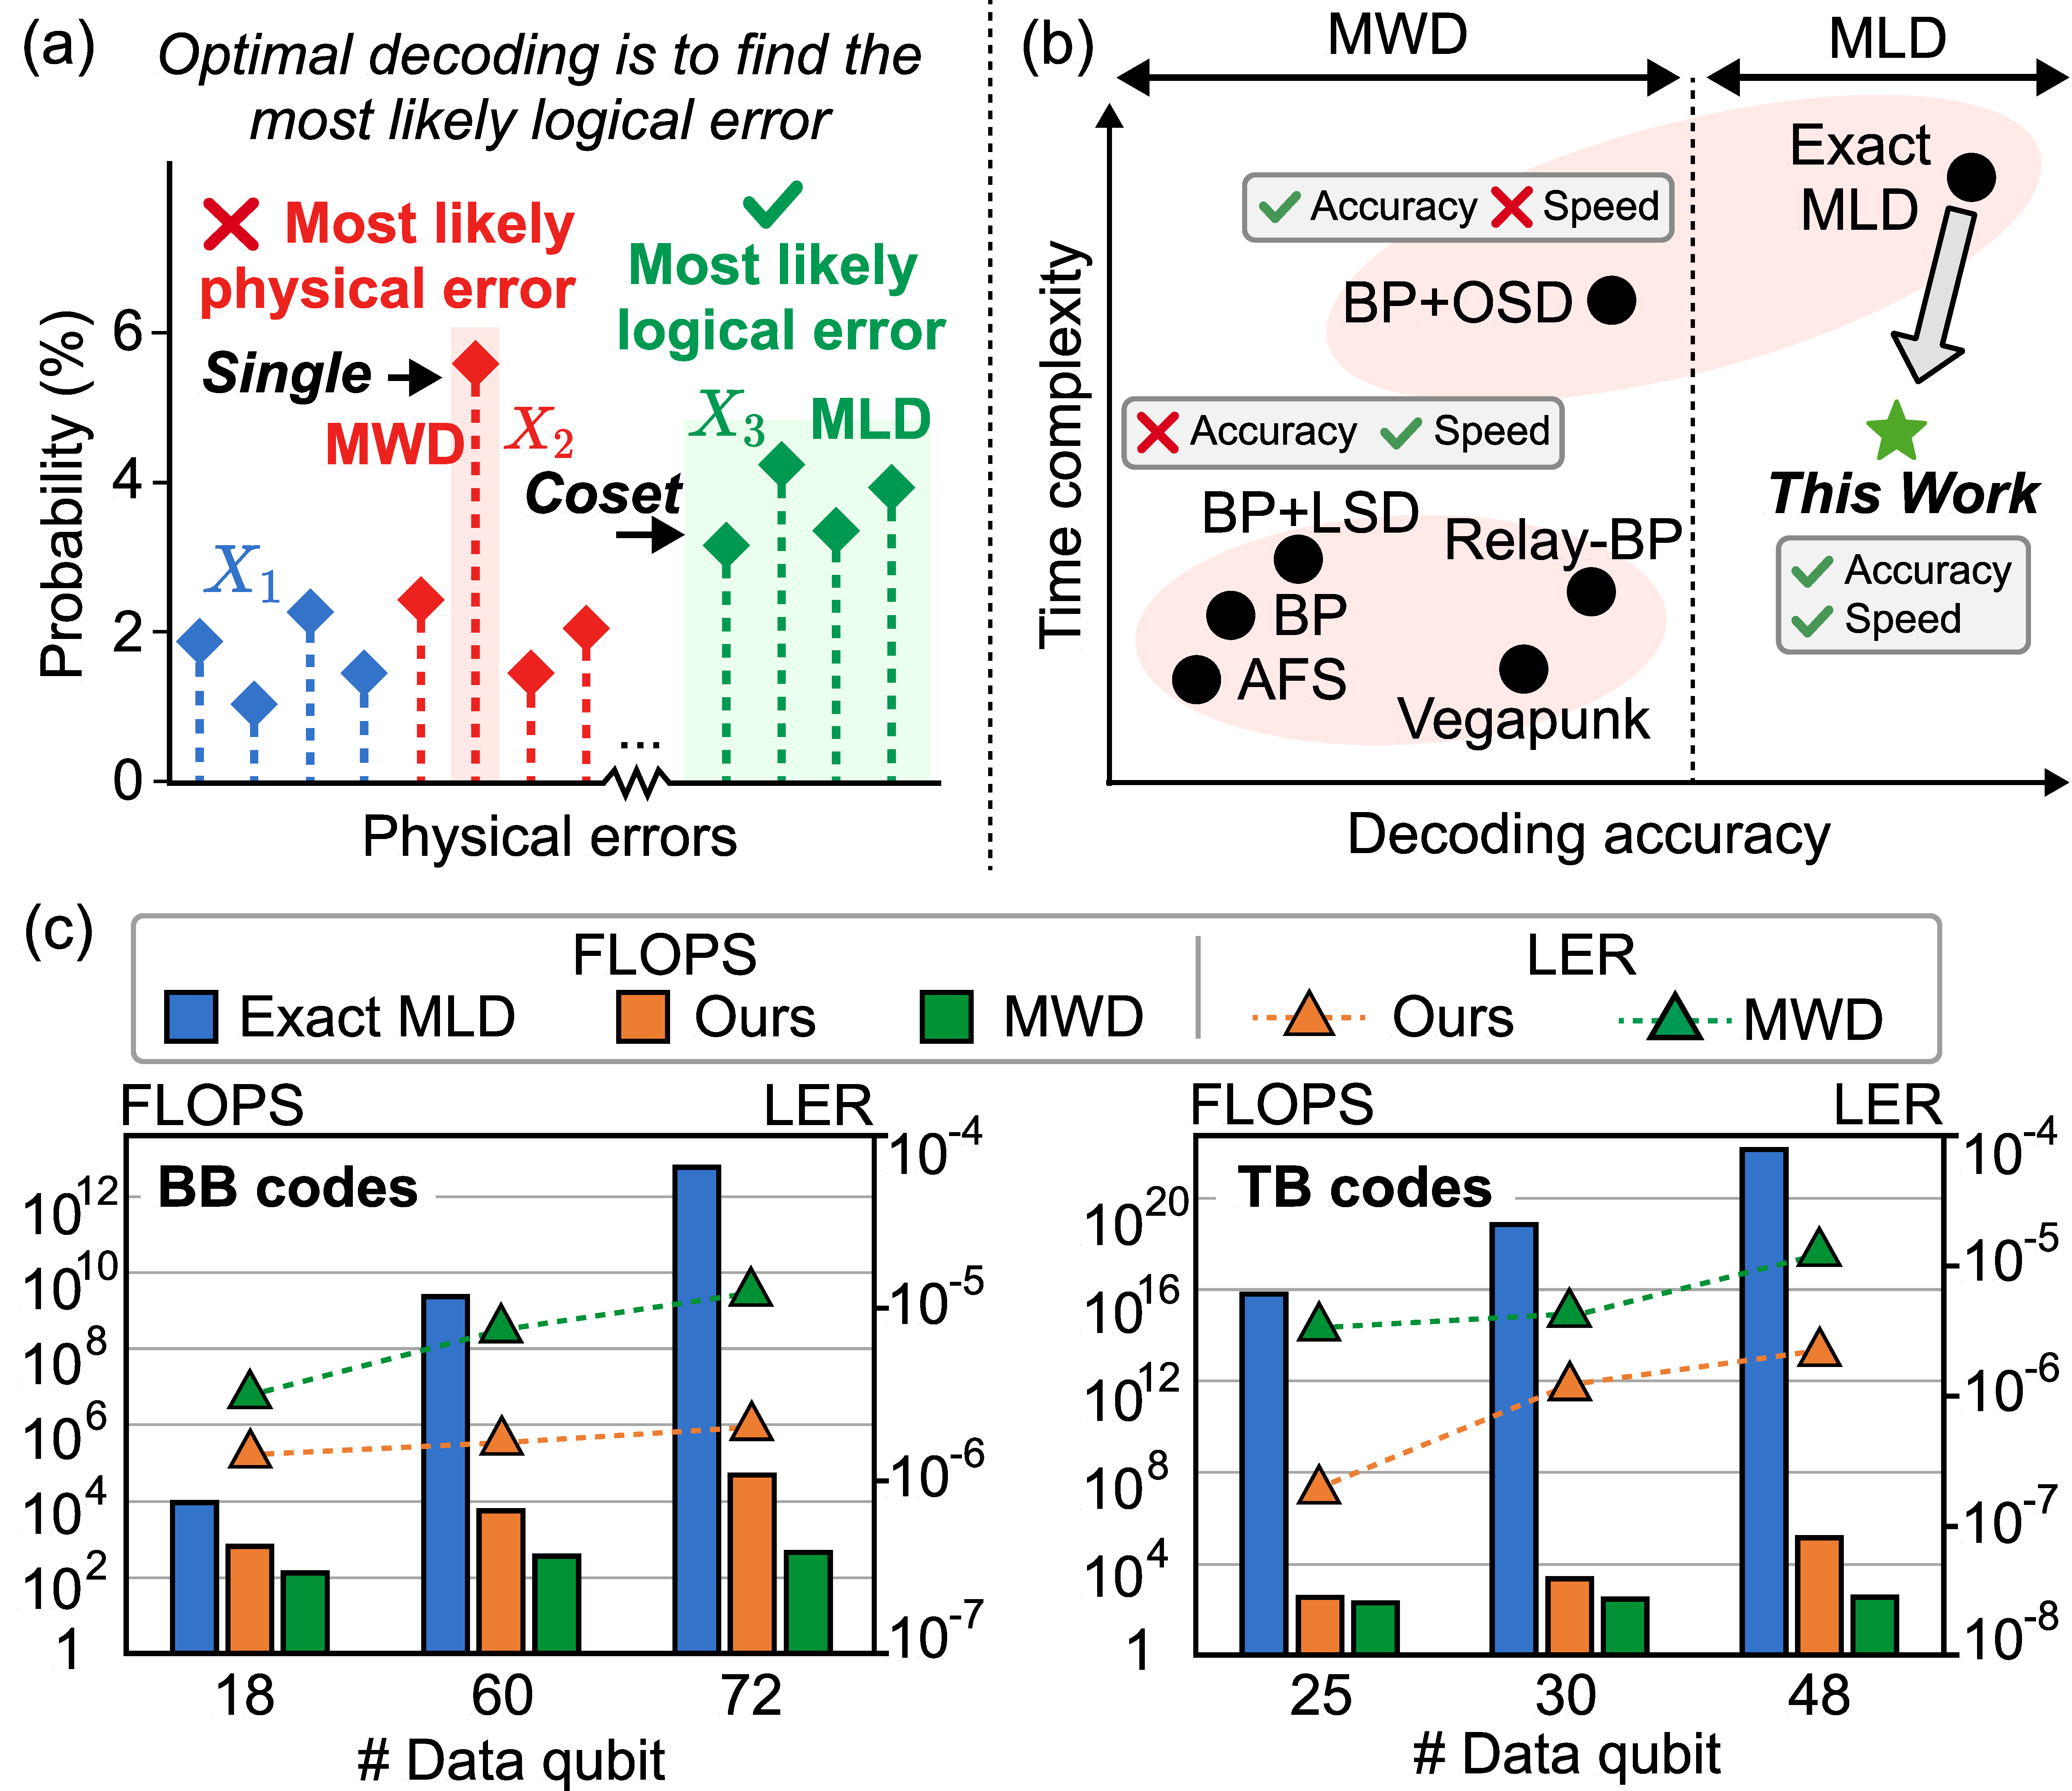
\includegraphics[width=1.0\columnwidth]{figures/intro.pdf}}
\vspace{-0.3cm}
\caption{(a) Difference between minimum weight decoding (MWD) and maximum likelihood decoding (MLD). MLD is optimal since it targets the most likely logical errors.
(b) Trade-off between decoding accuracy and time complexity of existing QEC decoders. They either have low accuracy or high time complexity.
(c) Computational cost (FLOPS) and logical error rate (LER) comparison among exact MLD, \papername, and MWD (BP+OSD) decoder.
} 
\label{fig:intro}
\end{figure}
%%%%%%%%%%%%%%%%%%%%%%%%%%%%%%%%%%%%%%%%%%



%%%%%%%%%%%%%%%%%%%%%%%%%%%%%%%%%%%%%%%%%%
% \begin{table}[t]
\centering
\renewcommand{\arraystretch}{1.2}
\caption{Comparison with other qLDPC decoders.}
\label{tab:intro_comparison}
\resizebox{\linewidth}{!}{
\begin{minipage}{\linewidth}
\begin{tabular}{|l|c|c|c|c|}
\toprule[1pt]
    \textbf{\makecell{Decoder Type}} & \textbf{\makecell{Decoding\\Accuracy}} & \textbf{\makecell{Time\\Complexity}} & \textbf{\makecell{Technical\\Feature}} & \textbf{Principle} \\
    \hline
    AFS \cite{das2022afs} & \bad & \good & \makecell{Union-find} & MWD \\
    \hline
    Astrea \cite{vittal2023astrea} & \good & \medium & \makecell{Graph\\Matching}  & MWD \\
    \hline
    BP \cite{bp} & \bad & \good & \makecell{Message\\Passing}  & MWD \\
    \hline
    BP+OSD \cite{bposd} & \good & \bad & \makecell{Gaussian\\Elimination}  & MWD \\
    \hline
    BP+LSD \cite{bplsd} & \medium & \medium & \makecell{Matrix\\Factorization}  & MWD \\
    \hline
    \textbf{\papername} & \good & \good & \makecell{Tensor\\Compression} & \textbf{MLD} \\
\bottomrule[1pt]
\end{tabular}

\vspace{0.15cm}
\raggedright
\footnotesize
$^*$MWD refers to Minimum Weight Decoding, while MLD means Maximum Likelihood Decoding. \\
$^*$The symbol $\odot$ indicates a medium level.
\end{minipage}
}
\vspace{-0.4cm}
\end{table}


%%%%%%%%%%%%%%%%%%%%%%%%%%%%%%%%%%%%%%%%%%

% 第三段
The design of a qLDPC decoder depends heavily on the target error model, which is typically categorized into \textit{the most likely physical error} and \textit{the most likely logical error}. The former is addressed by minimum-weight decoding (MWD), which selects the physical error with the lowest weight that is consistent with the syndrome. As shown in \autoref{fig:intro}~(a), MWD returns only a single most probable physical error ($\mathbf{X}_2$). In contrast, maximum-likelihood decoding (MLD) evaluates all physical errors within a coset and identifies the most probable logical error ($\mathbf{X}_3$), achieving globally optimal performance~\cite{sundaresan2023demonstrating,mld,jung2020quantum}. Due to quantum degeneracy, the true logical error corresponds to a large set of physical errors, making MWD inherently approximate and often inaccurate. In our experiments, even the state-of-the-art BP+OSD decoder~\cite{bposd} correctly compensates the true logical error with only 18.4\% probability on a 72-qubit bivariate bicycle (BB) code.

% The qLDPC decoder design highly depends on the target error type, which is generally categorized into \textit{the most likely physical error} and \textit{the most likely logical error}. The first one is followed by the minimum weight decoding algorithm (MWD) that minimizes the Hamming weight of the physical error vector while matching the observed syndrome. As illustrated in \autoref{fig:intro}~(a), MWD only identifies one single physical error with the highest probability ($\mathbf{X}_2$). In contrast, the maximum likelihood decoding algorithm (MLD) checks all physical errors and targets the most likely logical error ($\mathbf{X}_3$), achieving globally optimal decoding performance~\cite{sundaresan2023demonstrating,mld,jung2020quantum}. 
% Note that the presence of quantum degeneracy means that the true logical error corresponds to a large coset of possible physical errors. Consequently, the MWD algorithm fundamentally is an approximation of the error information, which may lead to an inaccurate solution. In our experiment, even using the state-of-the-art BP+OSD decoder~\cite{bposd}, the decoded correction has only {18.4\%} probability to compensate for the true logical error in a 72-size bivariate bicycle (BB) code.

% \hl{xxx, qLDPC example of degeneracy}.

% MLD is a higher-level, more complex process that correctly accounts for quantum degeneracy by considering the entire distribution of physical errors that match a given syndrome.
% MLD is to find the logical error whose physical error probability summation is the largest, such as the logical error $X_3$ in \autoref{fig:intro}~(b).
% To be concrete, 
% % \hl{two sentences to explain the flow of MaxLD computation}. 
% \hl{MLD culmulates all probabilities of physical errors that belong to the same logical error, and then selects the logical operator with the most significant probability.}

% generally follow two main principles: Minimum Weight Decoding (MWD) and Maximum Likelihood Decoding (MLD) \cite{gnd,cao2023qecgpt}. MWD aims to find the most likely physical error (often the one with the lowest weight) that matches the observed syndrome. While computationally simpler, MWD is suboptimal. This is because quantum codes exhibit degeneracy, where multiple distinct physical errors can map to the same logical state. In contrast, MLD targets the most probable logical error, achieving optimal decoding performance by considering all possible physical errors within the same logical coset \cite{sundaresan2023demonstrating,mld,jung2020quantum}. 



% For surface codes, MLD-based decoders have achieved linear-time decoding with near-optimal accuracy \cite{bravyi2014efficient}. However, extending MLD to qLDPC codes remains challenging due to the hypergraph structure and high combinatorial complexity, which render exact MLD decoding NP-hard \cite{fujiwara2024quantum}. Consequently, the search space for logical errors grows exponentially with the code size, making scalable MLD for qLDPC codes an open research problem.

% 第四段
Achieving fault-tolerant quantum computing requires low-latency error-correction feedback, which forces decoders to balance accuracy and computational cost. Decoding qLDPC codes is particularly challenging compared with surface codes \cite{bpgdg,wolanski2024ambiguity,maan2025machine,ninkovic2024decoding,yin2024symbreak}, as surface codes have regular 2D locality while qLDPC codes feature irregular hypergraphs with non-local stabilizers. \autoref{fig:intro}~(b) illustrates recent progress in improving the performance of decoding qLDPC codes. We can observe that most studies focus on the MWD principle because MWD inherently approximates the decoding problem to finding a single, most likely physical error, which is computationally more tractable than estimating logical error coset probability with MLD. 
Within the MWD framework, several works aim to achieve higher accuracy~\cite{bposd,muller2025improved}, while others seek to reduce decoding latency~\cite{bplsd,zhou2025vegapunk,yin2024symbreak}. For example, relay-BP improves the accuracy by running BP under different disordered memory strengths~\cite{muller2025improved}, and Vegapunk reduces the latency via guessing the physical error vector in parallel from the decoupled check matrices~\cite{zhou2025vegapunk}. On the other hand, studies of the MLD principle mainly concentrate on arithmetical analysis, and the acceleration is less explored. Specifically, these works often focus on developing algebraic or statistical bounds for the logical error rate~\cite{chubb2021statistical,
xu2024constant,jung2020quantum}. 
For example, Chubb et.al. give the exact threshold of the surface code under mildly correlated bit-flip noise~\cite{chubb2021statistical}.



% \hl{MLD inherently has a higher fault-tolerance threshold than MWD, which means the error in the quantum chip can be corrected by the same code distance, even with higher error rates. Thus, MLD can 
% Besides, MLD also reduces the logical error rates of the qLDPC codes with simpler topology connections, making }
% % %MLD 对比 MWD 优势
% \hl{Therefore, an accuracy-complexity co-design is strongly desired, which is essential for accurate and fast evaluation for different QEC codes, as the development of quantum chips.}

% where several works aim to achieve higher accuracy~\cite{bposd}, while others seek to reduce decoding latency~\cite{bplsd,zhou2025vegapunk,yin2024symbreak}. We can observe that most studies focus on the MWD principle because \hl{MWD inherently approximates the decoding problem to finding a single, most likely physical error, which is computationally much more tractable than estimating logical error rates}. On the other hand, the MLD principle is less explored due to \hl{its fundamentally greater computational complexity, as it requires summing the total probability of all possible physical errors belonging to the same logical errors.}~\cite{jung2020quantum}. 

% 目前对于MLD的研究更多停留在理论层面，试图xxx。例如，xxx

%我们的目标是在不降低MLD的精度的前提下，如何尽可能的降低time complexity. 然后结合MLD的计算本质讲一下challenge。然后讲为什么MWD的方法不能直接迁移过来。给些example，例如用xxx MWD加速方法，MLD精度会降多少。In a word，当前缺乏面向MLD的accuracy-complexity co-optimization的工作。



% Currently, research into MLD is largely theoretical, attempting to establish the theoretical limits and optimal performance of quantum error correction by defining the true minimum logical error rate. For instance, theoretical work often focuses on developing algebraic or statistical bounds for the logical error rate without proposing practical, high-speed implementations~\cite{xu2024constant}. 

Compared to MWD, MLD inherently delivers a higher fault-tolerance threshold, allowing for higher noise levels in the future design of large-scale quantum chips. Furthermore, a low logical error rate also helps to simplify the connectivity among qubits~\cite{cao2025exact,chubb2021statistical}, making the chip less sensitive to the technology.
Mathematically, the MLD calculates the logical probability by accumulating all probabilities
of physical errors that belong to the same logical error~\cite{jung2020quantum}. And then, it identifies the largest logical probability among all possible logical errors. {This enlarges the computation workload of MLD, causing a higher FLOPS compared with MWD, as shown in }\autoref{fig:intro}~(c).
%除了accumulate，还要做啥复杂计算。
However, the computation flow of MLD is entirely different from that of MWD, making existing MWD optimizations ineffective for accelerating MLD. For example, applying the early-termination~\cite{das2022afs} or hardware-pruning~\cite{alavisamani2024promatch,zhou2025vegapunk} MWD accelerator to the MLD decoder will severely damage the fidelity (e.g., logical error rate increases from $10^{-6}$ to $10^{-4}$), due to the inaccurate truncation of the critical probability summation. \textit{In a word, an accuracy-complexity MLD co-design is strongly desired, which can inherit its accuracy advantage meanwhile tackling the overwhelming computational pressure}. 

% Our goal is to minimize the time complexity of MLD without compromising its superior accuracy. The core challenge lies in the computational nature of MLD itself: it needs to accumulate all probabilities
% of physical errors that belong to the same logical error~\cite{jung2020quantum}. This is fundamentally different from the MWD computation, which is an optimization problem seeking the single minimum-weight (most-probable) physical error.
% Consequently, MWD acceleration methods cannot be directly migrated to MLD. For example, applying a simple early-termination or hardware-pruning MWD acceleration method to an MLD decoder would directly lead to an inaccurate truncation of the crucial probability summation, significantly degrading the MLD accuracy, potentially by several orders of magnitude (e.g., from $10^{-6}$ to $10^{-4}$).
% % Forcing an MWD-based accelerator to perform MLD probability summation would dramatically increase latency and make the decoder completely useless for real-time operation.
% In a word, there is a current lack of work dedicated to the accuracy-complexity co-optimization specifically for MLD, leaving its high-accuracy potential untapped in practical, low-latency quantum computing systems.

% Current practical decoders are all based on the MWD principles, \textit{focusing on the trade-off between accuracy and time complexity,} as illustrated in \autoref{fig: intro}~(a). This focus is necessary because decoding qLDPC codes is significantly more challenging than decoding surface codes \cite{bpgdg,wolanski2024ambiguity,maan2025machine,ninkovic2024decoding,yin2024symbreak}. Surface codes benefit from a regular 2D lattice structure and local stabilizer interactions. This simple structure allows for highly efficient MWD decoders like AFS \cite{das2022afs} (based on union-find) and Astrea \cite{vittal2023astrea} (based on graph matching), which effectively solve the accuracy-complexity trade-off. In contrast, qLDPC codes are defined over irregular hypergraphs with non-local interactions, a structure that makes these surface code decoder solutions invalid\cite{zhu2025topological,zhou2025vegapunk,eberhardt2024pruning}. The most commonly adopted decoders for qLDPC codes are based on Belief Propagation (BP)~\cite{bp}. Standard BP uses iterative message-passing, which is fast, but its accuracy is limited by degeneracy \cite{yin2024symbreak,kuo2022exploiting,bpgd}. To improve accuracy, BP with Ordered Statistics Decoding (BP+OSD) \cite{bposd} performs complex post-processing to explore low-weight error subsets, achieving higher accuracy at the cost of high time complexity. Conversely, BP with Localized Statistics Decoding (BP+LSD) \cite{bplsd} aims for an accuracy-complexity balance, using parallel matrix factorization to achieve medium accuracy and complexity. 
% As \autoref{tab:intro_comparison} suggests, these MWD-based decoders represent different points on the accuracy-complexity domain.



% For the optimal MLD decoders, work has been largely theoretical, with \textit{no practical, high-speed decoder or accelerator available to achieve the accuracy-complexity trade-offs.}
% Applying the MLD principle in existing MWD-based decoders or hardware accelerators is non-trivial. These systems are fundamentally designed for the MWD principle: to find a single, most-probable physical error pattern. In contrast, the MLD principle requires a fundamentally different and more complex computation: estimating the total probability of all possible logical errors 
% ~\cite{jung2020quantum}. Forcing an MWD-based architecture to perform this probability summation would dramatically increase latency and make the decoder completely useless for real-time operation.


In this paper, we propose \papername, the first MLD decoder design that systematically balances the accuracy and time complexity. Our key novelty lies in the tensorization and compression for the decoding process for the most likely logical error. Considering that MLD is globally disordered with 0 or 1 values, we map the decoding problem into a spin-glass model~\cite{jaddi2020ldpc,kovalev2015spin}, which can then be computed through the tensor network~\cite {orus2019tensor,montangero2018introduction}. However, this raw tensor network still exhibits $2^n$ complexity, resulting in a significant computation cost and memory bottleneck. Thus, we then propose an exact tensor decomposition scheme that shrinks the original $O(2^n)$ tensor to a matrix product state (MPS) with a linear complexity of $O(8n)$, e.g., from 3.9GB to 8.7KB for 254-size trivariate bicycle codes. Furthermore, we flatten the high-dimensional connection in MPS into a 1D chain and successfully compress the computation requirement from TFLOPS-level to KFLOPS-level.

Next, we present our online decoding flow and hardware accelerator architecture. 
% \hl{xxx}
% its ability to precisely calculate logical error probabilities by mapping the decoding problem into a spin-glass model~\cite{jaddi2020ldpc,kovalev2015spin}
While the 1D chain MPS encodes all logical error probability information, directly enumerating all logical errors still incurs an exponential computational cost. To address this issue, we develop a partial tracing strategy to compute the conditional marginal probability of each logical spin in parallel. This approach maintains decoding accuracy while reducing the time complexity to polynomial time related to the number of logical qubits. Finally, we implement this efficient decoding flow on a GPU device through a dedicated hardware architecture, which leverages Tensor cores for matrix product operations and CUDA cores for calculating marginal logical probabilities.

% The key novelty of \papername lies in its ability to precisely calculate logical error probabilities by mapping the decoding problem into a spin-glass model~\cite{jaddi2020ldpc,kovalev2015spin}, 
% % 由于decoding和spin-glass model都呈现什么样的数据特性，我们选择map过去并用xx方法加速求解xxxx
% which can then be efficiently computed via the tensor network~\cite {orus2019tensor,montangero2018introduction}.
% However, the direct tensorization yields a tensor network composed of many high-rank tensors, inherently demanding exponential storage space and computational cost. For example, the memory footprint of 180-qubit trivariate bicycle codes exceeds 3 GB, and the computation overhead of 72-qubit BB codes is 6.07 TFLOPS.

% To address these challenges, we present three optimization passes to compress the tensor network.
% First, to solve the storage bottleneck, we introduce an exact decomposition of these high-rank tensors into a linear number of low-rank Matrix Product States (MPS)~\cite{orus2014practical}, achieving a reduction in storage space from exponential to linear complexity. Though this addresses the storage issue, the high-dimensional topological connections inherent in the MPS structure still contribute to substantial computational overhead. To handle this, we design an offline contraction method that systematically approximates the high-dimensional topologically connected MPS into a one-dimensional (1D) chain MPS.
% Crucially, this 1D chain MPS can be contracted in linear time, enabling efficient online decoding. \hl{This heavily reduce the computation cost of MLD by over $10^8\times$ and achieve a similar level with MWD,} \hl{as shown in} \autoref{fig:intro}~(c).
% Finally, while the 1D chain MPS encodes all logical error probability information, directly enumerating all logical errors still incurs an exponential computational cost. To further reduce the complexity of online decoding, we propose to compute the marginal probabilities in parallel, conditioned on highly probable logical spins. By leveraging marginal probability to determine the most likely logical qubit, we achieve a robust and accurate estimate of the most likely logical error in polynomial time to the number of logical qubits. \autoref{fig:intro}~(c) depcits that \hl{our decoding method achieve $2.5\times\sim 16.7\times$ LER reduction over MLD across all codes.}

Our contributions are summarized as follows:
\begin{itemize}
\item Targeting the most likely logical error, \papername is the first work that tries to balance the decoding accuracy and time complexity. Inspired by the spin glass model, we tensorize the decoding flow into the computation of high-rank tensors, exposing the opportunity for parallelism
\item We propose two compression techniques: exact tensor decomposition and offline tensor contraction, which greatly cut down the computational cost while exhibiting little accuracy loss. 
\item We propose the overall decoding flow with an efficient hardware accelerator. We employ a conditional marginal probability strategy to achieve polynomial-time complexity, equipped with GPU accelerator.
\end{itemize}

% 还要讲相比于传统MLD降低了多少FLOPS，多少memory requirement，在A100上的时间是多少
% \hl{xxx}
Experimental results demonstrate that \papername achieves the lowest logical error rate, which is $1.55\sim112\times$ lower than the state-of-the-art BP+OSD decoder. 
% \papername also improves the fault-tolerant threshold from 1.61\% to 1.76\% on BB codes, from 1.53\% to 1.60\% on trivariate bicycle codes, compared with BP+OSD. 
\papername achieves this MLD-level accuracy while reducing max tensor size by $8.0\sim 10^{16}\times$ and computational workload by $14.2\sim 10^{17}\times$, compared with the original MLD tensor network decoder. Concretely, \papername compresses the memory footprint from  3.9GB to 8.7KB in 254-size bivariate bicycle codes and reduces the computation workload from $10^7$PFLOPS to 131KFPLOS in 48-size bivariate bicycle codes.
\section{Background}



\subsection{Basics of qLDPC codes}
Quantum low-density parity-check (qLDPC) codes are a class of quantum error-correcting codes defined by two sparse binary parity-check matrices $H_{X}$ and $H_{Z}$, which satisfy the commutation constraint $H_{X}H_{Z}^{T}=0$. These two matrices describe the stabilizer that detects errors, where $H_{X}$ corresponds to phase ($Z$) errors and $H_{Z}$ relates to bit-flip ($X$) errors, respectively. As shown in \autoref{fig:background} (a), the structure of qLDPC codes can be represented by a Tanner graph. It is a bipartite graph that connects data qubits to parity checks, where the edges stem from the non-zero entries in $H_{X}$ and $H_{Z}$. Measuring the parity check qubits will give the syndrome that encodes the error types and locations.

Unlike surface codes, where the decoding problem reduces to finding minimum-weight perfect matchings on a planar graph \cite{wu2023fusion,vittal2023astrea}, qLDPC codes generally induce a hypergraph structure due to the complex connectivity and the higher weight of stabilizers \cite{berlekamp2003inherent}. Each stabilizer can involve a logarithmic or constant number of qubits with non-local interactions, resulting in dense and irregular Tanner graphs. This hypergraph topology leads to an NP-hard decoding problem, where the ideal objective is to infer the most probable logical error given a syndrome \cite{iyer2015hardness}.

\begin{figure}[t]
\centerline{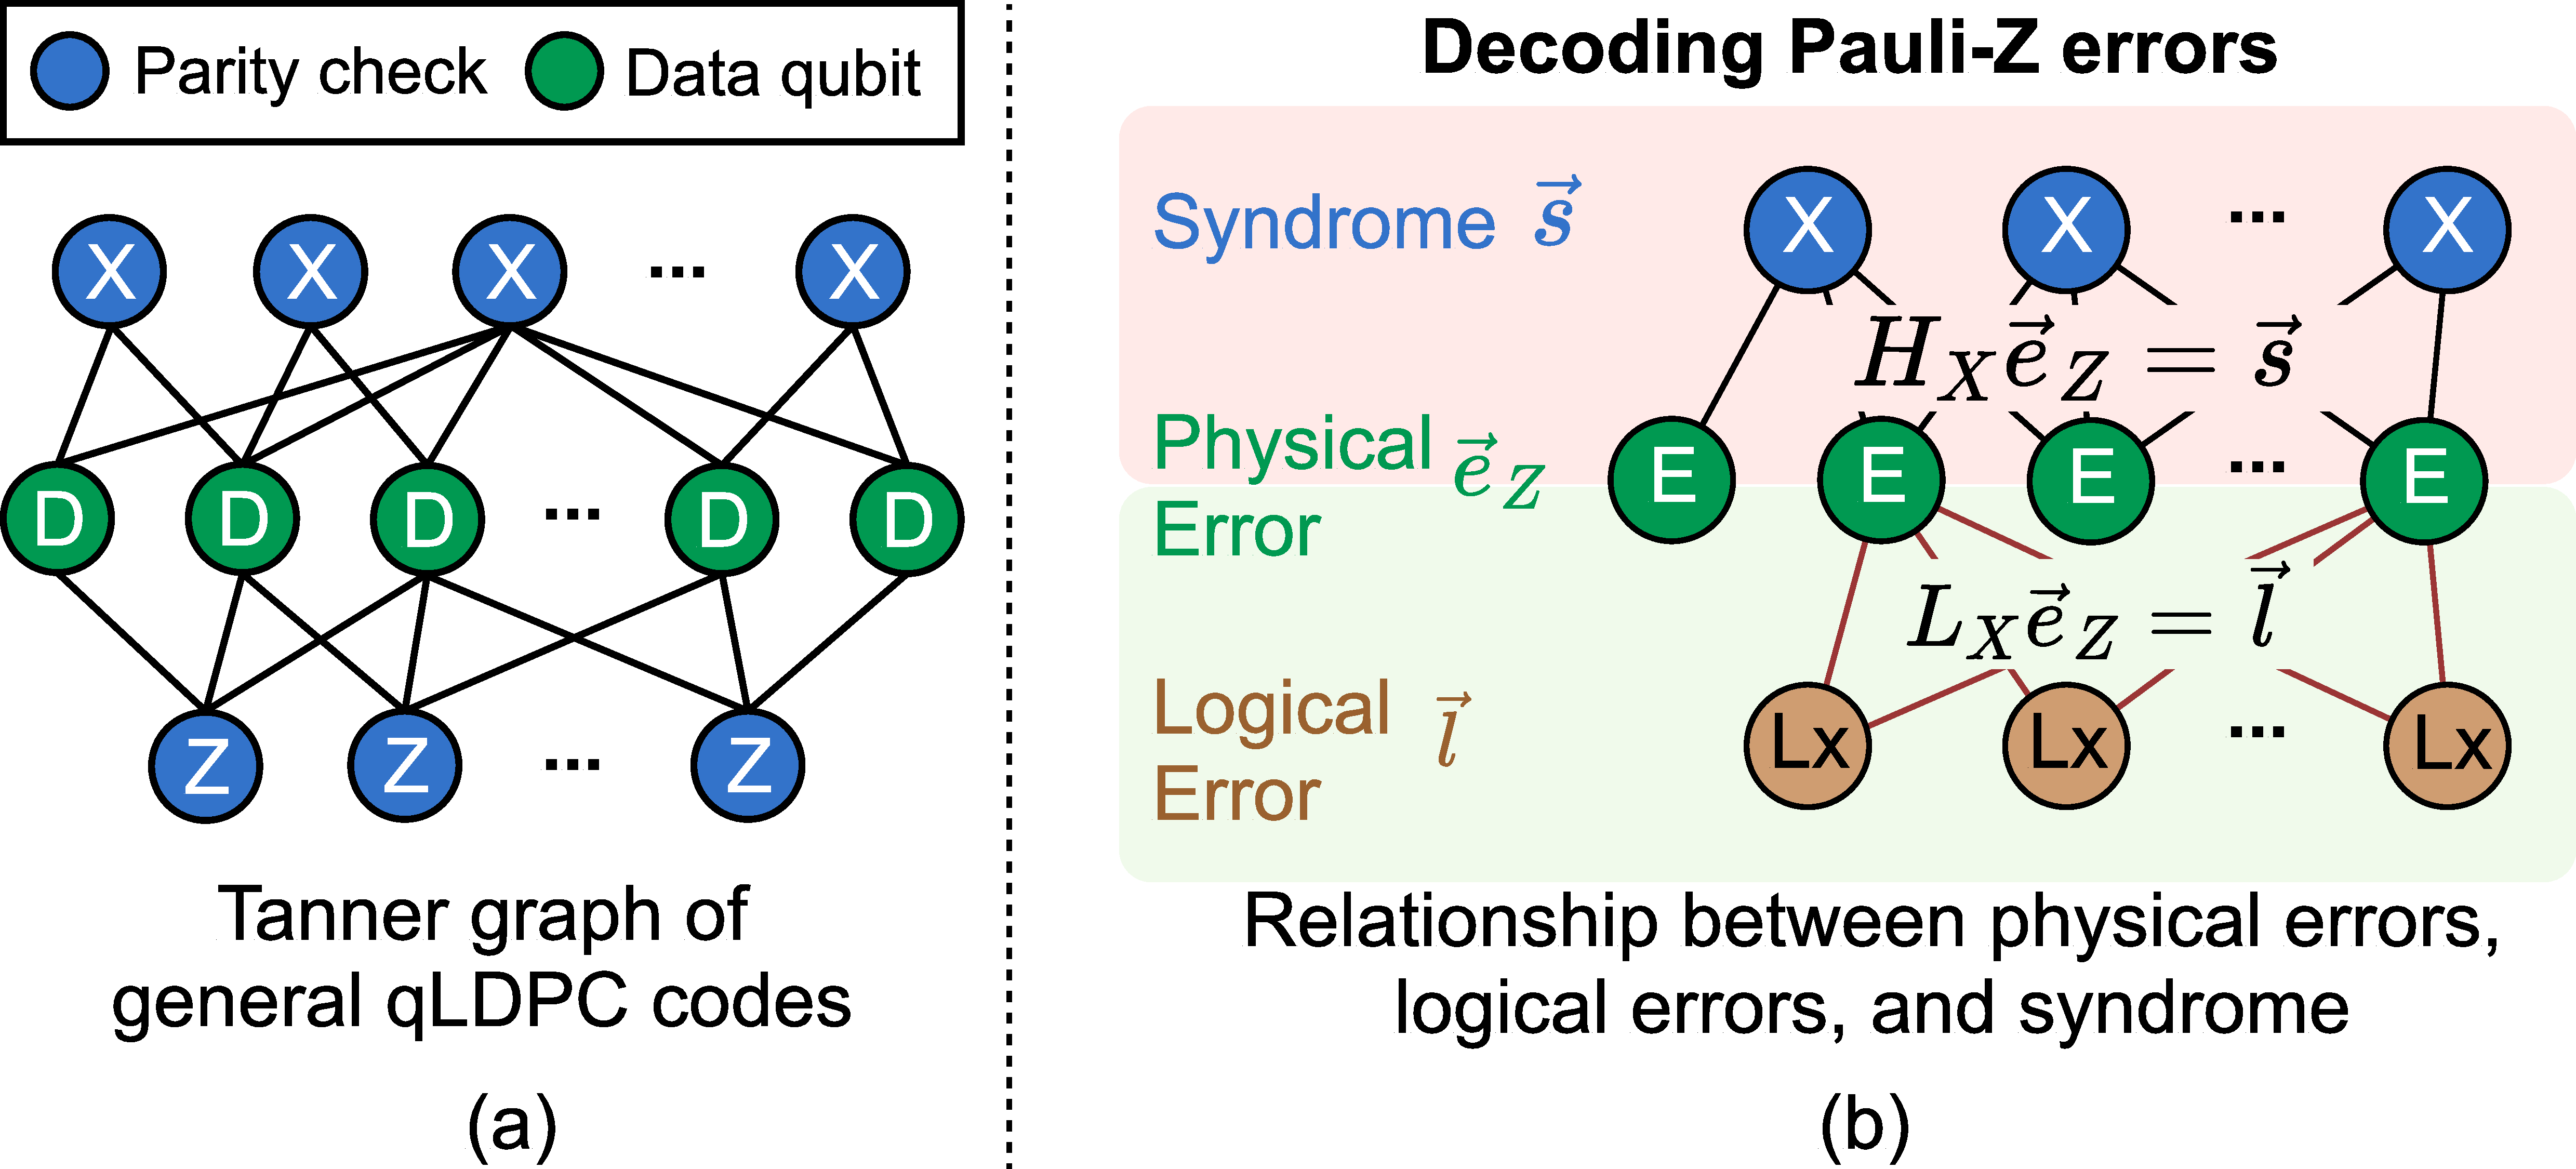
\includegraphics[width=1.0\columnwidth]{figures/background.pdf}}
\vspace{-0.4cm}
\caption{(a) Tanner graph of general qLDPC codes. (b) The relationship between physical errors,
logical errors, and syndrome. 
% (c) Illustration of BP and BP+OSD decoder. If BP fails to converge, it triggers the OSD part as post-processing.
} 
\vspace{-0.4cm}
\label{fig:background}
\end{figure}

\subsection{MLD Decoding}
% Decoding qLDPC codes requires a realistic noise model that reflects the behavior of actual quantum hardware. Simplified models (e.g., independent bit-flip) ignore the temporal and spatial correlations introduced by faulty quantum circuits. In contrast, the circuit-level depolarizing noise model accounts for errors during all elementary operations in the syndrome measurement circuit, including gate faults, qubit initialization and measurement errors, and idle decoherence. Each operation is assumed to fail independently with probability $p$, and upon failure, a uniformly random nontrivial Pauli error ($X$, $Y$, or $Z$) is applied to the affected qubit(s), consistent with a depolarizing channel. These errors may then propagate through the circuit, creating complex correlated error patterns that the decoder must properly handle.
Noise on the qLDPC codes circuit can be described as a physical error vector $\vec{e}$, where $e_j=1$ means an error occurs in the $j$-th position, while $e_j=0$ means no error in this position.
The physical errors can be decomposed into Pauli-X errors and Pauli-Z errors, which eventually cause the logical Pauli-X or Pauli-Z errors on logical qubits. Thus, the decoding objective of QLDPC is to infer the logical errors and correct the logical qubits. Since qLDPC codes belong to CSS codes, the Pauli-X and Pauli-Z errors can be decoded independently~\cite{bposd}. Without loss of generality, we focus on the decoding of Pauli-Z errors.

To detect the Pauli-Z errors $\vec{e}_Z$, measurements are applied on the X-type parity check qubits to give the syndrome vectors $\vec{s}$. 
As shown in \autoref{fig:background}~(b), the relationship between physical error $\vec{e}_Z$, logical error $\vec{l}$, and syndrome $\vec{s}$ can be expressed as
\begin{equation}\small\label{eq:decodingrelation}
    \begin{bmatrix} 
H_X \\ L_X
\end{bmatrix} \vec{e_Z} = \begin{bmatrix}
\vec{s} \\ \vec{l}
\end{bmatrix} \mod 2 \;.
\end{equation}
Here, $H_X$ is the parity check matrix, where each row is an X-stabilizer. $L_X$ is the logical check matrix, where each row is an X logical operator. 
% \autoref{fig:ablation_study}~(b) also shows the decoding relationship of Pauli-X errors and the commutation relationship between decoding Pauli-X and Pauli-Z errors.

% To decode under a circuit-level depolarizing noise model, a check matrix $H$ needs to be constructed, which maps circuit faults to measured syndromes across multiple rounds. \autoref{fig:background} (b) illustrates the syndrome measurement circuit of Bivariate Bicycle (BB) codes \cite{bbcode}, where parity checks interact with data qubits through CNOT gates and are measured to extract syndromes. Errors on CNOT gates, parity checks, or data qubits can propagate and affect the measured outcomes. For CSS-type qLDPC codes, $X$ and $Z$ errors can be decoded separately, allowing the construction of two independent decoding matrices $H_x$ and $H_z$. By unrolling the circuit over $d$ consecutive rounds, each column of $H_x$ or $H_z$ represents a fault event at a specific space-time location, and each row corresponds to a syndrome bit at a given round. As the number of measurement rounds increases, the decoding matrix grows vertically (more syndrome bits) and horizontally (more fault events), forming a temporally extended representation of the full decoding problem.



% \subsection{MLD decoding}

The maximum likelihood decoding (MLD) for qLDPC codes centers on finding the most 
likely logical error \( \vec{l}^* \) given an observed syndrome \( \vec{s} \), following \eqref{eq:decodingrelation}.
Here, we use Pauli-Z errors $\vec{e}_Z=\{e_1,e_2,\cdots,e_j,\cdots\}$ for illustration, where each error \( e_j \in \{0,1\} \) has physical error probability \( p_j \). The goal is to maximize the logical probability $P(\vec{l}|\vec{s})$ under a given syndrome $\vec{s}$,
\begin{equation}\small
\vec{l}^* = \arg\max_{\vec{l}} P(\vec{l}|\vec{s}).
\label{eq:logicalsyndrome}
\end{equation}
Here, the logical probability $P(\vec{l}|\vec{s})$ is calculated by accumulating all physical errors $\vec{e}_Z$ that belong to the logical error $\vec{l}$ and match the syndrome $\vec{s}$,
\begin{equation}\small \label{eq:logicalprobcons}
    P(\vec{l}|\vec{s}) = \sum_{\{\vec{e}_Z \mid 
H_X \vec{e}_Z = \vec{s}, L_X\vec{e}_Z  =\vec{l} \}} P(\vec{e}_Z) 
\end{equation}

\begin{equation}\small
P(\vec{e}_Z) = e^{-\sum_{j=1}^n 2w_j e_j}, \quad w_j = \ln \left( (1 - p_j)/p_j \right) /2 \label{eq:errorrate}
\end{equation}
where \( P(\vec{e}_Z)  \) is the physical error probability and $p_j$ is the phyiscal probability of occuring $j$-th error, \ie, $e_j=1$. $w_j$ is called error weight of $j$-th error.
After dedecting the moskly logical errors $\vec{l}^*$, the detected logical operator for error correction is,
\begin{equation} \small
    \hat{L} = H_{\text{des}}^T \vec{s} \oplus L_X^T \vec{l}^* \label{eq:recovererror}
\end{equation}
where $H_{\text{des}}$ is the matrix with each row a Z-destabilizer. 
% Since \eqref{eq:recovererror} is a deterministic process, the goal of maximum likelihood is to find the most likely logical errors in \eqref{eq:logicalsyndrome}.

% MWD decoders aim to identify the most probable physical error consistent with the observed syndrome. This formulation offers relatively low computational complexity, which makes these decoders practical for near-term implementations. However, it also inherently limits their decoding accuracy. As illustrated in the red bar of \autoref{fig:motivation}~(a), MWD focuses on recovering the most likely physical error, whereas the true objective of quantum error correction is to recover the most probable logical state (i.e., to identify the most likely logical coset), shown in the green region. Because qLDPC codes exhibit high \textit{quantum degeneracy}, multiple distinct physical errors can correspond to the same logical error. Consequently, the most likely physical error may reside in an incorrect logical coset, leading to logical failures even when the physical correction appears optimal \cite{gnd,cao2023qecgpt}. Therefore, while MWD decoders offer efficiency, their accuracy remains fundamentally suboptimal.

% For computational efficiency, we express this as:
% \[\small
% P(\vec{e}_Z) = e^{-\sum_{j=1}^n 2w_j e_j}, \quad w_j = \ln \left( (1 - p_j)/p_j \right) /2
% \]

% \subsection{BP and BP+OSD Decoder}
% The most widely used decoders for qLDPC codes are Belief Propagation (BP) \cite{bp} and Belief Propagation with Ordered Statistics Decoding (BP+OSD) \cite{bposd}, as shown in \autoref{fig:background}~(c).
% BP is an iterative probabilistic decoding algorithm that operates on the Tanner graph of the code, where messages representing error probabilities are exchanged between variable nodes (data qubits) and check nodes (parity checks). Through successive iterations, BP updates these messages based on the syndrome and the graph’s connectivity, gradually refining the posterior probabilities of qubit errors. However, in quantum codes, the presence of quantum degeneracy, where multiple distinct error patterns produce the same syndrome, can cause BP to converge to an incorrect solution.

% To address this limitation, the OSD technique is often integrated with BP as a post-process, forming the BP+OSD decoder. In this hybrid approach, BP is first used to estimate the error probabilities of data qubits. Then, OSD reorders the columns of the parity-check matrix according to these probabilities and applies Gaussian elimination to extract a set of linearly independent columns, transforming the matrix into an invertible form. This allows the decoder to directly compute an error pattern consistent with the syndrome by solving a linear system. By leveraging the probability information provided by BP, OSD corrects for the failures caused by quantum degeneracy and significantly improves decoding accuracy.
% \input{sections/03_motivation}
\section{\papername Tensorization and Compression} \label{sec:formulation}

\begin{figure*}[t]
\centerline{
\includegraphics[width=1\textwidth]{figures/formulation.pdf}}
\vspace{-0.2cm}
\caption{Formulating the (a) maximum likelihood decoding as (b) minimizing the free energy of the spin glass model, and using (c) the tensor network to calculate the free energy.} 
\vspace{-0.4cm}
\label{fig:formulation}
\end{figure*}

To balance the decoding accuracy and computational complexity, we first convert the constrained calculation into an unconstrained summation format. Then, the computation for this summation is tensorized using the spin glass model, where 
the errors and syndromes are converted into spins. After this, the logical probabilities are calculated by the free energies of the spin glass system, which can be efficiently computed by the tensor network.
Although the tensorization exposes the opportunity to parallel the MLD computation, the overall memory footprint and computational workload (FLOPs) still grow exponentially with the qLDPC code size. Identifying that the tensors from the spin glass model can be expressed by a product of constant-dimensional matrices, we propose an exact tensor decomposition that shrinks the original $O(2^n)$ tensor to a matrix product state (MPS) with a linear complexity of $O(8n)$, from 
3.9GB to 8.7KB for 254-size trivariate bicycle codes. To further reduce the computational workload, we flatten the high-dimensional connection in MPS into a 1D chain. We achieve this by swapping the tensor indices and merging adjacent matrices to eliminate high-dimensional connections without loss of logical probability information. Finally, we successfully compress the computation requirement from 6.1 TFLOPS to 48 KFLOPS, with little accuracy loss.



\subsection{Tensorizing MLD with Spin Glass Model}

Calculating the logical error probability with \eqref{eq:logicalprobcons} is non-trivial, as we need to determine the total probability by scanning all physical errors that satisfy two constraints: 1) belong to the same logical error.  2) produce the observed syndrome;
Since checking these two constraints will consume computing resources, we tend to convert the formula into an unconstrained summation format. Clearly, as shown in \autoref{fig:formulation}~(a), we decompose the logical error space $\vec{e}_Z$ into stabilizer subspaces $H_Z^T$ that are shifted by destabilizers $H_{\text{des}}^T$ and logical operators $L_Z^T$,
\begin{equation}\small
    \vec{e}_Z= H_Z^T \vec{z} \oplus H_{des}^T\vec{s}\oplus L_Z^T\vec{l},\forall \vec{z}\in\{0,1\}^M
\end{equation}
Combining this equation with the logical probability $P(\vec{l}|\vec{s})$ in \eqref{eq:logicalprobcons} gives an unconstrained summation over all possible stabilizers $\vec{z}$ as
\begin{equation}\label{eq:logicalstabsummation}
    P(\vec{l}|\vec{s}) =  \textstyle  \sum_{\vec{z} \in \{0,1\}^M} P(H_{\text{des}}^T \vec{s} \oplus H_Z^T \vec{z} \oplus L_Z^T \vec{l})\;.
\end{equation}
The mathematical derivation is summarized in \hyperref[subsec:proofA]{Appendix A}.

However, this summation still has exponential complexity.
To further simplify this, we recast the decoding problem within the framework of the spin glass model, which has broad application in discrete optimization problems~\cite{wiki_spin_glass}. A representative application is that this model is widely used in statistical mechanics to study systems with disorder and frustrated interactions, matching the properties of our formulation. Concretely, the error in decoding problem has two discrete states, 0 or 1, which resemble the two states in the spin glass model, the up(+1) and down(-1) spin rotations. This inspires us to represent stabilizer bits $\vec{z}$, syndrome $\vec{s}$, and logical bits $\vec{l}$ in ~\eqref{eq:logicalstabsummation} as stabilizer spins $\vec{t}$, syndrome spins $\vec{y}$ and logical spins $\vec{g}$ via the bits-to-spin mapping,
\begin{equation}
    (-1)^{z_k} = t_k, ~~(-1)^{s_k} = y_k, ~~(-1)^{l_k} = g_k\;.
\end{equation}
As shown in \autoref{fig:formulation}~(b), mapping bits to spins transforms the probability into the energy of a spin glass determined by the Hamiltonian $H$,
\begin{equation}\small
    H = -\sum_{j=1}^{n} \omega_j\prod_{\{k|H_z(k,j)\neq0\}} t_k  \prod_{\{k|H_{\text{des}}(k,j)\neq0\}} y_k  \prod_{\{k|L_z(k,j)\neq0\}} g_k \;.
\end{equation}
 The logical error probability under the spin glass system is
\begin{equation}\small\label{eq:logicalprobfreeenergy}
    P(\vec{l}|\vec{s})=  \textstyle \sum_{\vec{t}\in\{-1,1\}^{M}} e^{-H}
\end{equation}
The mathematical derivation is summarized in \hyperref[subsec:proofB]{Appendix B}. 

% This equation is related to the free energy $F$ of the spin glass model in statistical mechanics by $F = -\ln P(\vec{l}|\vec{s}) $~\cite{chubb2021statistical}. 
Finally, it has been demonstrated that the spin glass model can be efficiently calculated via a tensor network~\cite{cao2025exact}, exposing the opportunity to tensorize \eqref{eq:logicalprobfreeenergy}. By mapping the energy terms and spin variables in \autoref{fig:formulation}~(b) to the energy tensor $T_j$ and Kronecker Tensor $\delta$, we convert the summation operation in \eqref{eq:logicalprobfreeenergy} into the contraction of the tensor network $\mathcal{T}$ in \autoref{fig:formulation}~(c). As a result, the logical error probability $P(\vec{l}|\vec{s})$ is reformulated as the contraction of the tensor network $\mathcal{T}$. Here is the formal lemma, where the proof can be found in \hyperref[subsec:proofC]{Appendix C}.
\begin{lemma}\label{theorem:decodingTensor}
    The probability of logical error $\vec{l}$ with given syndrome $\vec{s}$, noted as $P(\vec{l}|\vec{s})$, can be calculated via tensor network $\mathcal{T}$ contraction as
    \begin{equation}\small
    P(\vec{l}|\vec{s}) = 
    \frac{{\text{contract}}(\mathcal{T}(\vec{l},\vec{s}))}{\text{contract}(\mathcal{T}(\vec{s}))}. 
    \end{equation}
\end{lemma}

% Since the spin glass model can be efficiently calculated via a tensor network~\cite{cao2025exact}, we thus try to convert \eqref{eq:logicalprobfreeenergy} into tensor computations.
% Through mapping the energy terms and spin variables in \autoref{fig:formulation}~(b) to the energy tensor $T_j$ and Kronecker Tensor $\delta$, we convert the summation operation in \eqref{eq:logicalprobfreeenergy} into the contraction of the tensor network $\mathcal{T}$ in \autoref{fig:formulation}~(c).
% % Typically, the free energy of the spin glass model can be efficiently computed with contraction on the tensor network $\mathcal{T}$ in \autoref{fig:formulation}~(c)~\cite{cao2025exact,chubb2021statistical}.
% Finally, the logical error probability $P(\vec{l}|\vec{s})$ is calculated with the contraction of the tensor network $\mathcal{T}$, as formally stated in the following lemma.


This tensor network $\mathcal{T}$ contains energy tensor $T_j$ and Kronecker tensor $\delta_i$, which are defined as
\begin{equation} \label{eq:tensorT}\small
    T_j[\alpha_1][\alpha_2]\cdots= \exp \left(\omega_j \prod_{k} (-1)^{\alpha_k}\right)
\end{equation}
\begin{equation}\small
    \delta_i[\alpha_1][\alpha_2]\cdots = \begin{cases}
        1,\text{if}\;\alpha_1 =\alpha_2 = \cdots \\
        0, \text{else}
    \end{cases}\label{eq:tensordelta}
\end{equation}
where $\omega_j$ is the error weight of the $j$-th physical error, which is calculated from physical error rate $p_j$ by \eqref{eq:errorrate}. $\alpha_k$ is the indices of each tensor which has two value $\{0,1\}$. Furthermore, the \eqref{eq:tensorT} can be rewritten as the expression of $p_j$,
\begin{equation} \label{eq:tensorTcases}\small
    T_j[\alpha_1][\alpha_2]\cdots= \begin{cases}
        \sqrt{p_j/(1-p_j)},\text{if}\; \sum_{k} \alpha_k = 1\;\text{mod 2}\\
        \sqrt{(1-p_j)/p_j}, \text{if}\; \sum_{k} \alpha_k = 0\; \text{mod 2}
    \end{cases}
\end{equation}
\autoref{fig:tensor_example} plots a numerical example of these two types of tensors, which are derived from the 18-size BB code under physical error rate $p_j=0.1$. For instance, here are two tensor elements.
\begin{equation} \small
\begin{aligned}
    & T_j[0][1][1][0][1][0]= 0.1, \\
    & T_j[1][1][1][0][1][0]= 10 \notag    
\end{aligned}
\end{equation}
For the six-rank Kronecker tensor $\delta_j$, only two elements are one and the rest are zeros.
\begin{equation} \small
\begin{aligned}
    & \delta_j[0][0][0][0][0][0]= 1, \\
    & \delta_j[1][1][1][1][1][1]= 1 \notag    
\end{aligned}
\end{equation}

% These tensors are linked as the Tanner graph, and each connected edge is the indices to be contracted, as shown in the tensor network $\mathcal{T}$ of \autoref{fig:formulation}~(c). 

\begin{figure}[t]
\centerline{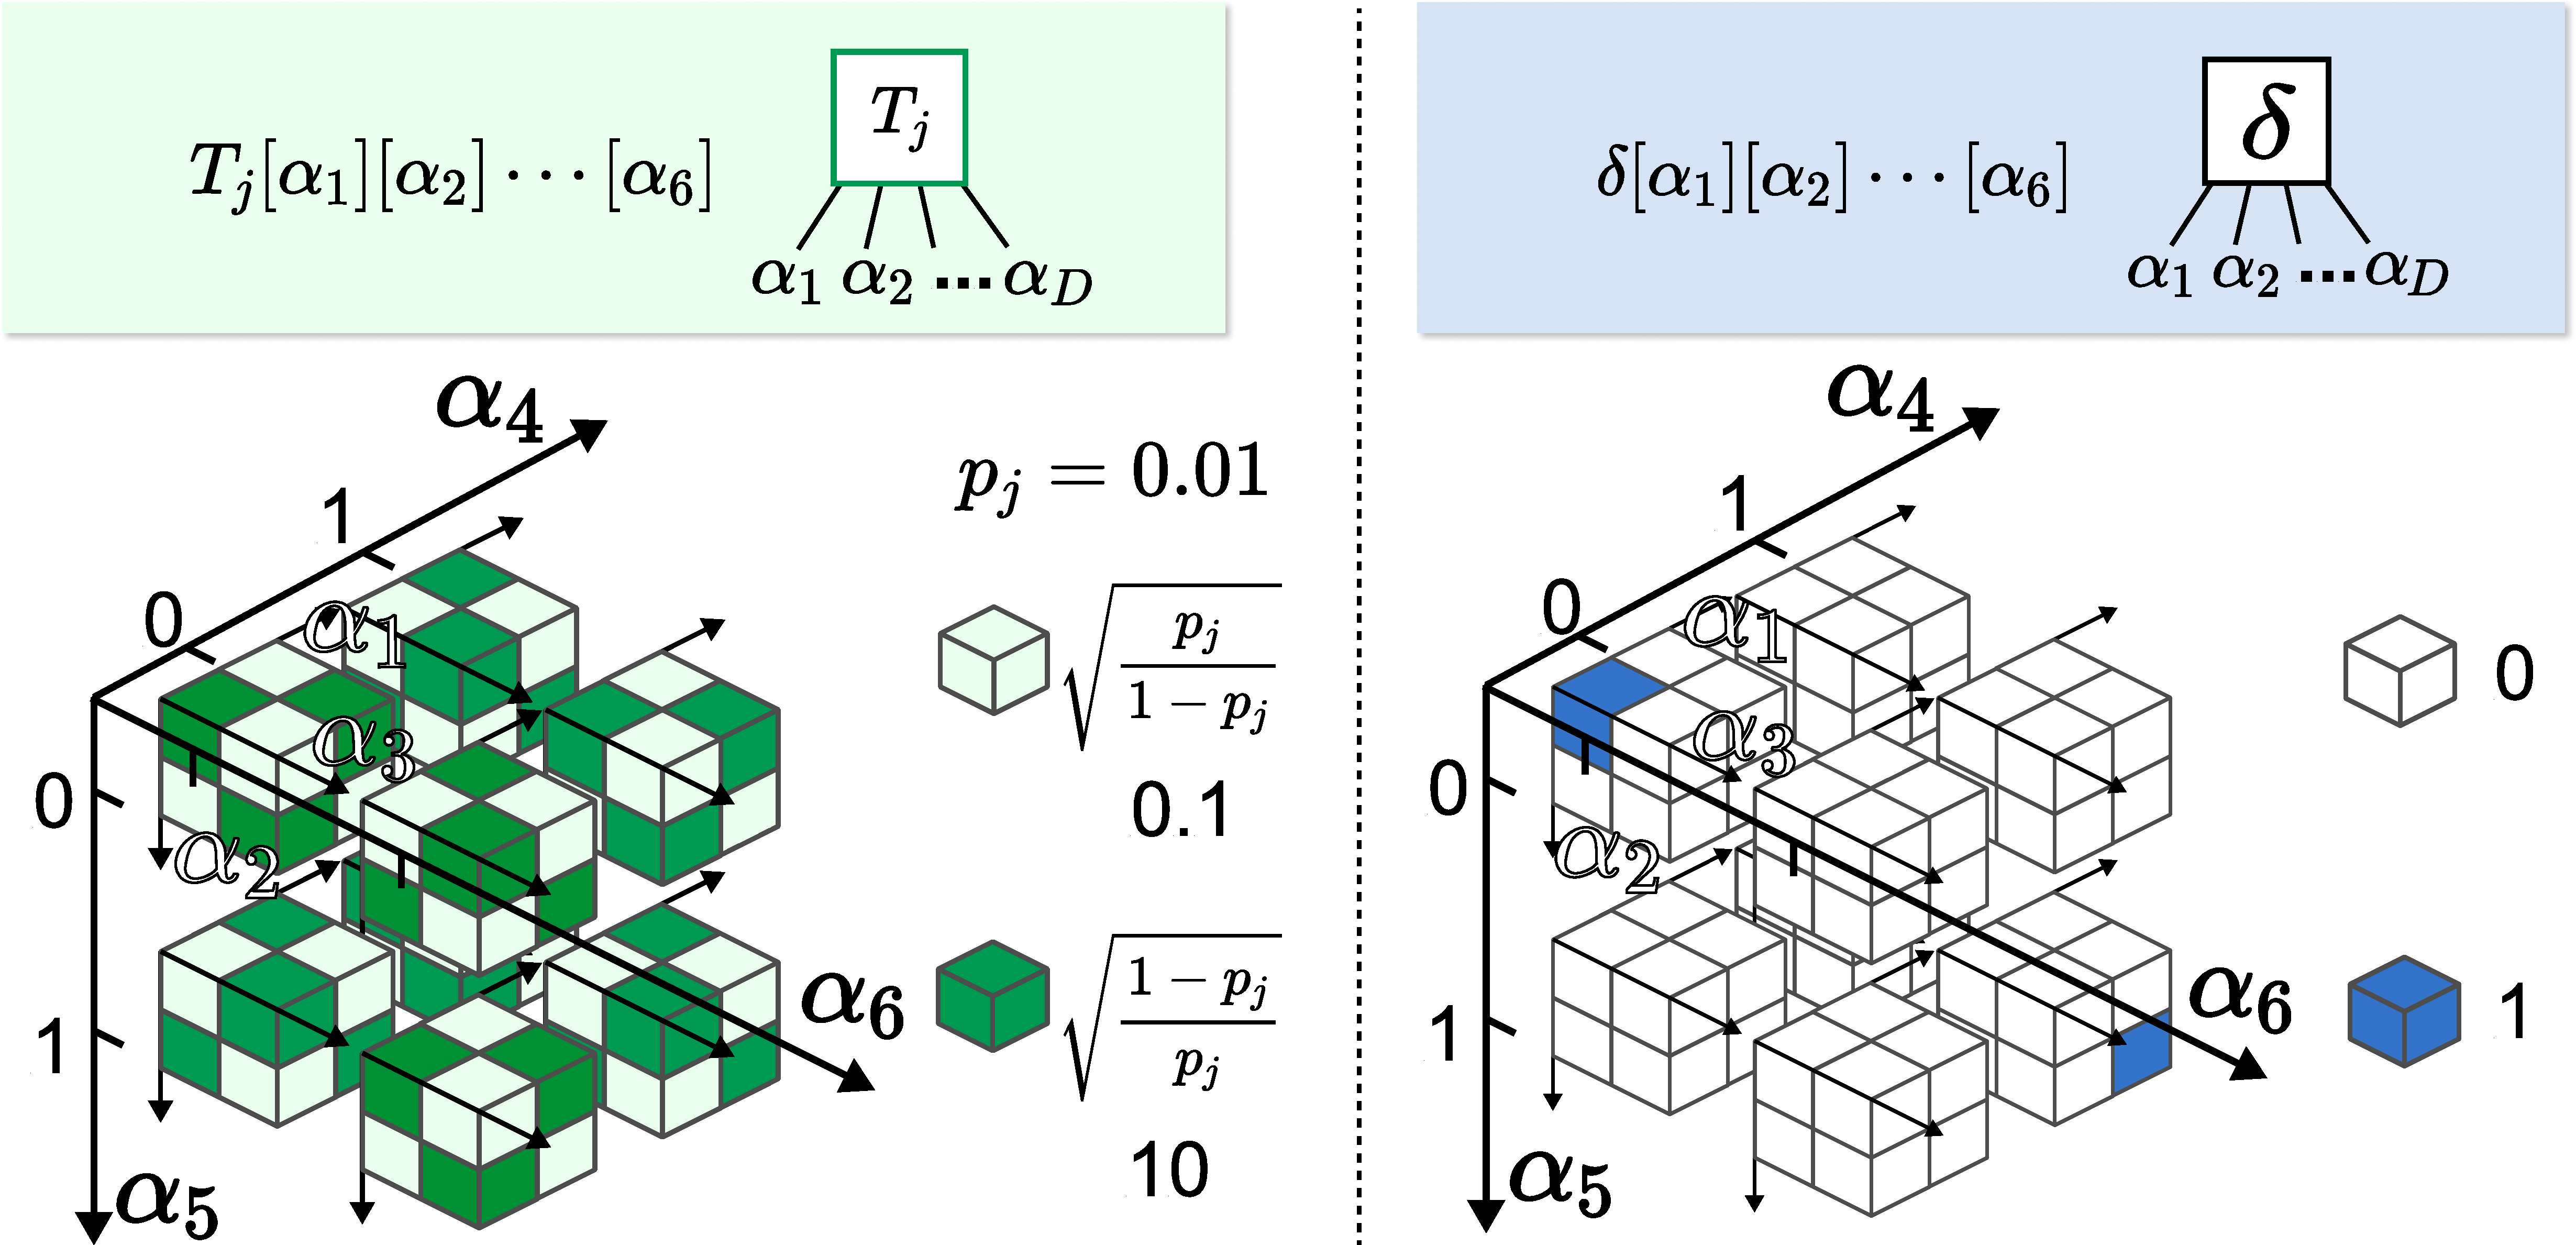
\includegraphics[width=1\columnwidth]{figures/TensorExample.pdf}}
\vspace{-0.3cm}
\caption{The numerical example of the tensors used in the tensor network decoder.} 
\label{fig:tensor_example}
\end{figure}

\subsection{Exact Tensor Decomposition via Matrix Product State}

The raw tensor network involves n-rank tensors with $2^n$ elements, leading to huge computation cost and memory bottleneck. Prior compression techniques often employ singular value decomposition to decompose the tensors into low-rank matrix product states (MPS) or tree tensor network states~\cite{pan2020contracting,ma2024approximate}. However, this coarse-grained decomposition only saves the top largest singular values of tensors and drops the other singular values, causing a significant accuracy loss.

% The tensors in the original tensor network, as shown in \autoref{fig:formulation}~(c), are high-rank tensors with $2^n$ elements, making the contraction suffer from high computation cost and memory bottleneck. Prior work on tensor network contraction using singular value decomposition to decompose the tensors into low-rank Matrix Product States (MPS) or tree tensor network states~\cite{pan2020contracting,ma2024approximate}. \hl{This decomposition only saves the top largest singular values of tensors and drops the other singular values, causing an accuracy loss. }
% \hl{why there is a great accuracy loss?}



\begin{figure}[t]
\centerline{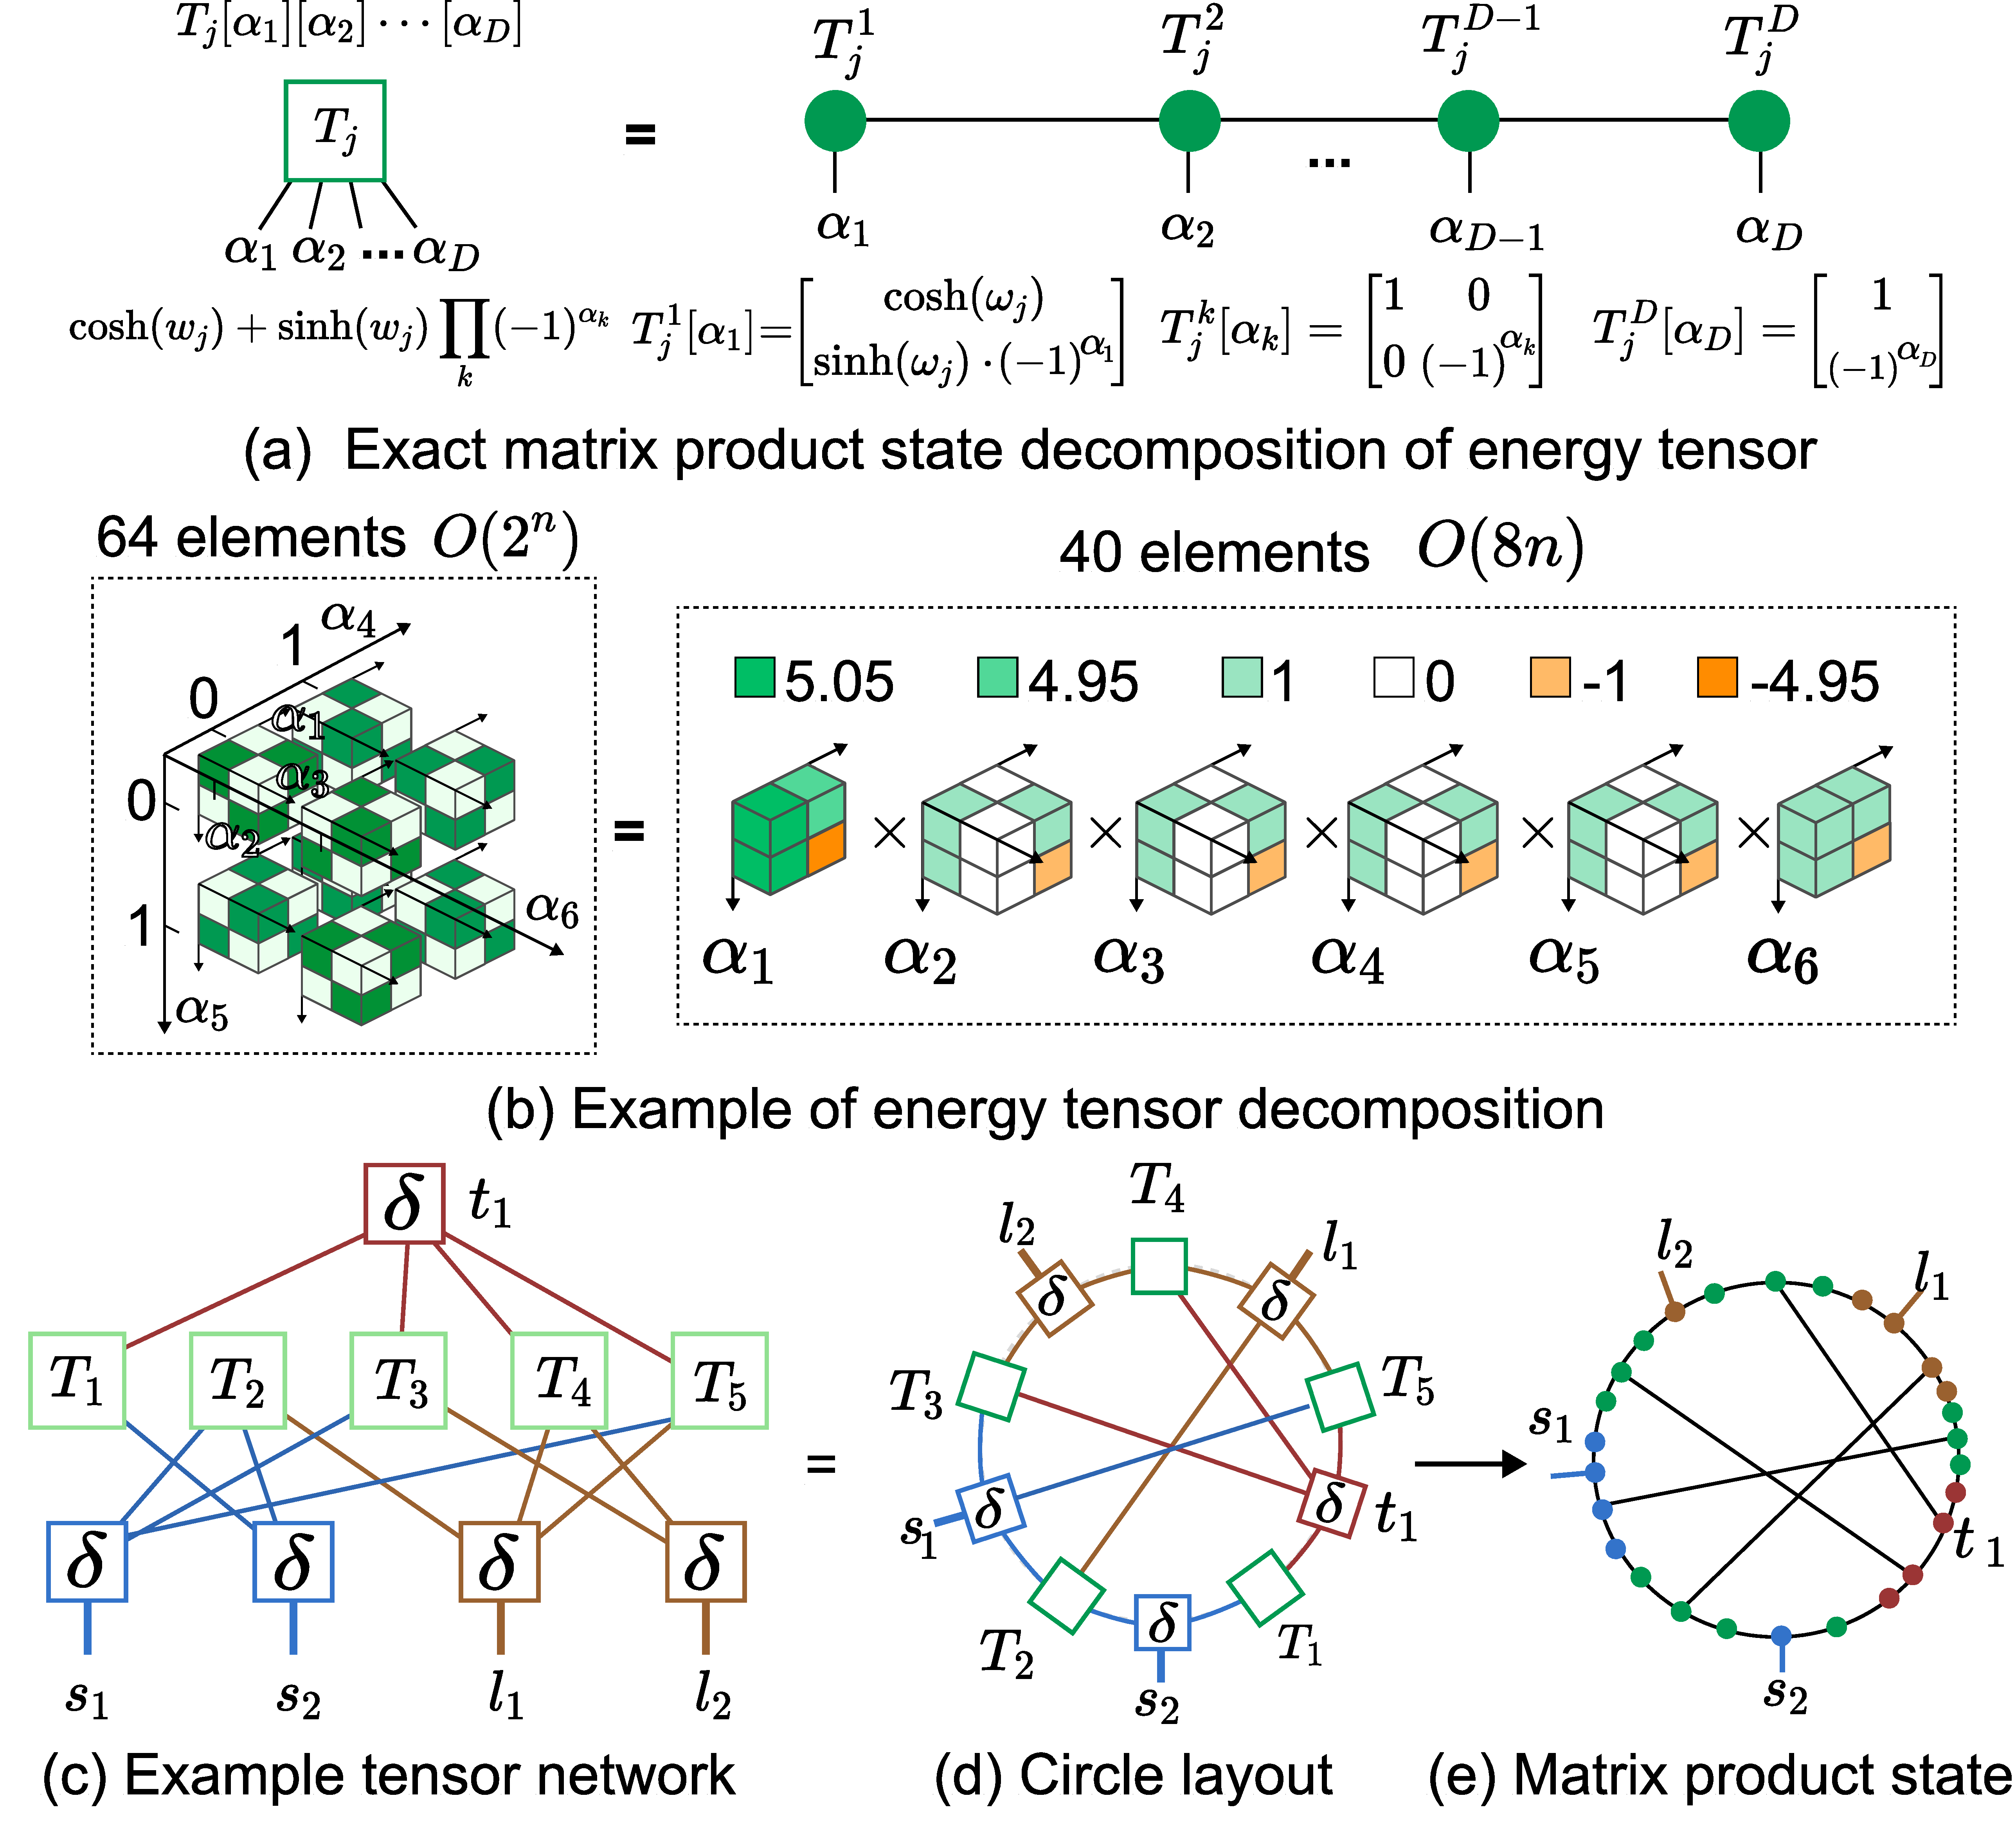
\includegraphics[width=1\columnwidth]{figures/mps.pdf}}
\vspace{-0.3cm}
\caption{Decomposing the tensor network into matrix product states.} 
\vspace{-0.2cm}
\label{fig:mps}
\end{figure}

%先讲讲我们的考虑，我们是怎么想到exact decomposition，为什么我们可以exact，再给具体数学细节
% \hl{insight, motivation, how we got this?}
Considering the binary nature of the errors and check matrices in MLD, we observe that the tensors derived from the spin glass model exhibit a highly structured nature. The pattern includes: 1) each element only has two values (\eqref{eq:tensordelta} and \eqref{eq:tensorTcases}); 2) the same values are in diagonal distribution or interleaved distribution. Identifying these features, we propose an exact decomposition scheme that can equivalently decompose the tensor into a series of smaller matrices, as
shown in \autoref{fig:mps}~(a). 
Specifically, since the results of spin multiplication only have two values, -1 or 1, the tensor can only be $e^{-\omega_j}$ and $e^{\omega_j}$, transforming the tensor $T_j$ in \eqref{eq:tensorT} to hyperbolic functions.
\begin{equation} \small
    T_j = \cosh (\omega_j) + \sinh (\omega_j) \prod_k (-1)^{\alpha_k}
\end{equation}
We can verify that this tensor $T_j$ can be represented by matrix products with the tensors $T_j^k$ in \autoref{fig:mps}~(a).
\begin{equation}\small
    T_j[\alpha_1][\alpha_2]\cdots[\alpha_D] = \prod_{k=1}^{D} T^k_j[\alpha_k]
\end{equation}
\autoref{fig:mps}~(b) gives the example of decomposing a six-rank energy tensor into six three-rank tensors, shrinking the tensor size from 64 elements to 40 elements.
For the tensor $\delta$ in \eqref{eq:tensordelta}, the elements that share the same index $\alpha_k$ have the same values. Thus, it can be exactly decomposed into low-rank tensors $\delta$.
\begin{equation}\small
    \delta[\alpha_1]\cdots[\alpha_D] = \sum_{\vec{\beta}} \delta[\alpha_1][\beta_1] \delta[\beta_1] [\alpha_2] [\beta_2]\cdots \delta[\beta_{D-1}] [\alpha_D].
\end{equation}

\autoref{fig:mps}~(c)-(e) visualizes the tensorization process of the entire tensor network, where the tensor network is derived from \autoref{fig:formulation}~(c). To better understand dimension reduction, \autoref{fig:mps}~(d) organizes it in a circular layout, maintaining the original connectivity. In this circle, we can observe that each tensor is connected with four neighboring tensors at most. By decomposing it into matrix product states, the tensors are converted into three-rank tensors or two-rank tensors, and each has at most three neighbors, as depicted in \autoref{fig:mps}~(e).

% Using the exact matrix product state decomposition, we can represent the original high-rank tensors into two-rank tensors or three-rank tensors, reducing the memory complexity from $O(2^n)$ to $O(8n)$. For instance, the tensor network in \autoref{fig:mps}~(b) contains ten tensors with four-rank at most. If we organize it in a circle layout as shown in \autoref{fig:mps}~(c), we can see that the tensors in the graph show a high-dimensional connection with four neighboring tensors at most. By decomposing it into matrix product states, the tensors are converted into three-rank tensors or two-rank tensors, and each has at most three neighbors, as depicted in \autoref{fig:mps}~(d).






\subsection{Tensor Network Compression by Offline Contraction}

Although MPS partially addresses the computational pressure, especially the memory bottleneck, there remain tremendous computations arising from the high-dimensional connections among matrices. A natural idea is to compress the connectivity offline and introduce a low-dimensional topology MPS when online decoding. Observing that the high-dimensional connection basically results from the internal edges in the circle, as shown in \autoref{fig:mps}~(d), our intuition is to eliminate these internal edges. To achieve this goal, we propose the \textit{contraction-swap-merge} method, which iteratively contracts the small tensors, swaps the tensor indices to put the internal edges in adjacent positions, and merges these edges. These three operations used in this method are defined as follows.
% \hl{three operator.}
\begin{itemize}
    \item The \textit{contract} operation is the basic operation in the tensor network, which merges two adjacent tensors into a new tensor by contracting the edge index between them, as shown in \autoref{fig:operations}~(a). The cost of \textit{contract} operations between two tensors with $d_1$ dimensions and  $d_3$ dimensions is $O(d_1d_2d_3)$, where $d_2$ is the bond dimension between them (The bond dimension is the dimension of the multiplication between two tensors). 
    
    \item The \textit{swap} operation is defined as swapping the two adjacent indices in MPS, such as the $\alpha_2$ and $\alpha_3$ indices in \autoref{fig:operations}~(b). The \textit{swap} cost differs in two cases. Swapping between pairs like $(T,T)$, $(T,\delta)$,$(\delta,\delta)$ has no cost. However, for other cases, swapping between tensors needs to use a contract operation and singular value decomposition with cost $O(d^6)$. This will introduce accuracy loss due to the singular value decomposition is an approximated Ddecomposition~\cite{ma2024approximate}. 
    
    \item The \textit{merge} operation uses two contract operations to merge the adjacent edges between two MPS into one edge with a higher dimension. The cost of the \textit{merge} operation comes from the \textit{contract} operation, as shown in \autoref{fig:operations}~(c).
\end{itemize}


% Matrix product state (MPS) solves the memory bottleneck caused by high-rank tensors but still suffers from the high contraction cost due to the high-dimensional connections between matrix product states, making the deployment on a real-time hardware decoder impractical. A natural idea is to reduce the dimension of the connection topology offline and use a low-dimensional topology matrix product state for online decoding. We further identify that the high-dimensional connection is due to the additional connection edges between each tensor, such as the edges inside the circle in \autoref{fig:mps}~(c). Our intuition is to eliminate these entanglement edges and obtain a tensor network with only tensors on the circle, which is exactly a 1D-chain matrix product state that can be efficiently stored and contracted. To execute this strategy, we designed a \textit{swap-merge-contraction} method. 


\begin{figure}[t]
\centerline{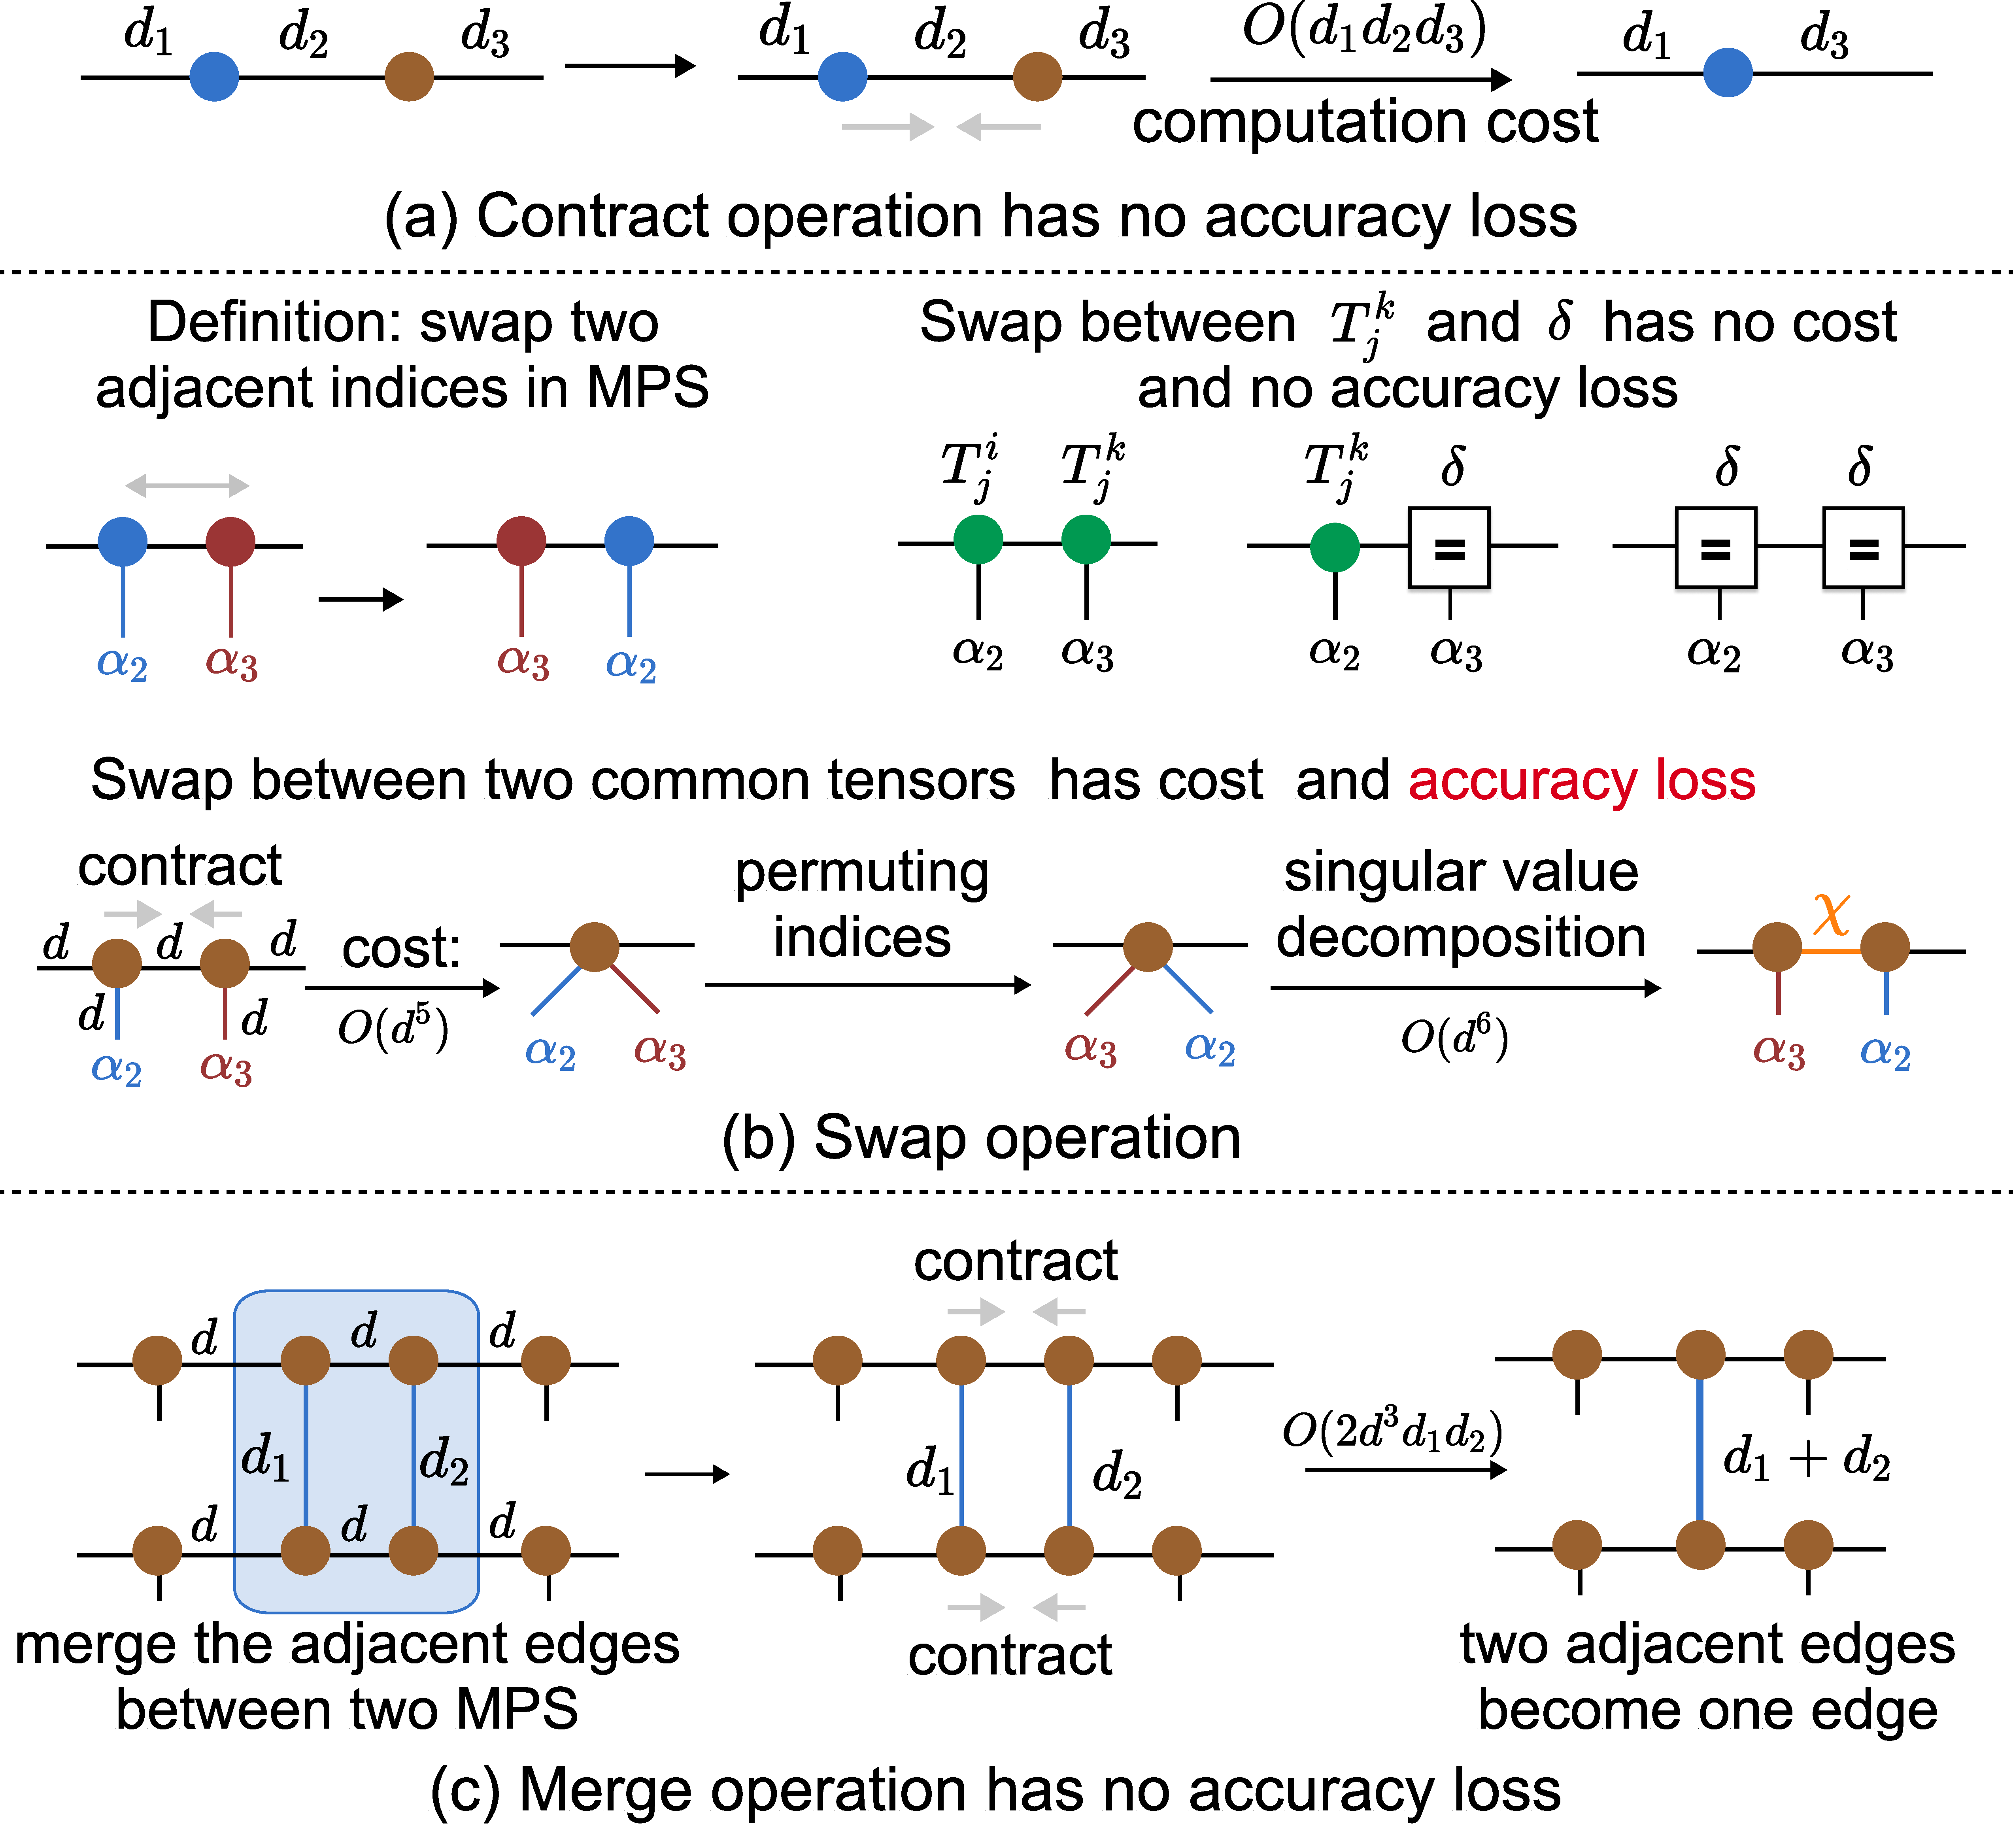
\includegraphics[width=1\columnwidth]{figures/operations.pdf}}
\vspace{-0.4cm}
\caption{Operations definition and cost in offline contraction.} 
\vspace{-0.4cm}
\label{fig:operations}
\end{figure}

\begin{algorithm}[t]
\small
\caption{Contraction-swap-merge Algorithm} \label{algo:contraction}
\KwIn{Tensor network with tensors \( A^{(1)}, \dots, A^{(n)} \), connectivity Tanner graph \( G(V, E) \), set of tensors with outer logical and syndrome indices \( P \subseteq V \)}
\KwOut{1D-chain MPS containing tensors in \(P \)}
Exactly decompose every tensor to MPS\label{line:decompose}\;
\While{\( \exists v \notin P \)}{\label{line:while}
    Find edge \( (i, j) \gets \arg\min_{(\mu, \nu) \in E, \{ \mu, \nu \} \not\subseteq P}  \) \( [ \sum_{b \in \partial \mu} \log(D_{b,\mu})  + \sum_{b \in \partial \nu} \log(D_{b,\nu}) - 2 \log(D_{\mu,\nu})] \) \label{line:argmin}\;
    Move tensor at edge \( (i, j) \) in \( A^{(i)} \) to MPS tail \label{line:move_tail}\;
    Move tensor at edge \( (i, j) \) in \( A^{(j)} \) to MPS head \label{line:move_head}\;
    \textit{Contract} edge \( (i, j) \) to combine MPS \( A^{(i)} \) and \( A^{(j)} \) into a new MPS\label{line:merge}\;
    Update \( E \gets E \setminus \{(i, j)\} \) \label{line:remove_edge}\;
    \For{\( k \in \partial j \)}{\label{line:for}
        Remove \( (j, k) \) from \( E \) \label{line:remove_jk}\;
        \eIf{\( k \in \partial i \)}{\label{line:if}
            \textit{Swap} to place duplicate edges \( (i, k) \) adjacent in \( A^{(i)} \) \label{line:swap}\;
            \textit{Merge} adjacent tensors, combining edges to increase \( D_{k,i} \) \label{line:merge_tensors}\;
        }{
            Add \( (i, k) \) to \( E \) \label{line:add_edge}\;
        }
    }
    \eIf{\( j \in P \)}{
        Add \( i \) to \( P \) \label{line:add_p}\;
    }{
        Update \( V \gets V \setminus \{j\} \) \label{line:remove_node}\;
    }
}
\Return the 1D-chain MPS\label{line:return}\;
\end{algorithm}


% trade-off, algorithm

As we can see, the \textit{swap} operation is an approximation operation with some accuracy loss. Thus, we propose a greedy algorithm to reduce the use of the \textit{swap} operations, as shown in Algorithm~\ref{algo:contraction}. We use a graph \( G(V, E) \) to denote this tensor network, the node \( V \) representing the tensors and edges \( E \) representing the connected indices between tensors $A^{(i)},A^{(j)}$ with a bond dimensions \( D_{i,j} \). The initial bond dimension is 2. Tensors with outer logical and syndrome indices in set \( P \) are preserved, forming a 1D matrix product state chain as output. 
% The edges are contracted iteratively based on minimal cost, preserving outer indices. Bond dimensions exceeding \( \hat{D} \) are truncated via SVD. The process stops when a 1D chain of tensors with outer indices remains, returned as \( Z \).
Specifically, we first decompose the tensors into MPS representation using the exact decomposition (Line \ref{line:decompose}). Then the algorithm loops until all nodes are in the preserved set  \( P \) (Line \ref{line:while}), stopping at a 1D chain. It selects the edge \( (i, j) \) with minimal contraction cost (Line \ref{line:argmin}), moves tensors in \( A^{(i)} \) to the tail (Line \ref{line:move_tail}) and in \( A^{(j)} \) to the head (Line \ref{line:move_head}), then merges them by contracting edge \( (i, j) \) (Line \ref{line:merge}). The edge is removed from \( E \) (Line \ref{line:remove_edge}). For each neighbor \( k \) of \( j \) (Line \ref{line:for}), edge \( (j, k) \) is removed (Line \ref{line:remove_jk}). If \( k \) connects to \( i \) (Line \ref{line:if}), duplicate edges \( (i, k) \) are swapped to be adjacent (Line \ref{line:swap}) and merged, increasing \( D_{k,i} \) (Line \ref{line:merge_tensors}). If \( k \) is not connected to \( i \), edge \( (i, k) \) is added to \( E \) (Line \ref{line:add_edge}). If \( j \in P \), \( i \) is added to \( P \) (Line \ref{line:add_p}); otherwise, \( j \) is removed from \( V \) (Line \ref{line:remove_node}). The final 1D MPS chain is returned (Line \ref{line:return}).

\begin{figure}[t]
\centerline{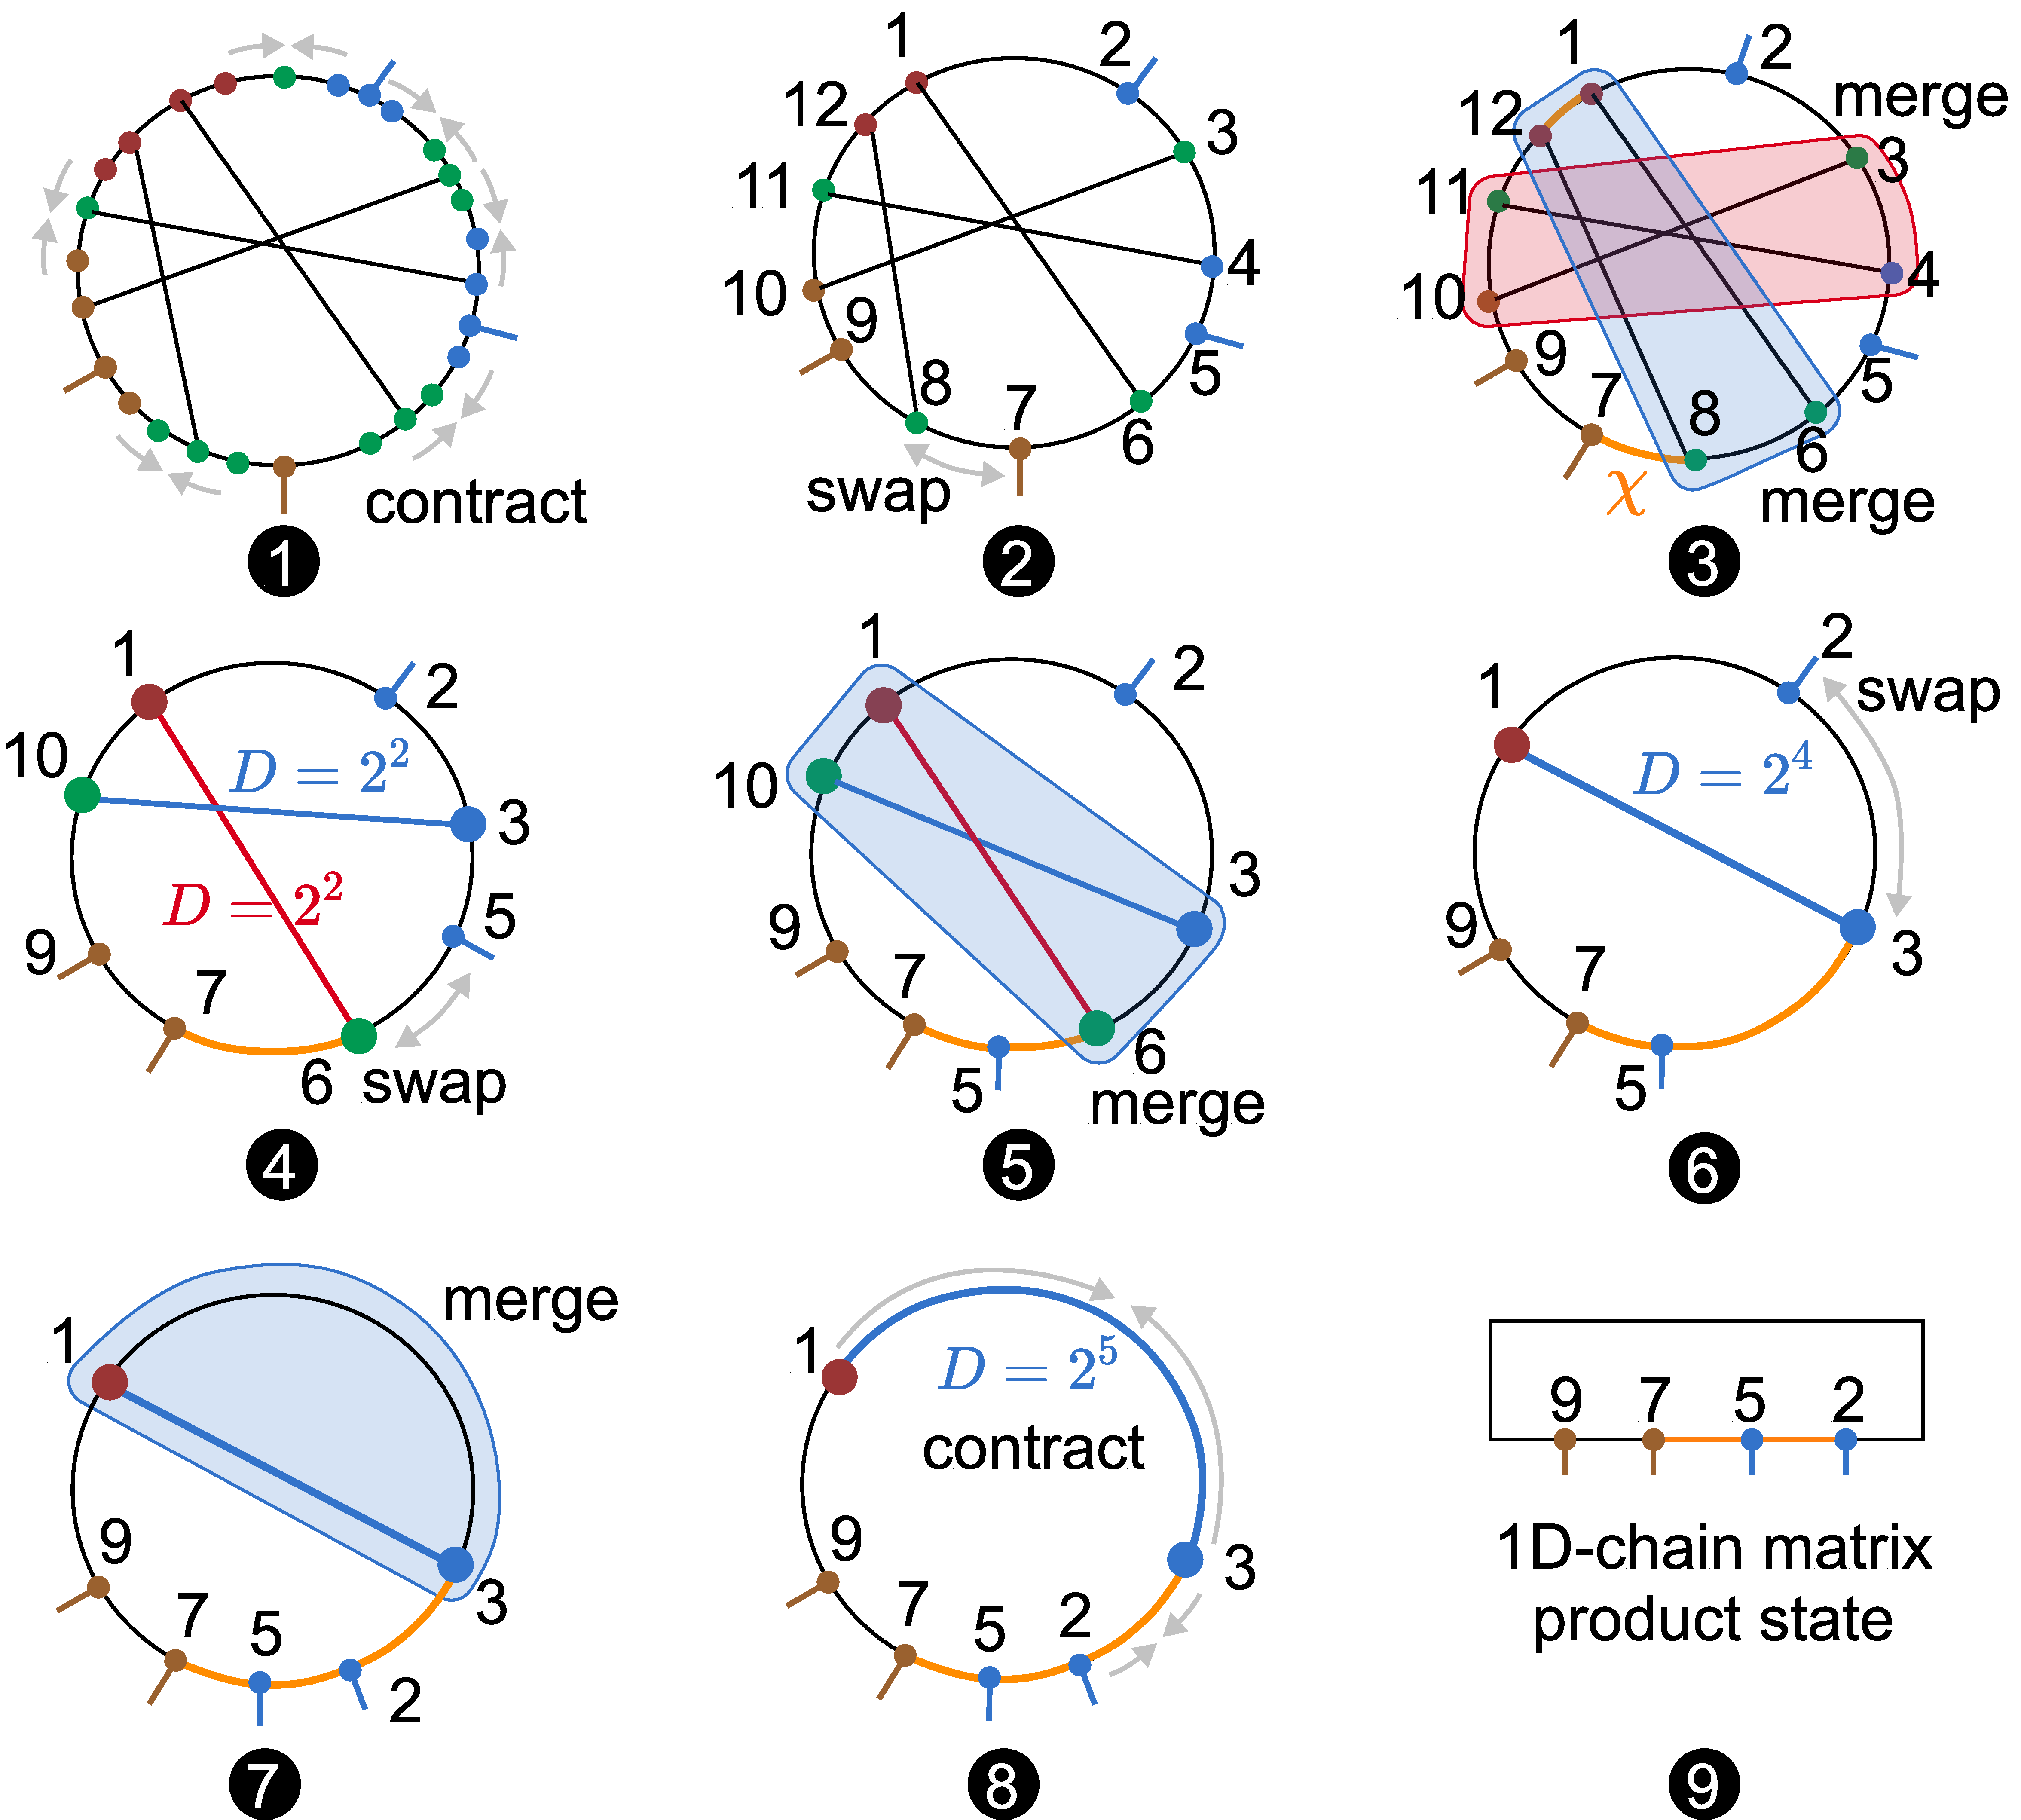
\includegraphics[width=0.9\columnwidth]{figures/circlecontraction9.pdf}}
\vspace{-0.2cm}
\caption{Offline contraction to get the approximated matrix product state for free energies under different syndromes.} 
% \vspace{-0.4cm}
\label{fig:contraction}
\end{figure}



\autoref{fig:contraction} gives an example of the \textit{swap-merge-contraction} approach. We start by \textit{contract} the edges in the MPS representation with the lowest contraction costs as shown in step~\ding{182}. Then we \textit{swap} the two MPS in edge (8,7) as step~\ding{183} to make the two pairs of edges (12,8) and (1,6) in adjacent positions as step~\ding{184}. We \textit{merge} the two pairs of edges \{(12,8) and (1,6), (11,4) and (10,3) \} into two new edges with the bond dimension $D=2^2$ as shown in step~\ding{185}. The steps \ding{185}-\ding{188} also repeat this \textit{swap} and \textit{merge} process until no edges are inside the circle. Then, we \textit{contract} the matrices (1,3) on the circle as in step~\ding{189}, except for the tensors \{9,7,5,2\} with outer logical and syndrome indices, to obtain a 1D-chain MPS with only logical and syndrome indices, as shown in step~\ding{190}.


\section{\papername Decoding Flow and Architecture}

When using the 1D-chain matrix product state for decoding, directly enumerating all logical spins will incur exponential complexity with the number of logical qubits. Thus, we develop a partial tracing strategy to compute the conditional marginal probability of each logical spin in parallel. This strategy takes only $O(M\chi^2+\log K \cdot K^2\chi^4)$ with the number of syndrome checks $M$, the number of logical qubits $K$, and the virtual bond $\chi$  (the dimension of the matrix) of matrix product states, meanwhile maintaining the accuracy of decoding. Based on this polynomial-time decoding flow, we design a dedicated hardware architecture and implement it on the GPU device. We leverage the tensor core for matrix product and the CUDA core for calculating the marginal logical probabilities.

\subsection{Online Decoding via Conditional Marginal Probability}

The 1D-chain MPS contains the free energy under all syndromes and logical spin configurations. The decoding goal is to find the logical spin configuration with minimal free energy when given the syndrome spins. Directly enumerating all logical spin configurations needs $O(2^K(M+K)\chi^3)$, where $K$ is the number of logical qubits, $M$ is the number of syndrome qubits, and $\chi$ is the maximum virtual bond of the 1D-chain MPS.

To overcome the enumeration, we propose to calculate the marginal probability of each logical spin. The marginal probability is computed as 
\begin{equation}\small
    P(l_i=1|\vec{s}) = 
    \frac{{\text{contract}}(\mathcal{T}(l_i=1,\vec{s}))}{\text{contract}(\mathcal{T}(\vec{s}))}. 
    \label{}
\end{equation}
This means we only need to contract the 1D-chain MPS twice under the values of $g_i$ to get the marginal probability. However, using the marginal probability may not determine the value of logical spin $g_i$. For example, when the marginal probability is around 0.5, the value of logical spin can be 1 or -1 with the same probability. To find the most likely logical spin values, we further calculate their conditional probability under the determined spin values. 




\begin{figure}[t]
\centerline{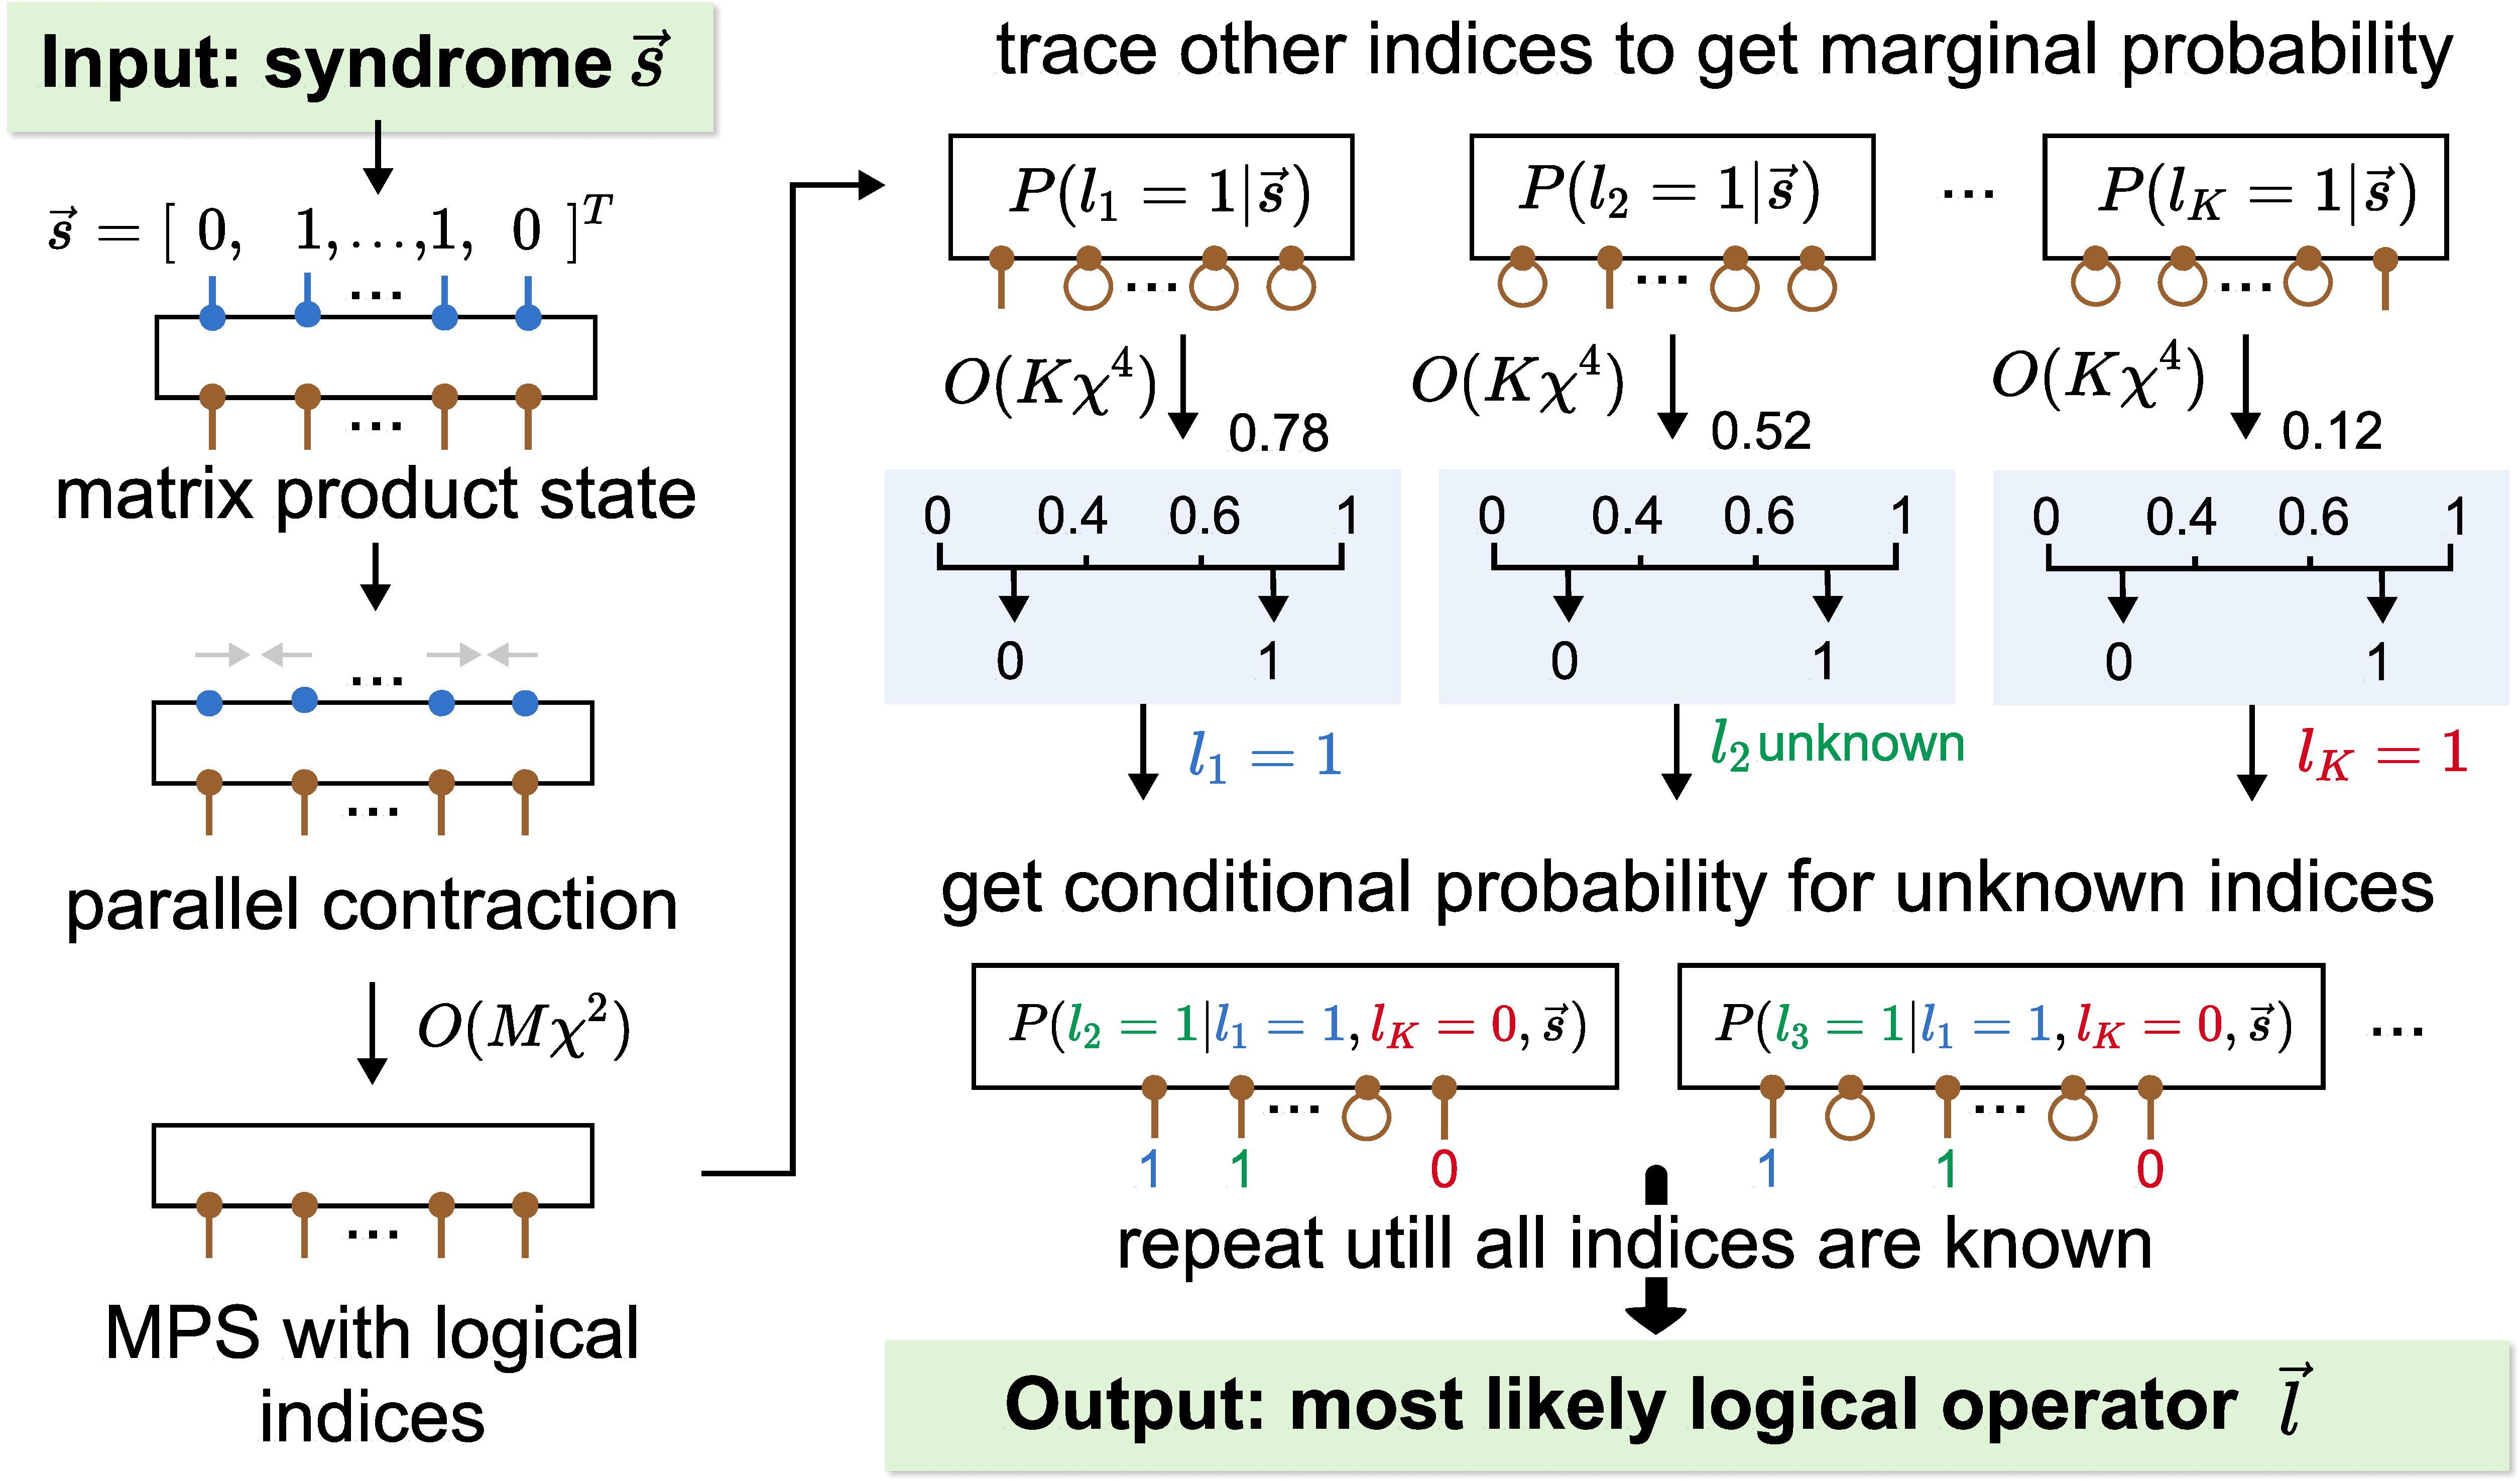
\includegraphics[width=0.98\columnwidth]{figures/logicaldecoding.pdf}}
\vspace{-0.2cm}
\caption{Online decoding via marginal probability calculation.} 
\vspace{-0.4cm}
\label{fig:decoding}
\end{figure}

\textbf{Online decoding flow and complexity analysis}.
\autoref{fig:decoding} illustrates the proposed online decoding flow. The decoder takes the measured syndrome vector $\vec{s}$ as input, representing the outcomes of stabilizer measurements. The MPS e
ncodes the free-energy landscape over all syndrome–logical spin configurations. Given $\vec{s}$, we contract the MPS to obtain one involving only logical spin indices, with a cost of $O(M\chi^2)$, where $M$ is the syndrome length and $\chi$ the maximum bond dimension. To determine the optimal logical spin configuration $\vec{l}$, the marginal probability of each logical spin $l_i$ is computed in parallel by tracing over other indices, requiring $O(K\chi^4)$ computation, where $K$ is the number of logical spins. Spins with probabilities close to 0 or 1 are fixed directly, while ambiguous ones (around 0.5) are refined through local conditional contractions, iterated $O(\log K)$ times. Finally, the recovered logical operator $\vec{l}$ is used to correct the physical state via the~\eqref{eq:recovererror}. This hierarchical contraction strategy reduces complexity from exhaustive enumeration to $O(M\chi^2+\log K\cdot K^2\chi^4)$ sequentially and $O(M\chi^2+\log K\cdot K\chi^4)$ in parallel, enabling scalable decoding.


\subsection{Hardware Architecture of Online Decoding}

\begin{figure}[t]
\centerline{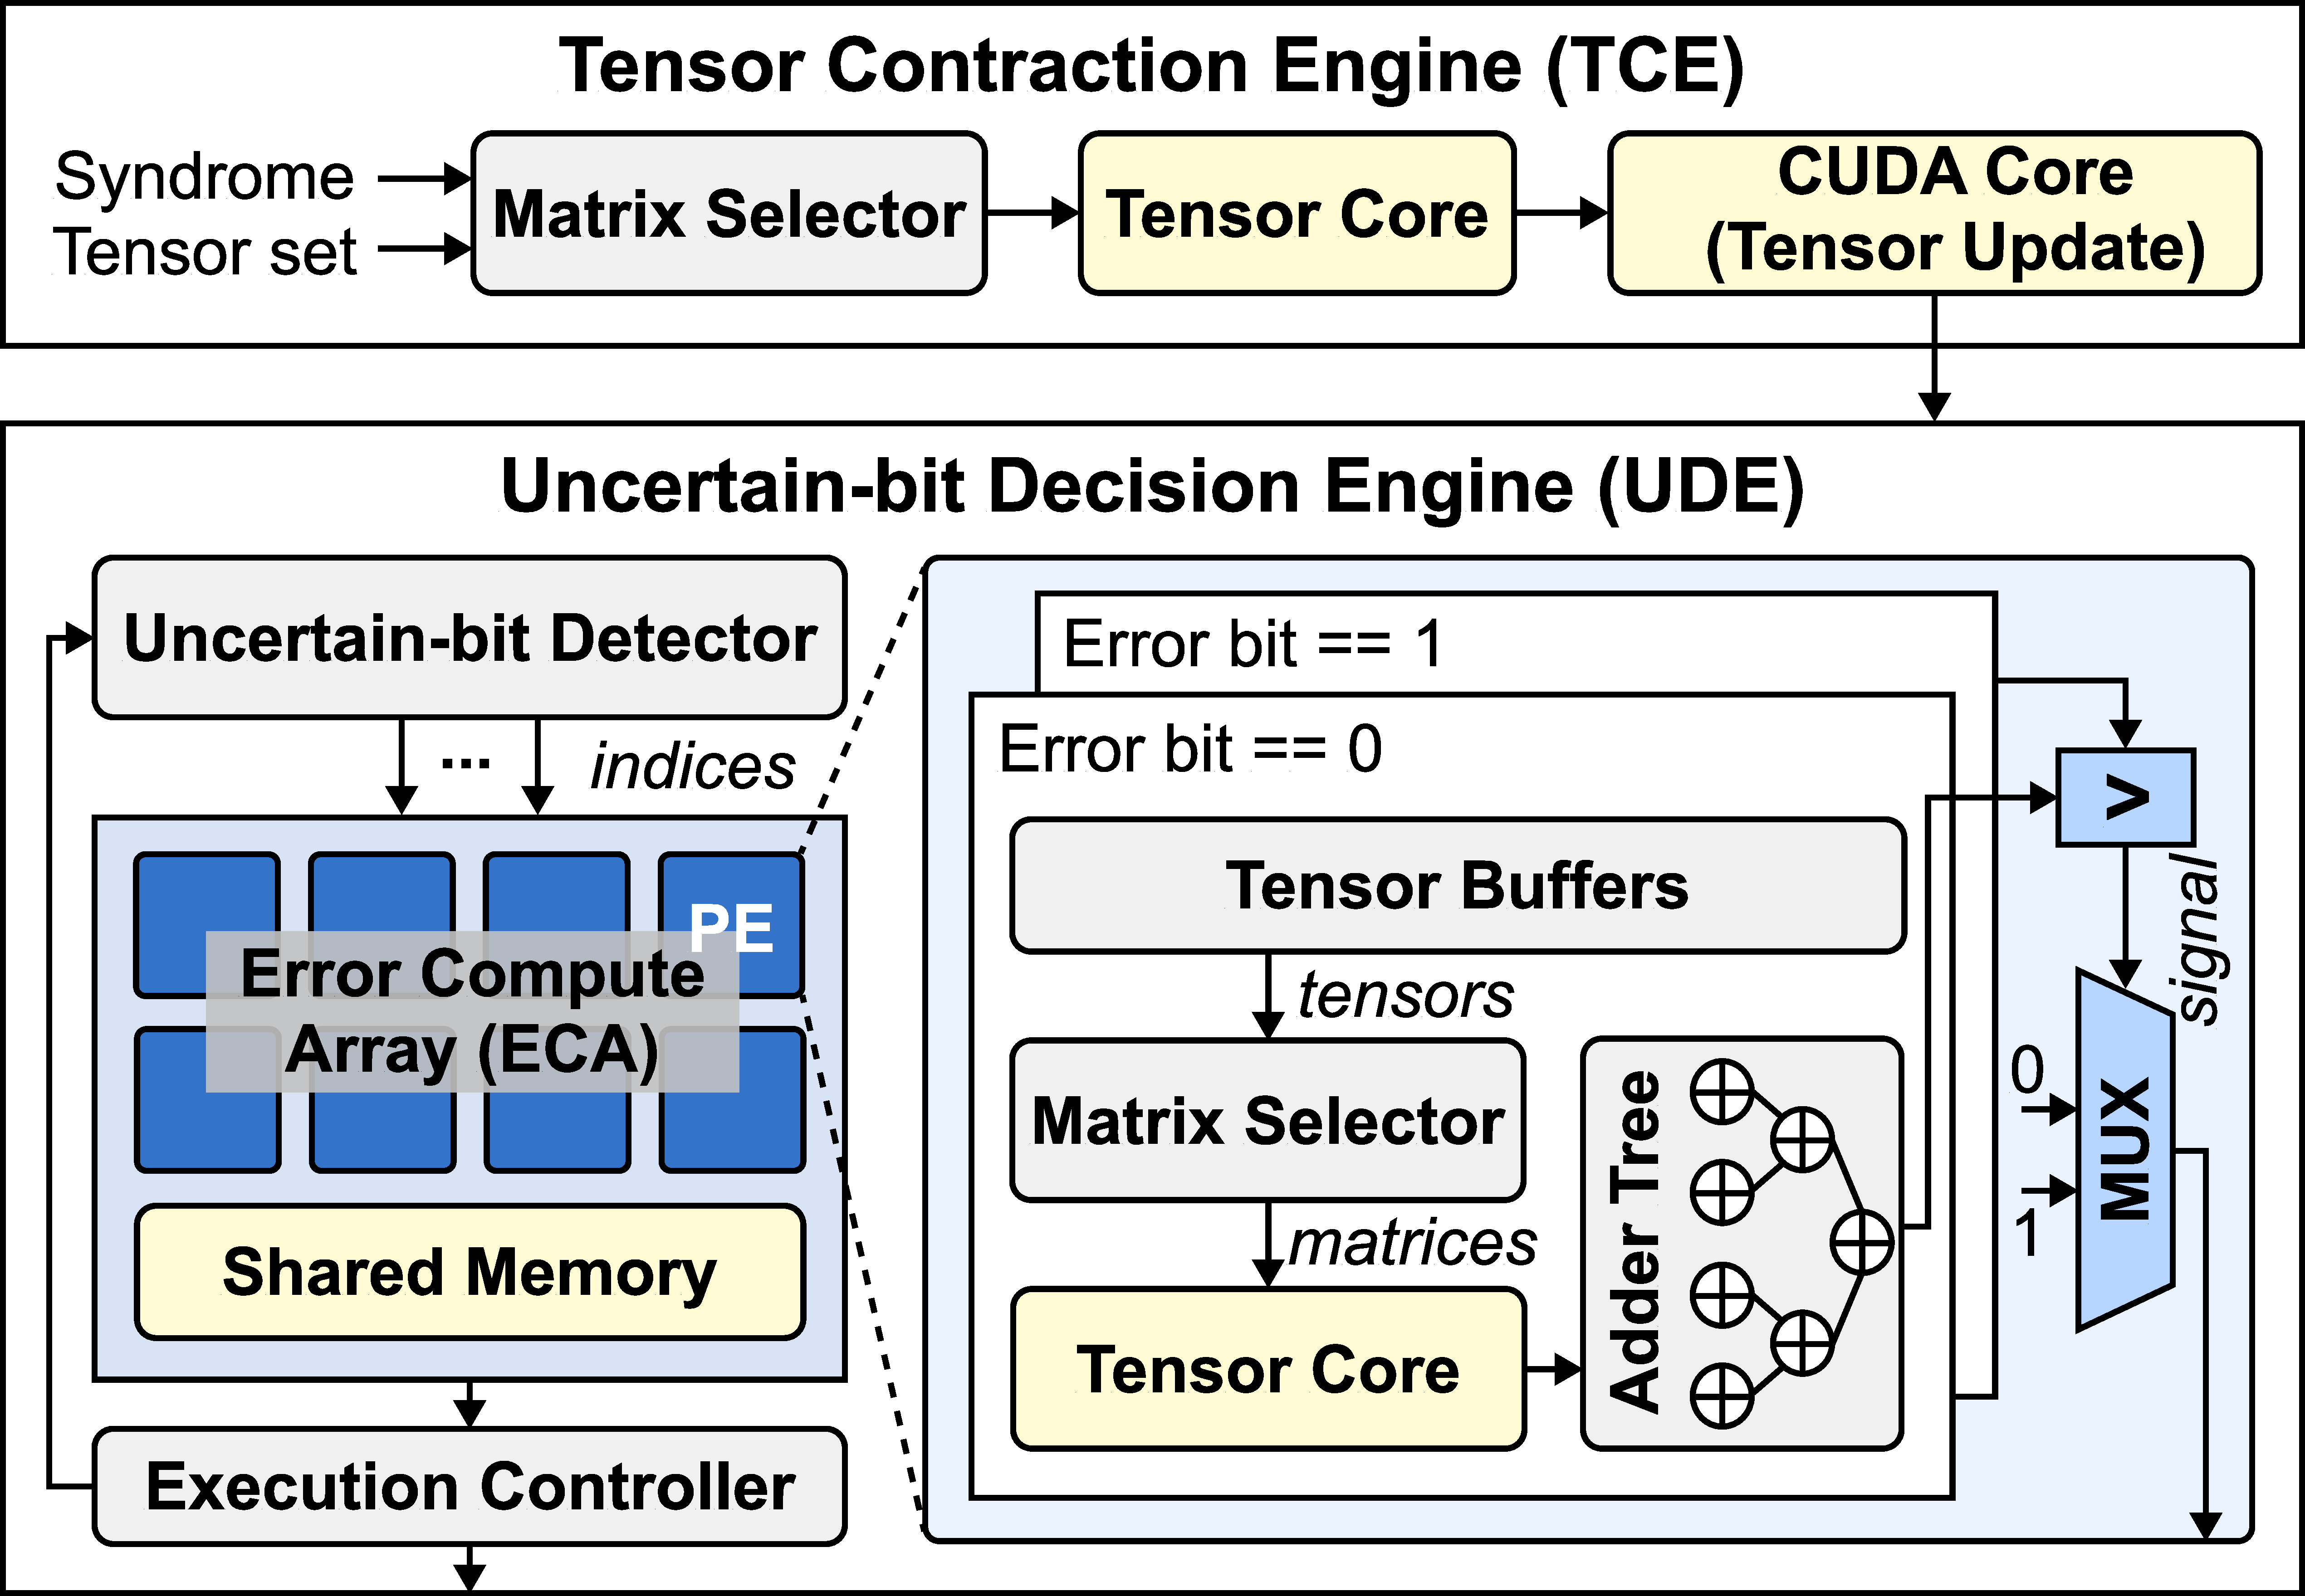
\includegraphics[width=0.95\columnwidth]{figures/gpu_hardware.pdf}}
\vspace{-0.2cm}
\caption{Hardware architecure support for \papername online decoding.} 
\vspace{-0.2cm}
\label{fig:gpu_hardware}
\end{figure}

\autoref{fig:gpu_hardware} presents the \papername hardware architecture designed to support the online decoding computational flow. The architecture consists of two major components: (1) a tensor contraction engine (TCE) and (2) an uncertain-bit decision engine (UDE). The TCE takes the syndrome and the tensor set as inputs. It leverages tensor cores to perform matrix multiplications in parallel and stores intermediate contraction results in shared memory to minimize global memory traffic during iterative tensor updates. A tensor update unit implemented using CUDA cores constructs the 1D-chain MPS with only $K$ tensors and writes them back to the on-chip tensor buffer. Once the MPS chain is generated, it is streamed to the UDE for determining the most probable logical spin configuration.

Within the UDE, an uncertain-bit detector identifies unknown logical indices whose marginal probabilities fall into the uncertainty and dispatches them to the error compute array (ECA). The ECA consists of multiple processing elements (PEs), each dedicated to resolving one uncertain bit. In each PE, the likelihoods for the spin value equal to 0 and 1 are computed in parallel. Specifically, a matrix selector first retrieves the relevant tensors from the on-chip tensor buffers (in shared memory) and feeds the selected matrices to tensor cores. The resulting matrix is then sent to an adder tree implemented by CUDA core–based parallel reductions, which accumulates its diagonal elements to compute the likelihood. Then, we compare the two likelihoods to determine the final value. All uncertain bits are processed in parallel across the PEs to maximize concurrency. Finally, an execution controller monitors whether unresolved bits remain in the logical operator $\vec{l}$. If so, it triggers another round of refinement; otherwise, the decoding process terminates.

% Looking forward, several stages of the pipeline can benefit from FPGA-based design. For example, the tensor update path in the TCE can be mapped to a fully pipelined contraction unit with a scratchpad hierarchy, removing the general-purpose overheads of tensor cores. Likewise, the uncertain-bit detector of UDE matches FPGA spatial parallelism: each PE can be implemented as a hardwired datapath with fixed matrix selection and reduction logic, enabling deterministic per-bit processing. In addition, a lightweight FPGA control engine can orchestrate refinement rounds without GPU scheduling overhead. With these customized modules, the end-to-end latency can be reduced substantially. For instance, a GPU-bound latency on the order of $10^3 \mu s$ can be decreased to sub-$10^1 \mu s$, yielding both higher throughput and better energy efficiency than a pure GPU design.
% \section{\papername Tensorization and Compression} \label{sec:formulation}

\begin{figure*}[t]
\centerline{
\includegraphics[width=1\textwidth]{figures/formulation.pdf}}
\vspace{-0.2cm}
\caption{Formulating the (a) maximum likelihood decoding as (b) minimizing the free energy of the spin glass model, and using (c) the tensor network to calculate the free energy.} 
\vspace{-0.4cm}
\label{fig:formulation}
\end{figure*}

To balance the decoding accuracy and computational complexity, we first convert the constrained calculation into an unconstrained summation format. Then, the computation for this summation is tensorized using the spin glass model, where 
the errors and syndromes are converted into spins. After this, the logical probabilities are calculated by the free energies of the spin glass system, which can be efficiently computed by the tensor network.
Although the tensorization exposes the opportunity to parallel the MLD computation, the overall memory footprint and computational workload (FLOPs) still grow exponentially with the qLDPC code size. Identifying that the tensors from the spin glass model can be expressed by a product of constant-dimensional matrices, we propose an exact tensor decomposition that shrinks the original $O(2^n)$ tensor to a matrix product state (MPS) with a linear complexity of $O(8n)$, from 
3.9GB to 8.7KB for 254-size trivariate bicycle codes. To further reduce the computational workload, we flatten the high-dimensional connection in MPS into a 1D chain. We achieve this by swapping the tensor indices and merging adjacent matrices to eliminate high-dimensional connections without loss of logical probability information. Finally, we successfully compress the computation requirement from 6.1 TFLOPS to 48 KFLOPS, with little accuracy loss.



\subsection{Tensorizing MLD with Spin Glass Model}

Calculating the logical error probability with \eqref{eq:logicalprobcons} is non-trivial, as we need to determine the total probability by scanning all physical errors that satisfy two constraints: 1) belong to the same logical error.  2) produce the observed syndrome;
Since checking these two constraints will consume computing resources, we tend to convert the formula into an unconstrained summation format. Clearly, as shown in \autoref{fig:formulation}~(a), we decompose the logical error space $\vec{e}_Z$ into stabilizer subspaces $H_Z^T$ that are shifted by destabilizers $H_{\text{des}}^T$ and logical operators $L_Z^T$,
\begin{equation}\small
    \vec{e}_Z= H_Z^T \vec{z} \oplus H_{des}^T\vec{s}\oplus L_Z^T\vec{l},\forall \vec{z}\in\{0,1\}^M
\end{equation}
Combining this equation with the logical probability $P(\vec{l}|\vec{s})$ in \eqref{eq:logicalprobcons} gives an unconstrained summation over all possible stabilizers $\vec{z}$ as
\begin{equation}\label{eq:logicalstabsummation}
    P(\vec{l}|\vec{s}) =  \textstyle  \sum_{\vec{z} \in \{0,1\}^M} P(H_{\text{des}}^T \vec{s} \oplus H_Z^T \vec{z} \oplus L_Z^T \vec{l})\;.
\end{equation}
The mathematical derivation is summarized in \hyperref[subsec:proofA]{Appendix A}.

However, this summation still has exponential complexity.
To further simplify this, we recast the decoding problem within the framework of the spin glass model, which has broad application in discrete optimization problems~\cite{wiki_spin_glass}. A representative application is that this model is widely used in statistical mechanics to study systems with disorder and frustrated interactions, matching the properties of our formulation. Concretely, the error in decoding problem has two discrete states, 0 or 1, which resemble the two states in the spin glass model, the up(+1) and down(-1) spin rotations. This inspires us to represent stabilizer bits $\vec{z}$, syndrome $\vec{s}$, and logical bits $\vec{l}$ in ~\eqref{eq:logicalstabsummation} as stabilizer spins $\vec{t}$, syndrome spins $\vec{y}$ and logical spins $\vec{g}$ via the bits-to-spin mapping,
\begin{equation}
    (-1)^{z_k} = t_k, ~~(-1)^{s_k} = y_k, ~~(-1)^{l_k} = g_k\;.
\end{equation}
As shown in \autoref{fig:formulation}~(b), mapping bits to spins transforms the probability into the energy of a spin glass determined by the Hamiltonian $H$,
\begin{equation}\small
    H = -\sum_{j=1}^{n} \omega_j\prod_{\{k|H_z(k,j)\neq0\}} t_k  \prod_{\{k|H_{\text{des}}(k,j)\neq0\}} y_k  \prod_{\{k|L_z(k,j)\neq0\}} g_k \;.
\end{equation}
 The logical error probability under the spin glass system is
\begin{equation}\small\label{eq:logicalprobfreeenergy}
    P(\vec{l}|\vec{s})=  \textstyle \sum_{\vec{t}\in\{-1,1\}^{M}} e^{-H}
\end{equation}
The mathematical derivation is summarized in \hyperref[subsec:proofB]{Appendix B}. 

% This equation is related to the free energy $F$ of the spin glass model in statistical mechanics by $F = -\ln P(\vec{l}|\vec{s}) $~\cite{chubb2021statistical}. 
Finally, it has been demonstrated that the spin glass model can be efficiently calculated via a tensor network~\cite{cao2025exact}, exposing the opportunity to tensorize \eqref{eq:logicalprobfreeenergy}. By mapping the energy terms and spin variables in \autoref{fig:formulation}~(b) to the energy tensor $T_j$ and Kronecker Tensor $\delta$, we convert the summation operation in \eqref{eq:logicalprobfreeenergy} into the contraction of the tensor network $\mathcal{T}$ in \autoref{fig:formulation}~(c). As a result, the logical error probability $P(\vec{l}|\vec{s})$ is reformulated as the contraction of the tensor network $\mathcal{T}$. Here is the formal lemma, where the proof can be found in \hyperref[subsec:proofC]{Appendix C}.
\begin{lemma}\label{theorem:decodingTensor}
    The probability of logical error $\vec{l}$ with given syndrome $\vec{s}$, noted as $P(\vec{l}|\vec{s})$, can be calculated via tensor network $\mathcal{T}$ contraction as
    \begin{equation}\small
    P(\vec{l}|\vec{s}) = 
    \frac{{\text{contract}}(\mathcal{T}(\vec{l},\vec{s}))}{\text{contract}(\mathcal{T}(\vec{s}))}. 
    \end{equation}
\end{lemma}

% Since the spin glass model can be efficiently calculated via a tensor network~\cite{cao2025exact}, we thus try to convert \eqref{eq:logicalprobfreeenergy} into tensor computations.
% Through mapping the energy terms and spin variables in \autoref{fig:formulation}~(b) to the energy tensor $T_j$ and Kronecker Tensor $\delta$, we convert the summation operation in \eqref{eq:logicalprobfreeenergy} into the contraction of the tensor network $\mathcal{T}$ in \autoref{fig:formulation}~(c).
% % Typically, the free energy of the spin glass model can be efficiently computed with contraction on the tensor network $\mathcal{T}$ in \autoref{fig:formulation}~(c)~\cite{cao2025exact,chubb2021statistical}.
% Finally, the logical error probability $P(\vec{l}|\vec{s})$ is calculated with the contraction of the tensor network $\mathcal{T}$, as formally stated in the following lemma.


This tensor network $\mathcal{T}$ contains energy tensor $T_j$ and Kronecker tensor $\delta_i$, which are defined as
\begin{equation} \label{eq:tensorT}\small
    T_j[\alpha_1][\alpha_2]\cdots= \exp \left(\omega_j \prod_{k} (-1)^{\alpha_k}\right)
\end{equation}
\begin{equation}\small
    \delta_i[\alpha_1][\alpha_2]\cdots = \begin{cases}
        1,\text{if}\;\alpha_1 =\alpha_2 = \cdots \\
        0, \text{else}
    \end{cases}\label{eq:tensordelta}
\end{equation}
where $\omega_j$ is the error weight of the $j$-th physical error, which is calculated from physical error rate $p_j$ by \eqref{eq:errorrate}. $\alpha_k$ is the indices of each tensor which has two value $\{0,1\}$. Furthermore, the \eqref{eq:tensorT} can be rewritten as the expression of $p_j$,
\begin{equation} \label{eq:tensorTcases}\small
    T_j[\alpha_1][\alpha_2]\cdots= \begin{cases}
        \sqrt{p_j/(1-p_j)},\text{if}\; \sum_{k} \alpha_k = 1\;\text{mod 2}\\
        \sqrt{(1-p_j)/p_j}, \text{if}\; \sum_{k} \alpha_k = 0\; \text{mod 2}
    \end{cases}
\end{equation}
\autoref{fig:tensor_example} plots a numerical example of these two types of tensors, which are derived from the 18-size BB code under physical error rate $p_j=0.1$. For instance, here are two tensor elements.
\begin{equation} \small
\begin{aligned}
    & T_j[0][1][1][0][1][0]= 0.1, \\
    & T_j[1][1][1][0][1][0]= 10 \notag    
\end{aligned}
\end{equation}
For the six-rank Kronecker tensor $\delta_j$, only two elements are one and the rest are zeros.
\begin{equation} \small
\begin{aligned}
    & \delta_j[0][0][0][0][0][0]= 1, \\
    & \delta_j[1][1][1][1][1][1]= 1 \notag    
\end{aligned}
\end{equation}

% These tensors are linked as the Tanner graph, and each connected edge is the indices to be contracted, as shown in the tensor network $\mathcal{T}$ of \autoref{fig:formulation}~(c). 

\begin{figure}[t]
\centerline{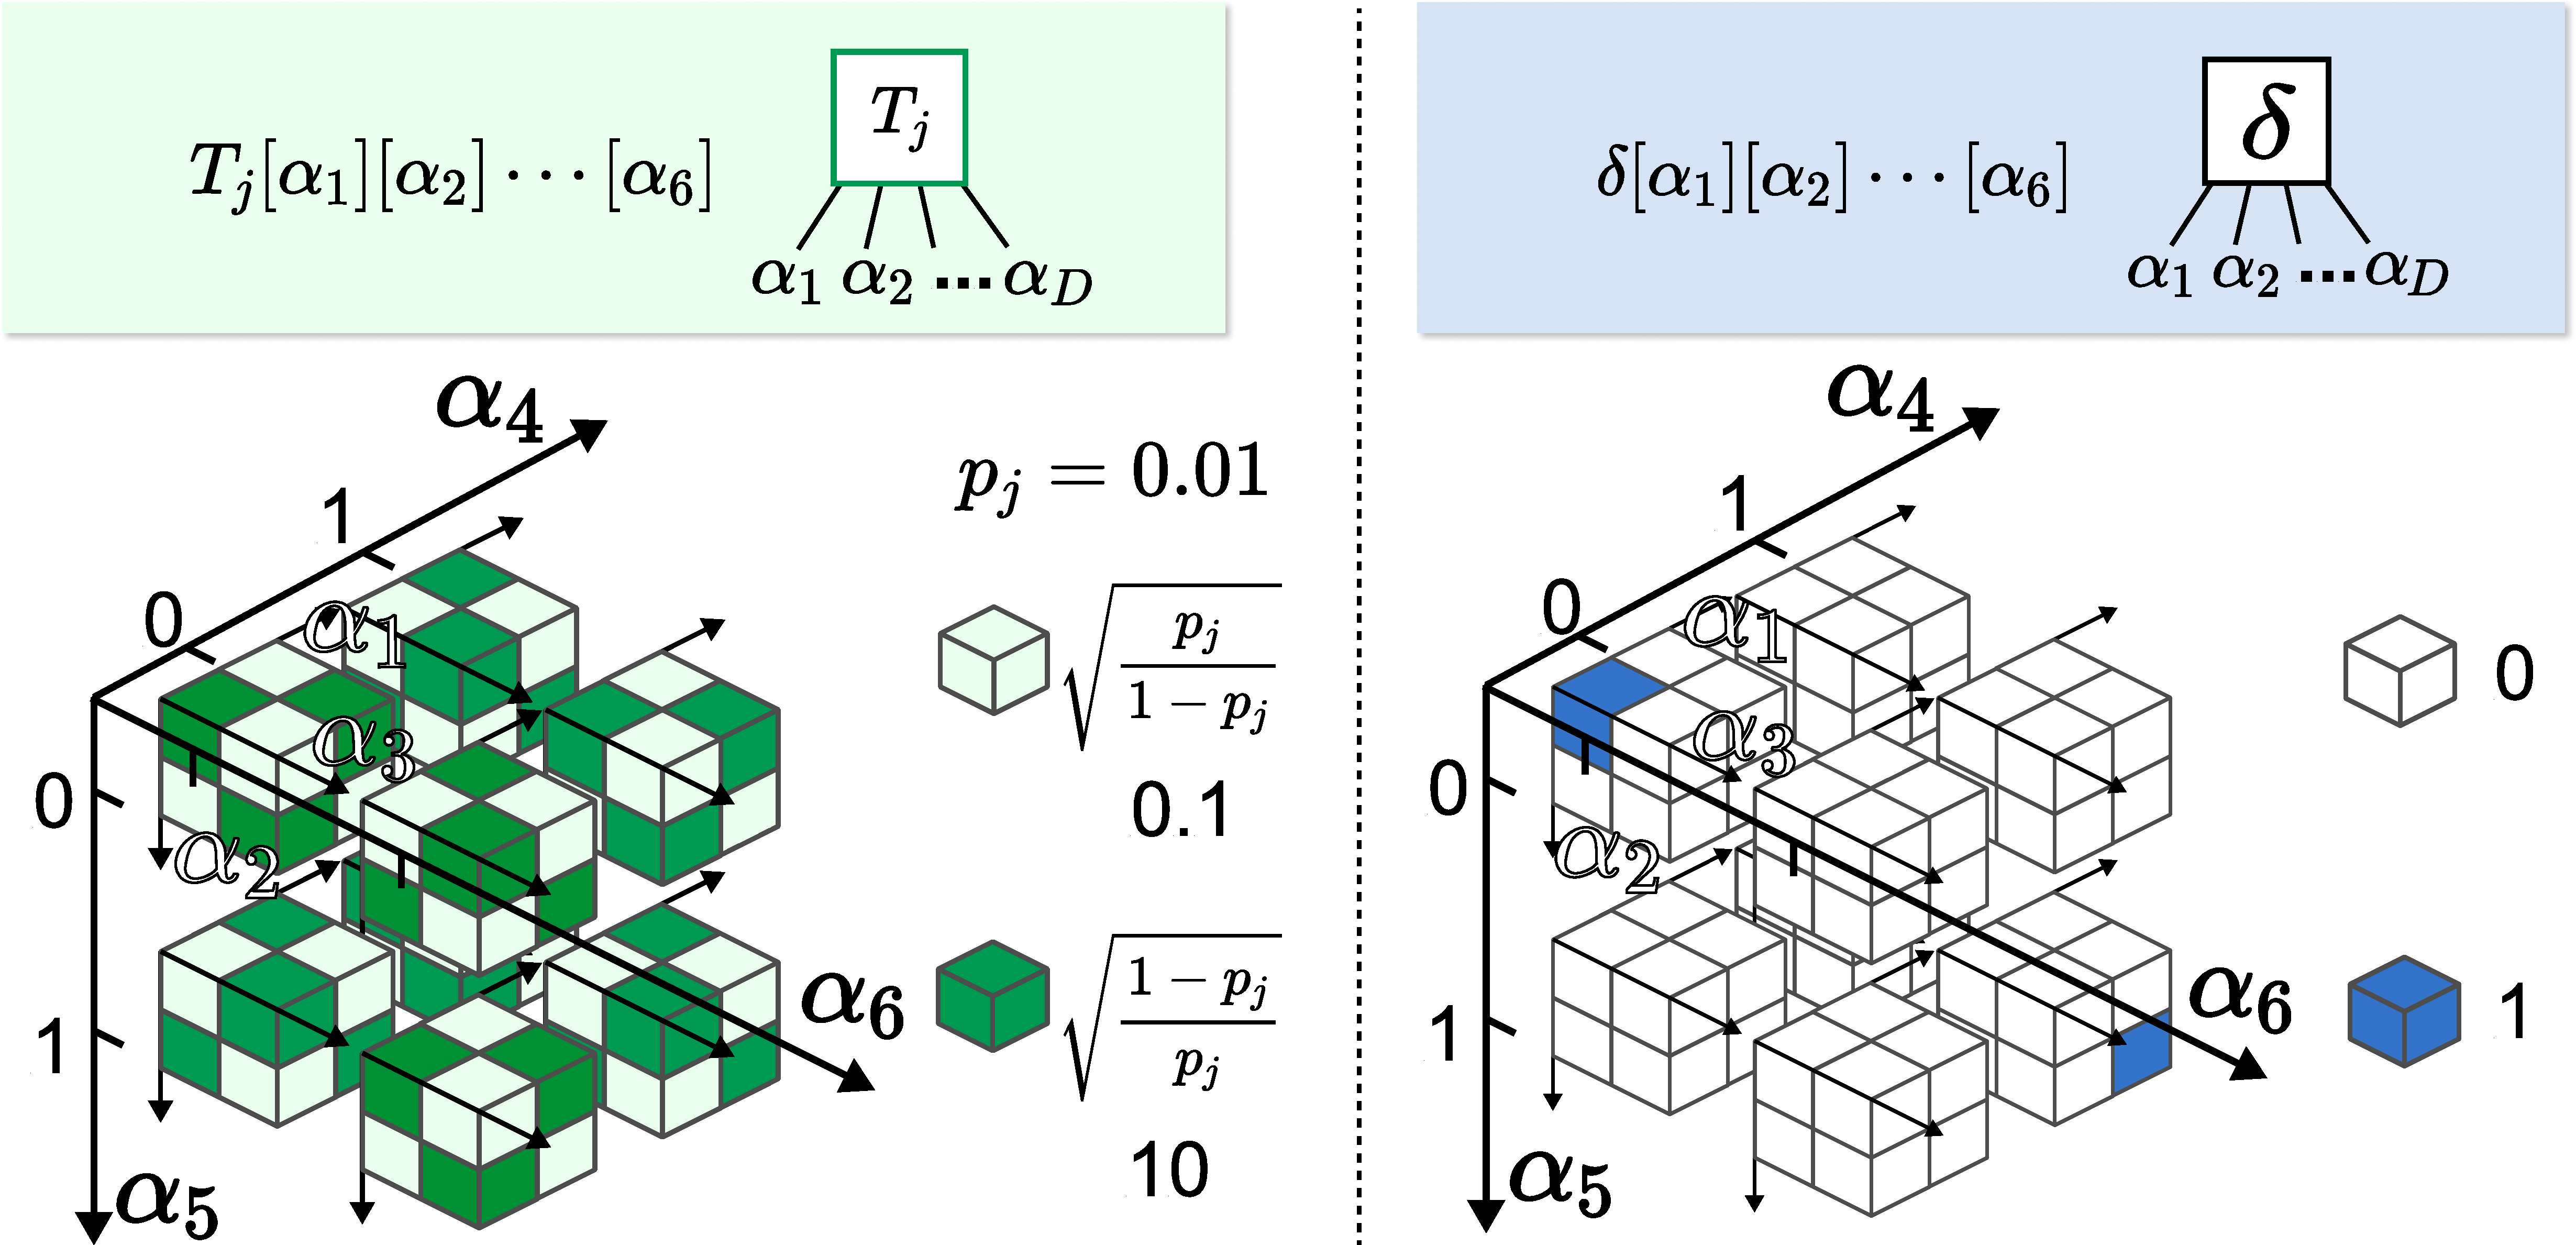
\includegraphics[width=1\columnwidth]{figures/TensorExample.pdf}}
\vspace{-0.3cm}
\caption{The numerical example of the tensors used in the tensor network decoder.} 
\label{fig:tensor_example}
\end{figure}

\subsection{Exact Tensor Decomposition via Matrix Product State}

The raw tensor network involves n-rank tensors with $2^n$ elements, leading to huge computation cost and memory bottleneck. Prior compression techniques often employ singular value decomposition to decompose the tensors into low-rank matrix product states (MPS) or tree tensor network states~\cite{pan2020contracting,ma2024approximate}. However, this coarse-grained decomposition only saves the top largest singular values of tensors and drops the other singular values, causing a significant accuracy loss.

% The tensors in the original tensor network, as shown in \autoref{fig:formulation}~(c), are high-rank tensors with $2^n$ elements, making the contraction suffer from high computation cost and memory bottleneck. Prior work on tensor network contraction using singular value decomposition to decompose the tensors into low-rank Matrix Product States (MPS) or tree tensor network states~\cite{pan2020contracting,ma2024approximate}. \hl{This decomposition only saves the top largest singular values of tensors and drops the other singular values, causing an accuracy loss. }
% \hl{why there is a great accuracy loss?}



\begin{figure}[t]
\centerline{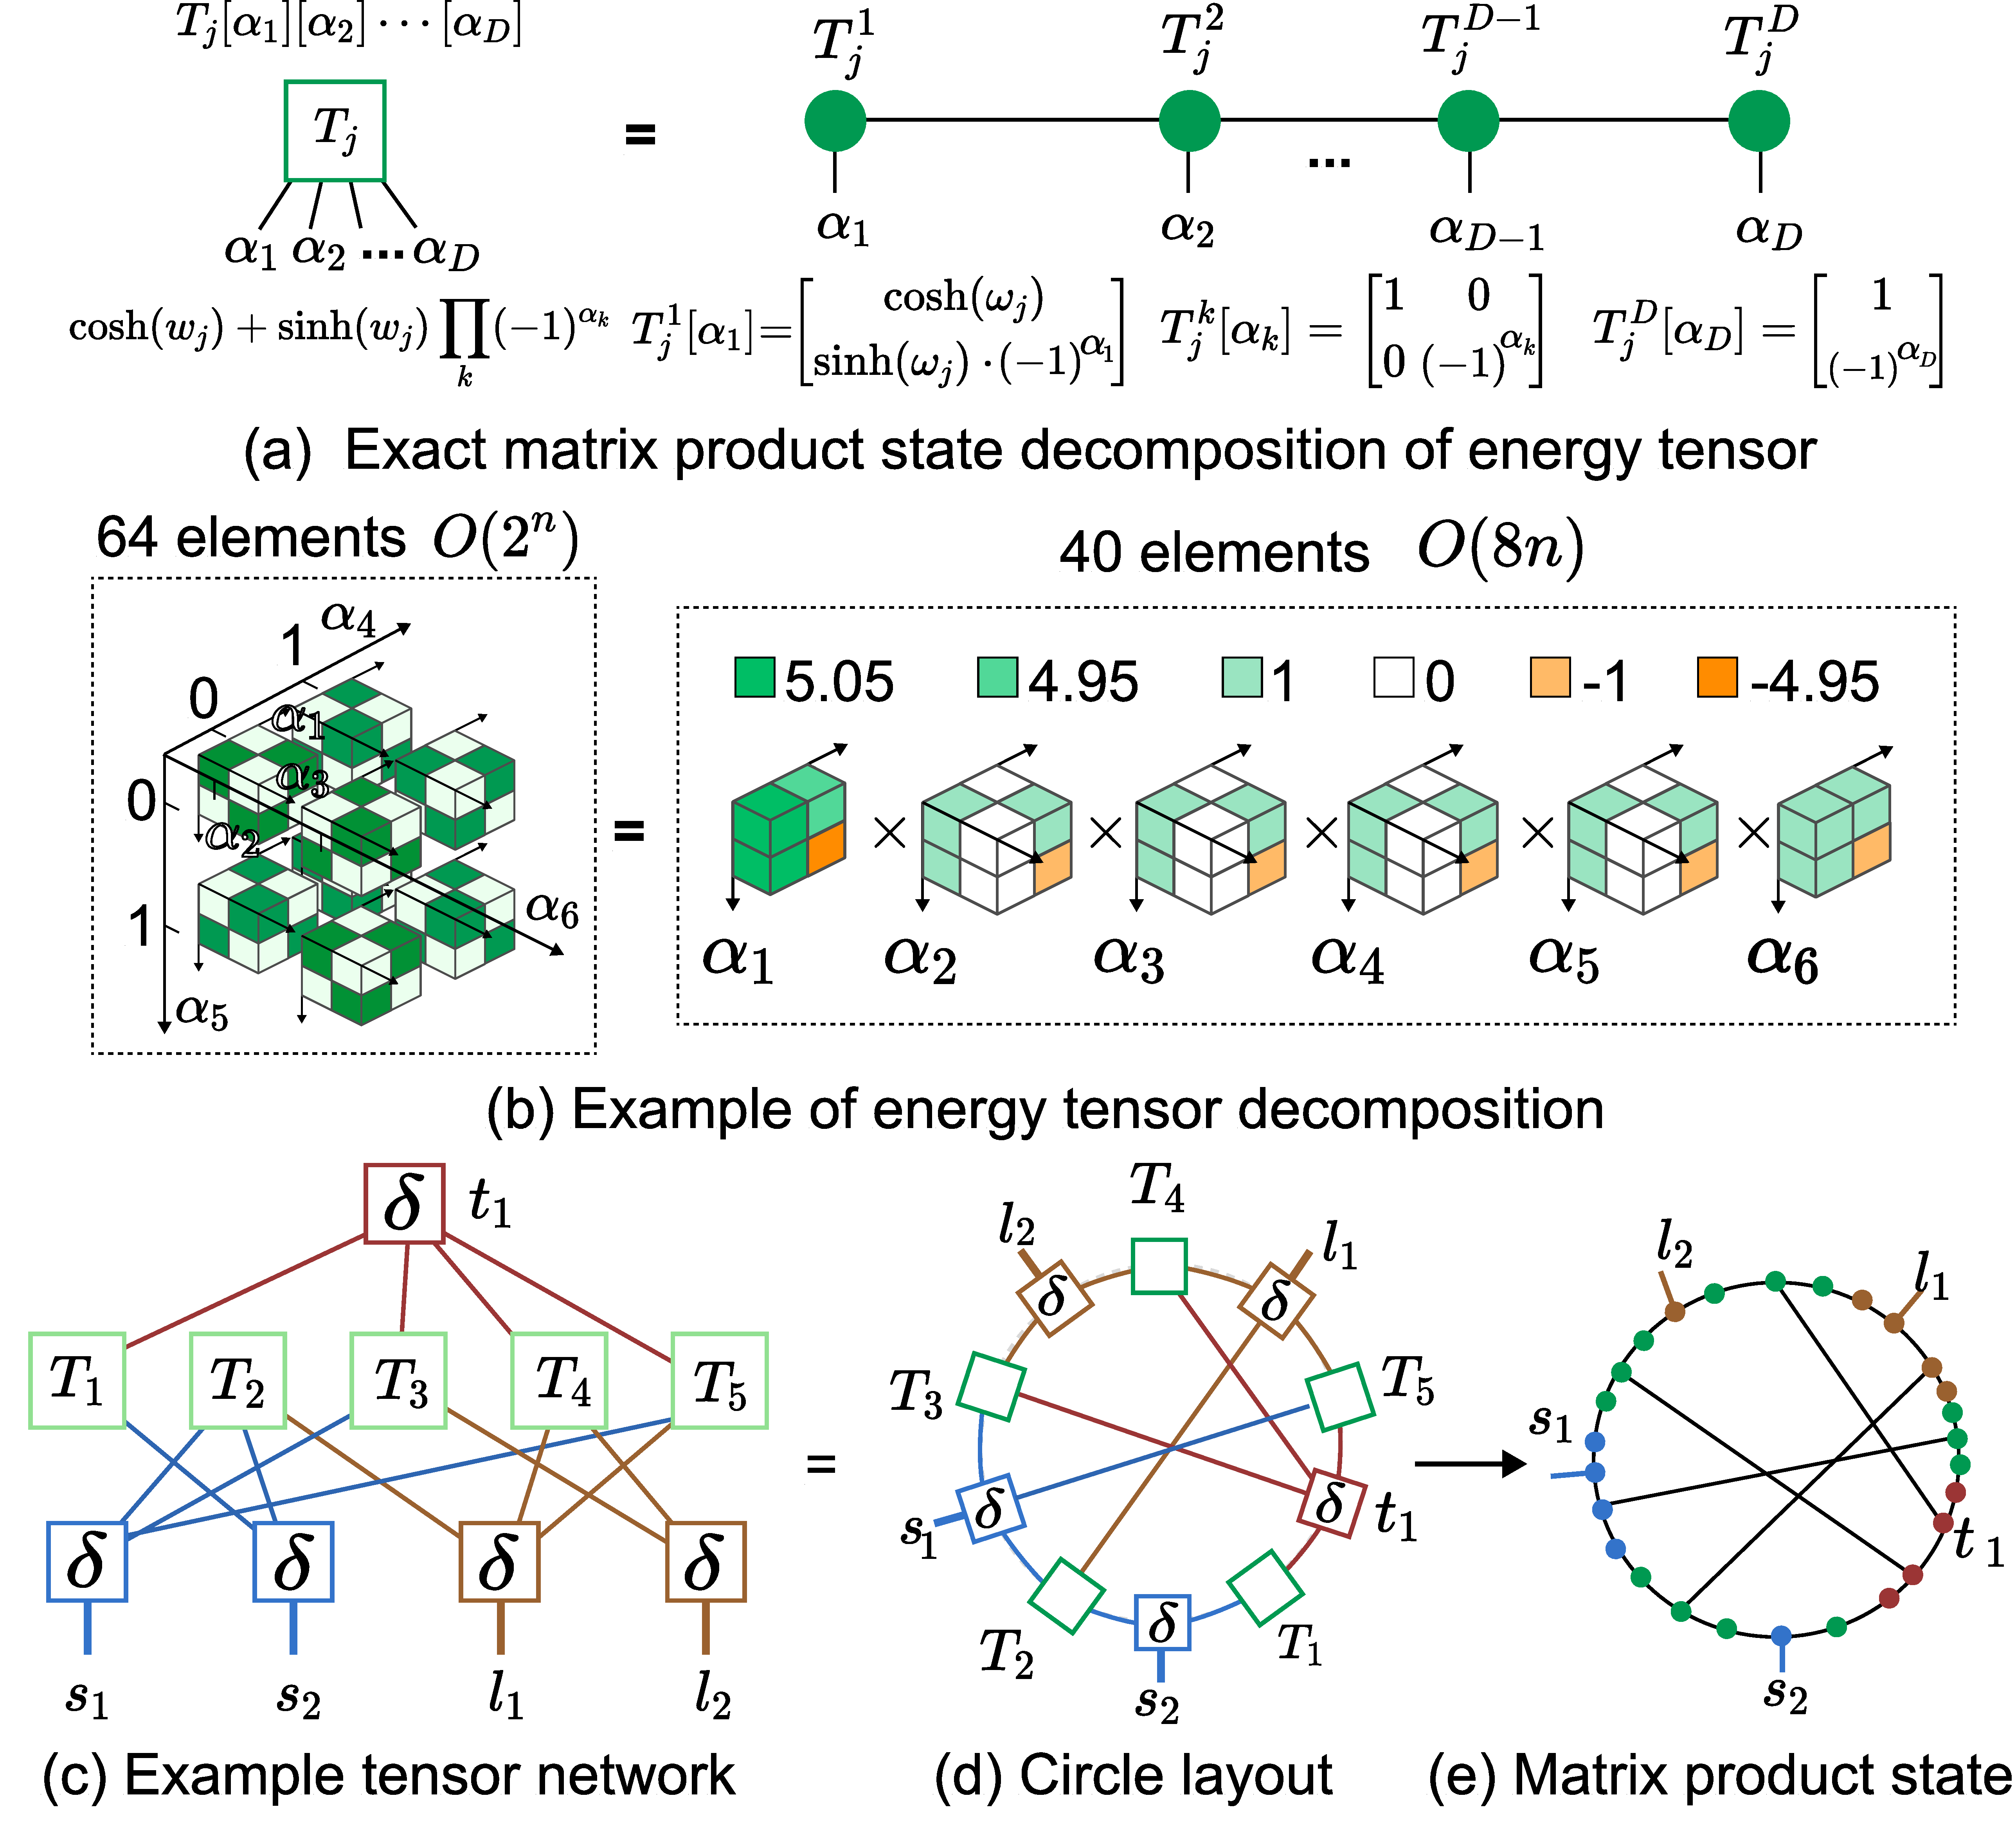
\includegraphics[width=1\columnwidth]{figures/mps.pdf}}
\vspace{-0.3cm}
\caption{Decomposing the tensor network into matrix product states.} 
\vspace{-0.2cm}
\label{fig:mps}
\end{figure}

%先讲讲我们的考虑，我们是怎么想到exact decomposition，为什么我们可以exact，再给具体数学细节
% \hl{insight, motivation, how we got this?}
Considering the binary nature of the errors and check matrices in MLD, we observe that the tensors derived from the spin glass model exhibit a highly structured nature. The pattern includes: 1) each element only has two values (\eqref{eq:tensordelta} and \eqref{eq:tensorTcases}); 2) the same values are in diagonal distribution or interleaved distribution. Identifying these features, we propose an exact decomposition scheme that can equivalently decompose the tensor into a series of smaller matrices, as
shown in \autoref{fig:mps}~(a). 
Specifically, since the results of spin multiplication only have two values, -1 or 1, the tensor can only be $e^{-\omega_j}$ and $e^{\omega_j}$, transforming the tensor $T_j$ in \eqref{eq:tensorT} to hyperbolic functions.
\begin{equation} \small
    T_j = \cosh (\omega_j) + \sinh (\omega_j) \prod_k (-1)^{\alpha_k}
\end{equation}
We can verify that this tensor $T_j$ can be represented by matrix products with the tensors $T_j^k$ in \autoref{fig:mps}~(a).
\begin{equation}\small
    T_j[\alpha_1][\alpha_2]\cdots[\alpha_D] = \prod_{k=1}^{D} T^k_j[\alpha_k]
\end{equation}
\autoref{fig:mps}~(b) gives the example of decomposing a six-rank energy tensor into six three-rank tensors, shrinking the tensor size from 64 elements to 40 elements.
For the tensor $\delta$ in \eqref{eq:tensordelta}, the elements that share the same index $\alpha_k$ have the same values. Thus, it can be exactly decomposed into low-rank tensors $\delta$.
\begin{equation}\small
    \delta[\alpha_1]\cdots[\alpha_D] = \sum_{\vec{\beta}} \delta[\alpha_1][\beta_1] \delta[\beta_1] [\alpha_2] [\beta_2]\cdots \delta[\beta_{D-1}] [\alpha_D].
\end{equation}

\autoref{fig:mps}~(c)-(e) visualizes the tensorization process of the entire tensor network, where the tensor network is derived from \autoref{fig:formulation}~(c). To better understand dimension reduction, \autoref{fig:mps}~(d) organizes it in a circular layout, maintaining the original connectivity. In this circle, we can observe that each tensor is connected with four neighboring tensors at most. By decomposing it into matrix product states, the tensors are converted into three-rank tensors or two-rank tensors, and each has at most three neighbors, as depicted in \autoref{fig:mps}~(e).

% Using the exact matrix product state decomposition, we can represent the original high-rank tensors into two-rank tensors or three-rank tensors, reducing the memory complexity from $O(2^n)$ to $O(8n)$. For instance, the tensor network in \autoref{fig:mps}~(b) contains ten tensors with four-rank at most. If we organize it in a circle layout as shown in \autoref{fig:mps}~(c), we can see that the tensors in the graph show a high-dimensional connection with four neighboring tensors at most. By decomposing it into matrix product states, the tensors are converted into three-rank tensors or two-rank tensors, and each has at most three neighbors, as depicted in \autoref{fig:mps}~(d).






\subsection{Tensor Network Compression by Offline Contraction}

Although MPS partially addresses the computational pressure, especially the memory bottleneck, there remain tremendous computations arising from the high-dimensional connections among matrices. A natural idea is to compress the connectivity offline and introduce a low-dimensional topology MPS when online decoding. Observing that the high-dimensional connection basically results from the internal edges in the circle, as shown in \autoref{fig:mps}~(d), our intuition is to eliminate these internal edges. To achieve this goal, we propose the \textit{contraction-swap-merge} method, which iteratively contracts the small tensors, swaps the tensor indices to put the internal edges in adjacent positions, and merges these edges. These three operations used in this method are defined as follows.
% \hl{three operator.}
\begin{itemize}
    \item The \textit{contract} operation is the basic operation in the tensor network, which merges two adjacent tensors into a new tensor by contracting the edge index between them, as shown in \autoref{fig:operations}~(a). The cost of \textit{contract} operations between two tensors with $d_1$ dimensions and  $d_3$ dimensions is $O(d_1d_2d_3)$, where $d_2$ is the bond dimension between them (The bond dimension is the dimension of the multiplication between two tensors). 
    
    \item The \textit{swap} operation is defined as swapping the two adjacent indices in MPS, such as the $\alpha_2$ and $\alpha_3$ indices in \autoref{fig:operations}~(b). The \textit{swap} cost differs in two cases. Swapping between pairs like $(T,T)$, $(T,\delta)$,$(\delta,\delta)$ has no cost. However, for other cases, swapping between tensors needs to use a contract operation and singular value decomposition with cost $O(d^6)$. This will introduce accuracy loss due to the singular value decomposition is an approximated Ddecomposition~\cite{ma2024approximate}. 
    
    \item The \textit{merge} operation uses two contract operations to merge the adjacent edges between two MPS into one edge with a higher dimension. The cost of the \textit{merge} operation comes from the \textit{contract} operation, as shown in \autoref{fig:operations}~(c).
\end{itemize}


% Matrix product state (MPS) solves the memory bottleneck caused by high-rank tensors but still suffers from the high contraction cost due to the high-dimensional connections between matrix product states, making the deployment on a real-time hardware decoder impractical. A natural idea is to reduce the dimension of the connection topology offline and use a low-dimensional topology matrix product state for online decoding. We further identify that the high-dimensional connection is due to the additional connection edges between each tensor, such as the edges inside the circle in \autoref{fig:mps}~(c). Our intuition is to eliminate these entanglement edges and obtain a tensor network with only tensors on the circle, which is exactly a 1D-chain matrix product state that can be efficiently stored and contracted. To execute this strategy, we designed a \textit{swap-merge-contraction} method. 


\begin{figure}[t]
\centerline{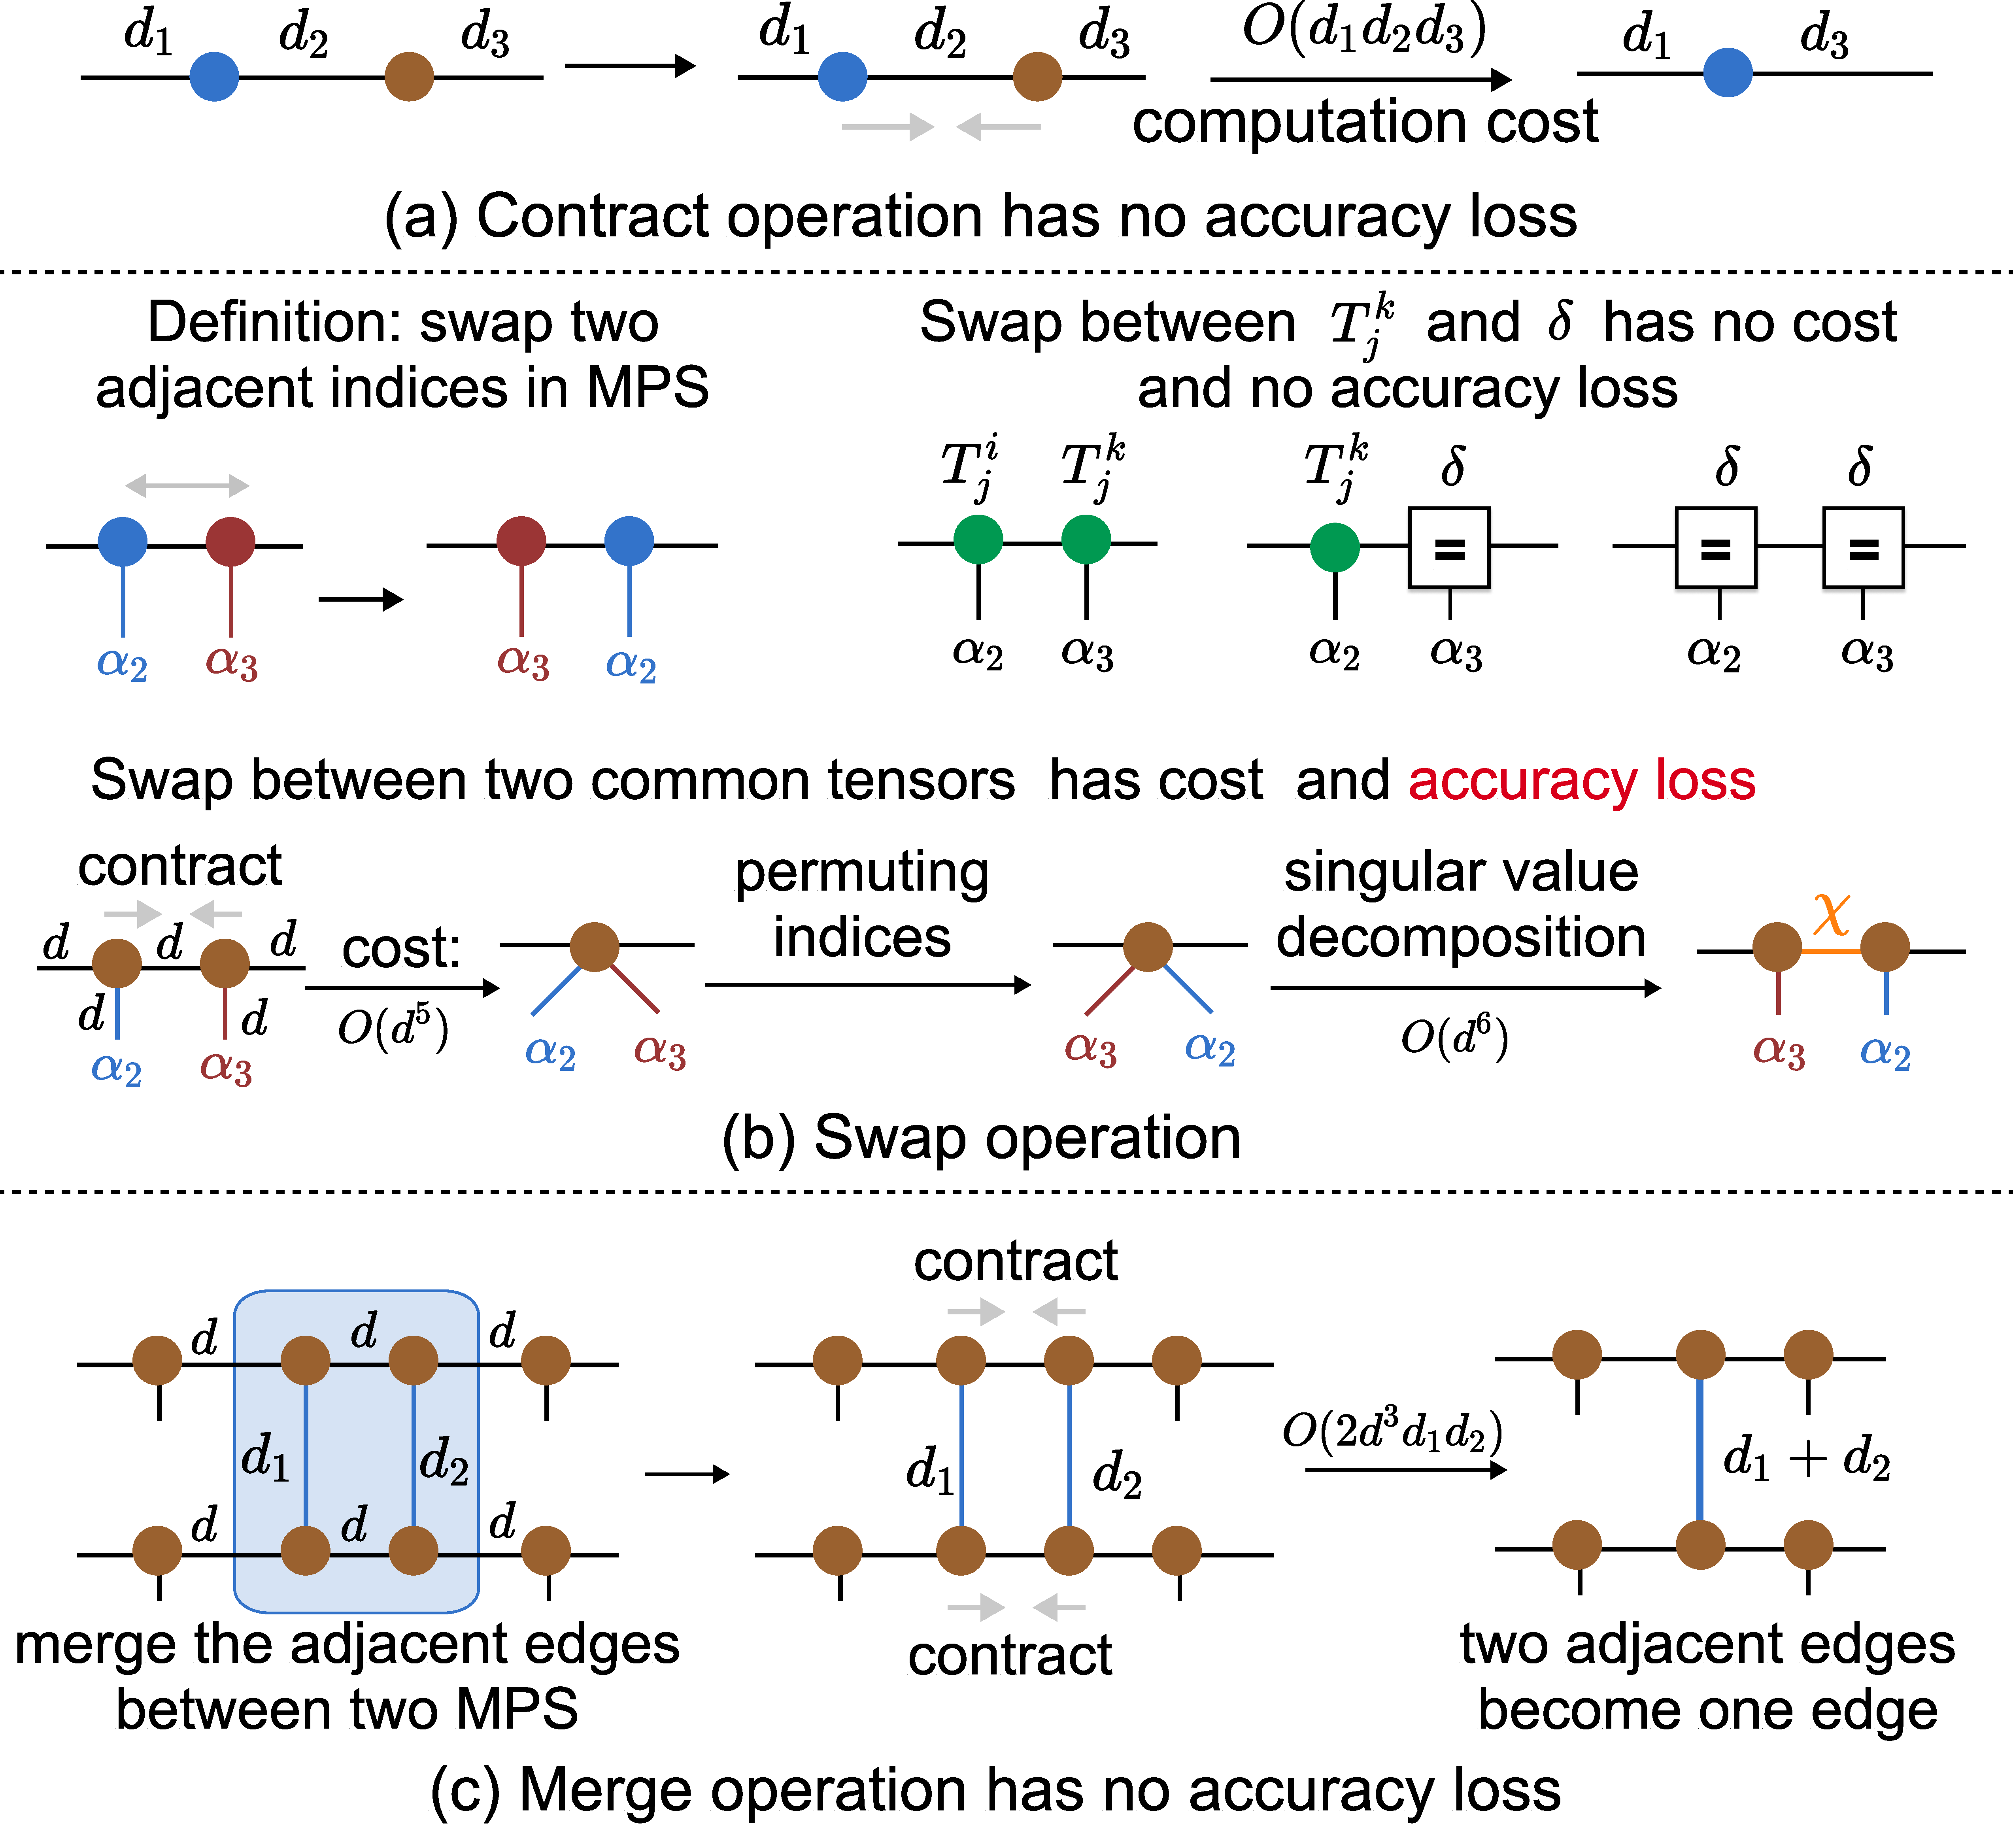
\includegraphics[width=1\columnwidth]{figures/operations.pdf}}
\vspace{-0.4cm}
\caption{Operations definition and cost in offline contraction.} 
\vspace{-0.4cm}
\label{fig:operations}
\end{figure}

\begin{algorithm}[t]
\small
\caption{Contraction-swap-merge Algorithm} \label{algo:contraction}
\KwIn{Tensor network with tensors \( A^{(1)}, \dots, A^{(n)} \), connectivity Tanner graph \( G(V, E) \), set of tensors with outer logical and syndrome indices \( P \subseteq V \)}
\KwOut{1D-chain MPS containing tensors in \(P \)}
Exactly decompose every tensor to MPS\label{line:decompose}\;
\While{\( \exists v \notin P \)}{\label{line:while}
    Find edge \( (i, j) \gets \arg\min_{(\mu, \nu) \in E, \{ \mu, \nu \} \not\subseteq P}  \) \( [ \sum_{b \in \partial \mu} \log(D_{b,\mu})  + \sum_{b \in \partial \nu} \log(D_{b,\nu}) - 2 \log(D_{\mu,\nu})] \) \label{line:argmin}\;
    Move tensor at edge \( (i, j) \) in \( A^{(i)} \) to MPS tail \label{line:move_tail}\;
    Move tensor at edge \( (i, j) \) in \( A^{(j)} \) to MPS head \label{line:move_head}\;
    \textit{Contract} edge \( (i, j) \) to combine MPS \( A^{(i)} \) and \( A^{(j)} \) into a new MPS\label{line:merge}\;
    Update \( E \gets E \setminus \{(i, j)\} \) \label{line:remove_edge}\;
    \For{\( k \in \partial j \)}{\label{line:for}
        Remove \( (j, k) \) from \( E \) \label{line:remove_jk}\;
        \eIf{\( k \in \partial i \)}{\label{line:if}
            \textit{Swap} to place duplicate edges \( (i, k) \) adjacent in \( A^{(i)} \) \label{line:swap}\;
            \textit{Merge} adjacent tensors, combining edges to increase \( D_{k,i} \) \label{line:merge_tensors}\;
        }{
            Add \( (i, k) \) to \( E \) \label{line:add_edge}\;
        }
    }
    \eIf{\( j \in P \)}{
        Add \( i \) to \( P \) \label{line:add_p}\;
    }{
        Update \( V \gets V \setminus \{j\} \) \label{line:remove_node}\;
    }
}
\Return the 1D-chain MPS\label{line:return}\;
\end{algorithm}


% trade-off, algorithm

As we can see, the \textit{swap} operation is an approximation operation with some accuracy loss. Thus, we propose a greedy algorithm to reduce the use of the \textit{swap} operations, as shown in Algorithm~\ref{algo:contraction}. We use a graph \( G(V, E) \) to denote this tensor network, the node \( V \) representing the tensors and edges \( E \) representing the connected indices between tensors $A^{(i)},A^{(j)}$ with a bond dimensions \( D_{i,j} \). The initial bond dimension is 2. Tensors with outer logical and syndrome indices in set \( P \) are preserved, forming a 1D matrix product state chain as output. 
% The edges are contracted iteratively based on minimal cost, preserving outer indices. Bond dimensions exceeding \( \hat{D} \) are truncated via SVD. The process stops when a 1D chain of tensors with outer indices remains, returned as \( Z \).
Specifically, we first decompose the tensors into MPS representation using the exact decomposition (Line \ref{line:decompose}). Then the algorithm loops until all nodes are in the preserved set  \( P \) (Line \ref{line:while}), stopping at a 1D chain. It selects the edge \( (i, j) \) with minimal contraction cost (Line \ref{line:argmin}), moves tensors in \( A^{(i)} \) to the tail (Line \ref{line:move_tail}) and in \( A^{(j)} \) to the head (Line \ref{line:move_head}), then merges them by contracting edge \( (i, j) \) (Line \ref{line:merge}). The edge is removed from \( E \) (Line \ref{line:remove_edge}). For each neighbor \( k \) of \( j \) (Line \ref{line:for}), edge \( (j, k) \) is removed (Line \ref{line:remove_jk}). If \( k \) connects to \( i \) (Line \ref{line:if}), duplicate edges \( (i, k) \) are swapped to be adjacent (Line \ref{line:swap}) and merged, increasing \( D_{k,i} \) (Line \ref{line:merge_tensors}). If \( k \) is not connected to \( i \), edge \( (i, k) \) is added to \( E \) (Line \ref{line:add_edge}). If \( j \in P \), \( i \) is added to \( P \) (Line \ref{line:add_p}); otherwise, \( j \) is removed from \( V \) (Line \ref{line:remove_node}). The final 1D MPS chain is returned (Line \ref{line:return}).

\begin{figure}[t]
\centerline{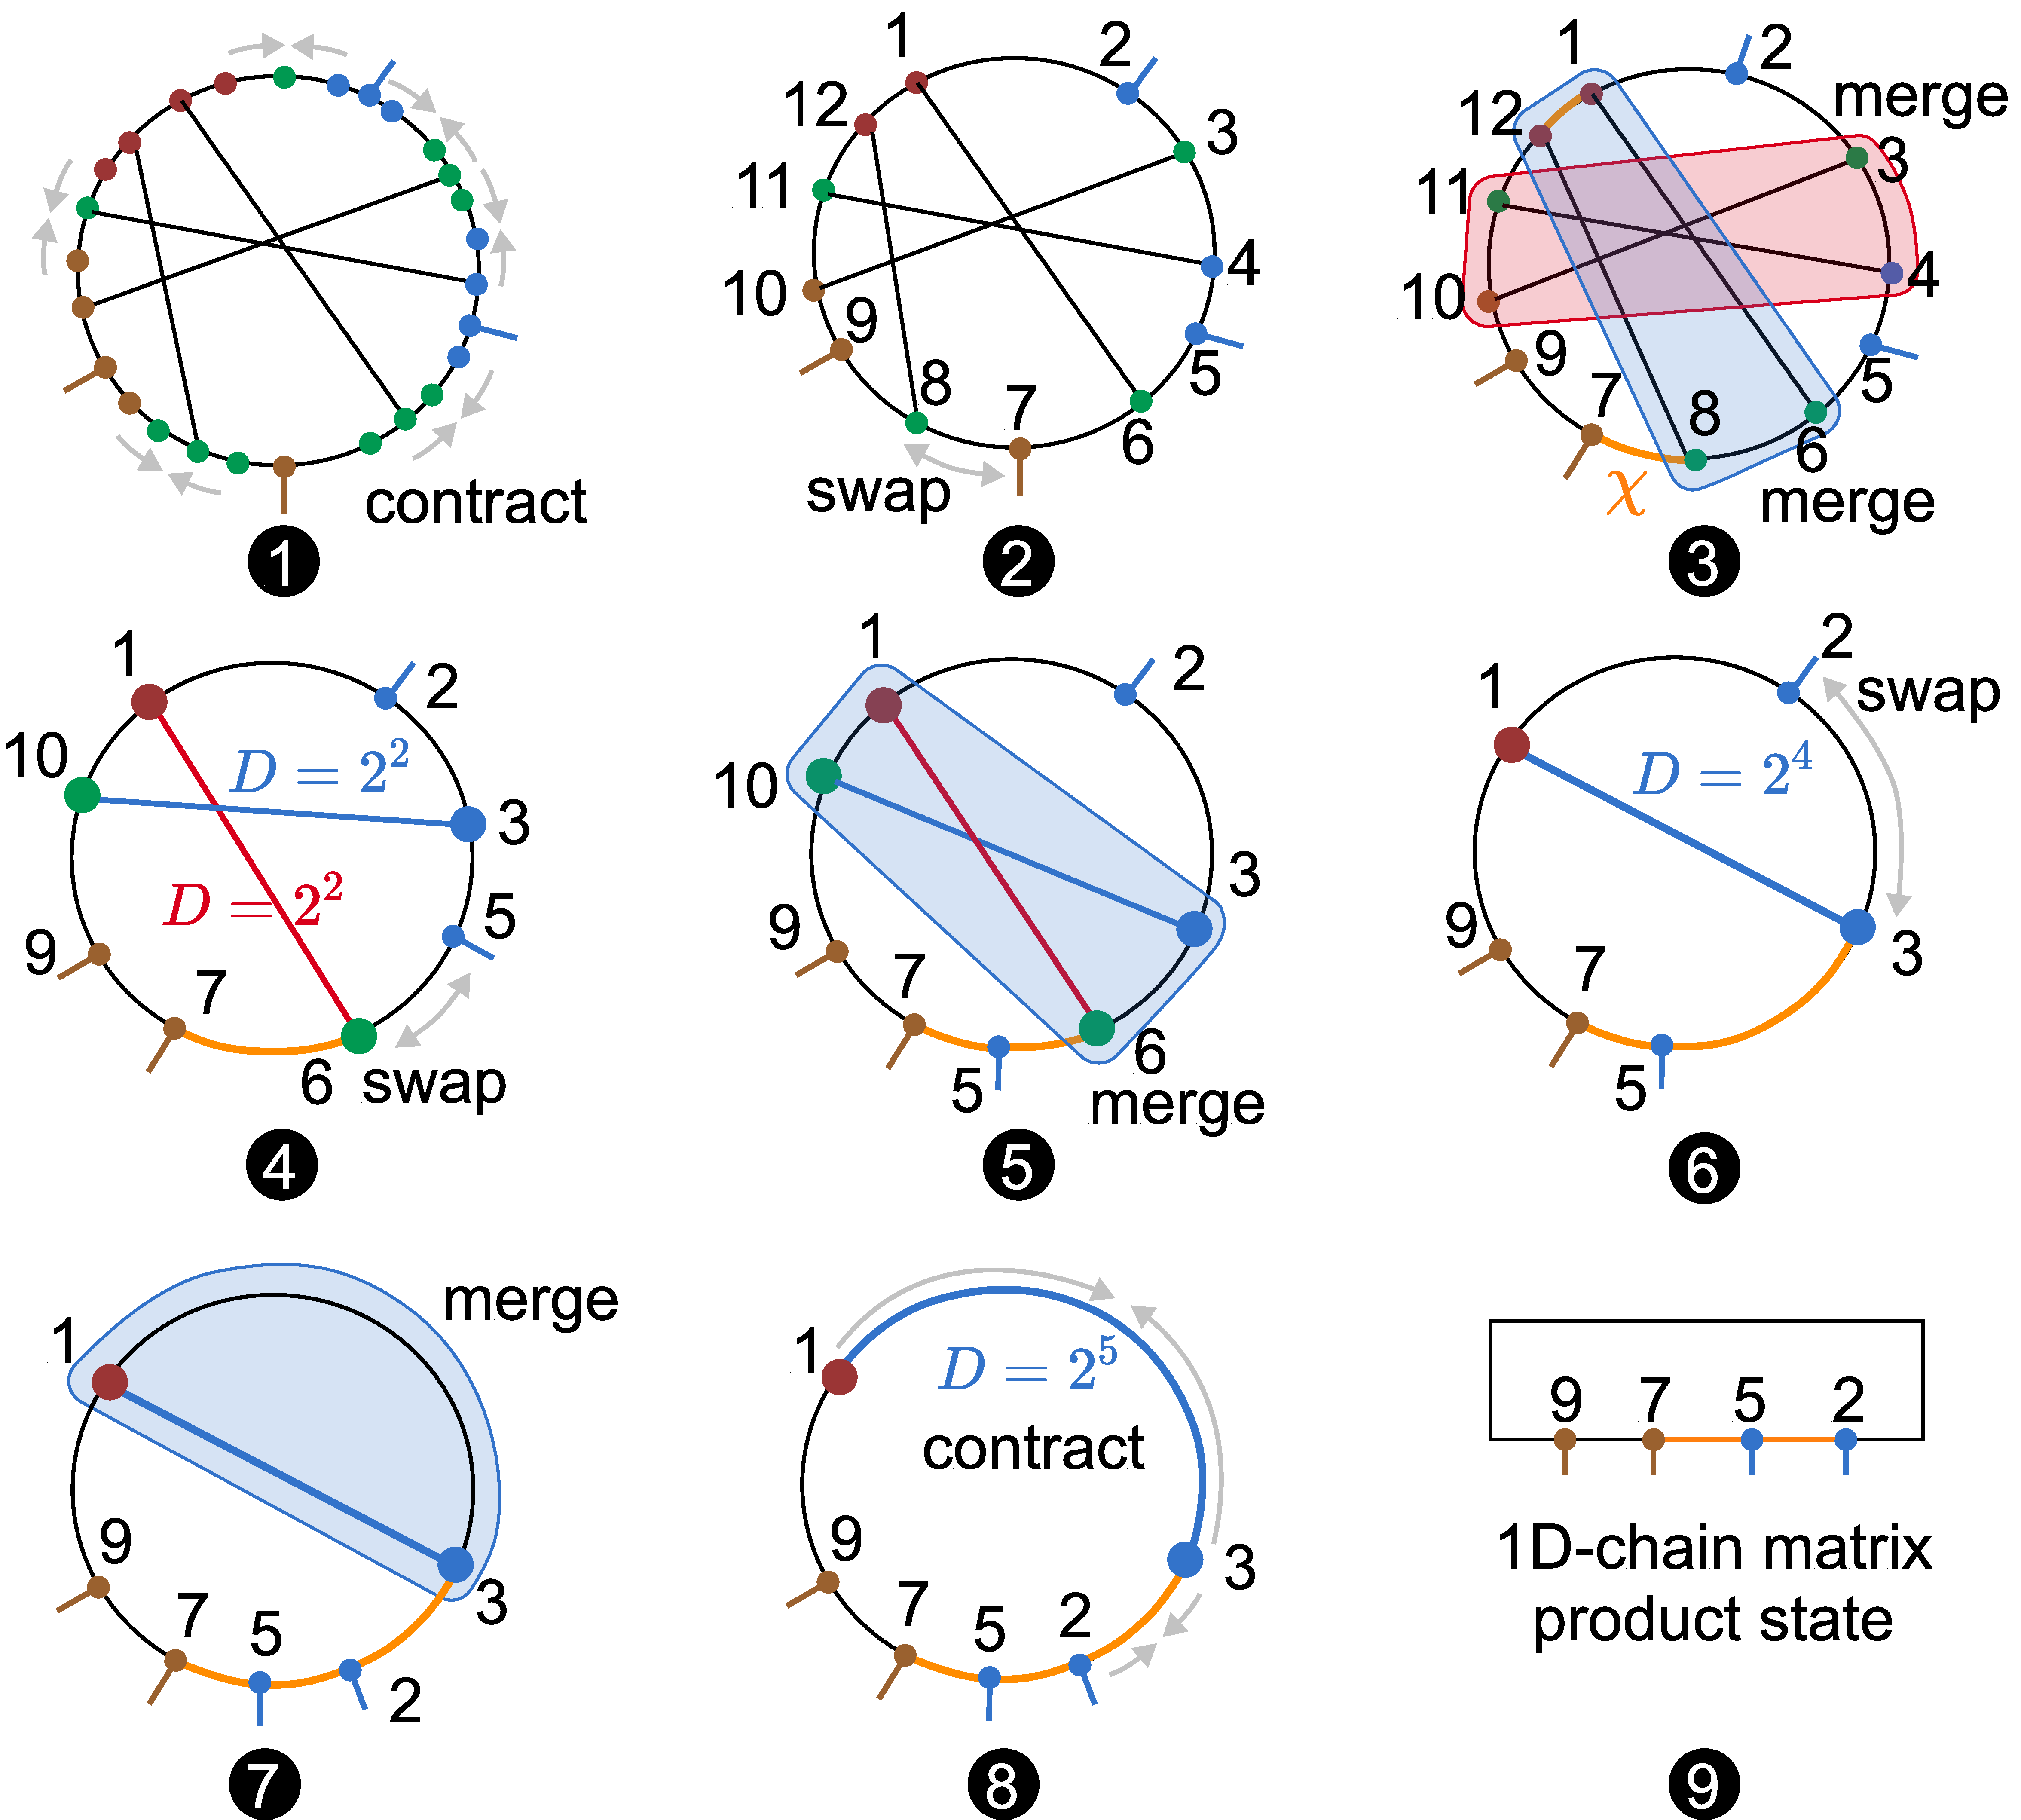
\includegraphics[width=0.9\columnwidth]{figures/circlecontraction9.pdf}}
\vspace{-0.2cm}
\caption{Offline contraction to get the approximated matrix product state for free energies under different syndromes.} 
% \vspace{-0.4cm}
\label{fig:contraction}
\end{figure}



\autoref{fig:contraction} gives an example of the \textit{swap-merge-contraction} approach. We start by \textit{contract} the edges in the MPS representation with the lowest contraction costs as shown in step~\ding{182}. Then we \textit{swap} the two MPS in edge (8,7) as step~\ding{183} to make the two pairs of edges (12,8) and (1,6) in adjacent positions as step~\ding{184}. We \textit{merge} the two pairs of edges \{(12,8) and (1,6), (11,4) and (10,3) \} into two new edges with the bond dimension $D=2^2$ as shown in step~\ding{185}. The steps \ding{185}-\ding{188} also repeat this \textit{swap} and \textit{merge} process until no edges are inside the circle. Then, we \textit{contract} the matrices (1,3) on the circle as in step~\ding{189}, except for the tensors \{9,7,5,2\} with outer logical and syndrome indices, to obtain a 1D-chain MPS with only logical and syndrome indices, as shown in step~\ding{190}.

% 
\section{\papername Decoding Flow and Architecture}

When using the 1D-chain matrix product state for decoding, directly enumerating all logical spins will incur exponential complexity with the number of logical qubits. Thus, we develop a partial tracing strategy to compute the conditional marginal probability of each logical spin in parallel. This strategy takes only $O(M\chi^2+\log K \cdot K^2\chi^4)$ with the number of syndrome checks $M$, the number of logical qubits $K$, and the virtual bond $\chi$  (the dimension of the matrix) of matrix product states, meanwhile maintaining the accuracy of decoding. Based on this polynomial-time decoding flow, we design a dedicated hardware architecture and implement it on the GPU device. We leverage the tensor core for matrix product and the CUDA core for calculating the marginal logical probabilities.

\subsection{Online Decoding via Conditional Marginal Probability}

The 1D-chain MPS contains the free energy under all syndromes and logical spin configurations. The decoding goal is to find the logical spin configuration with minimal free energy when given the syndrome spins. Directly enumerating all logical spin configurations needs $O(2^K(M+K)\chi^3)$, where $K$ is the number of logical qubits, $M$ is the number of syndrome qubits, and $\chi$ is the maximum virtual bond of the 1D-chain MPS.

To overcome the enumeration, we propose to calculate the marginal probability of each logical spin. The marginal probability is computed as 
\begin{equation}\small
    P(l_i=1|\vec{s}) = 
    \frac{{\text{contract}}(\mathcal{T}(l_i=1,\vec{s}))}{\text{contract}(\mathcal{T}(\vec{s}))}. 
    \label{}
\end{equation}
This means we only need to contract the 1D-chain MPS twice under the values of $g_i$ to get the marginal probability. However, using the marginal probability may not determine the value of logical spin $g_i$. For example, when the marginal probability is around 0.5, the value of logical spin can be 1 or -1 with the same probability. To find the most likely logical spin values, we further calculate their conditional probability under the determined spin values. 




\begin{figure}[t]
\centerline{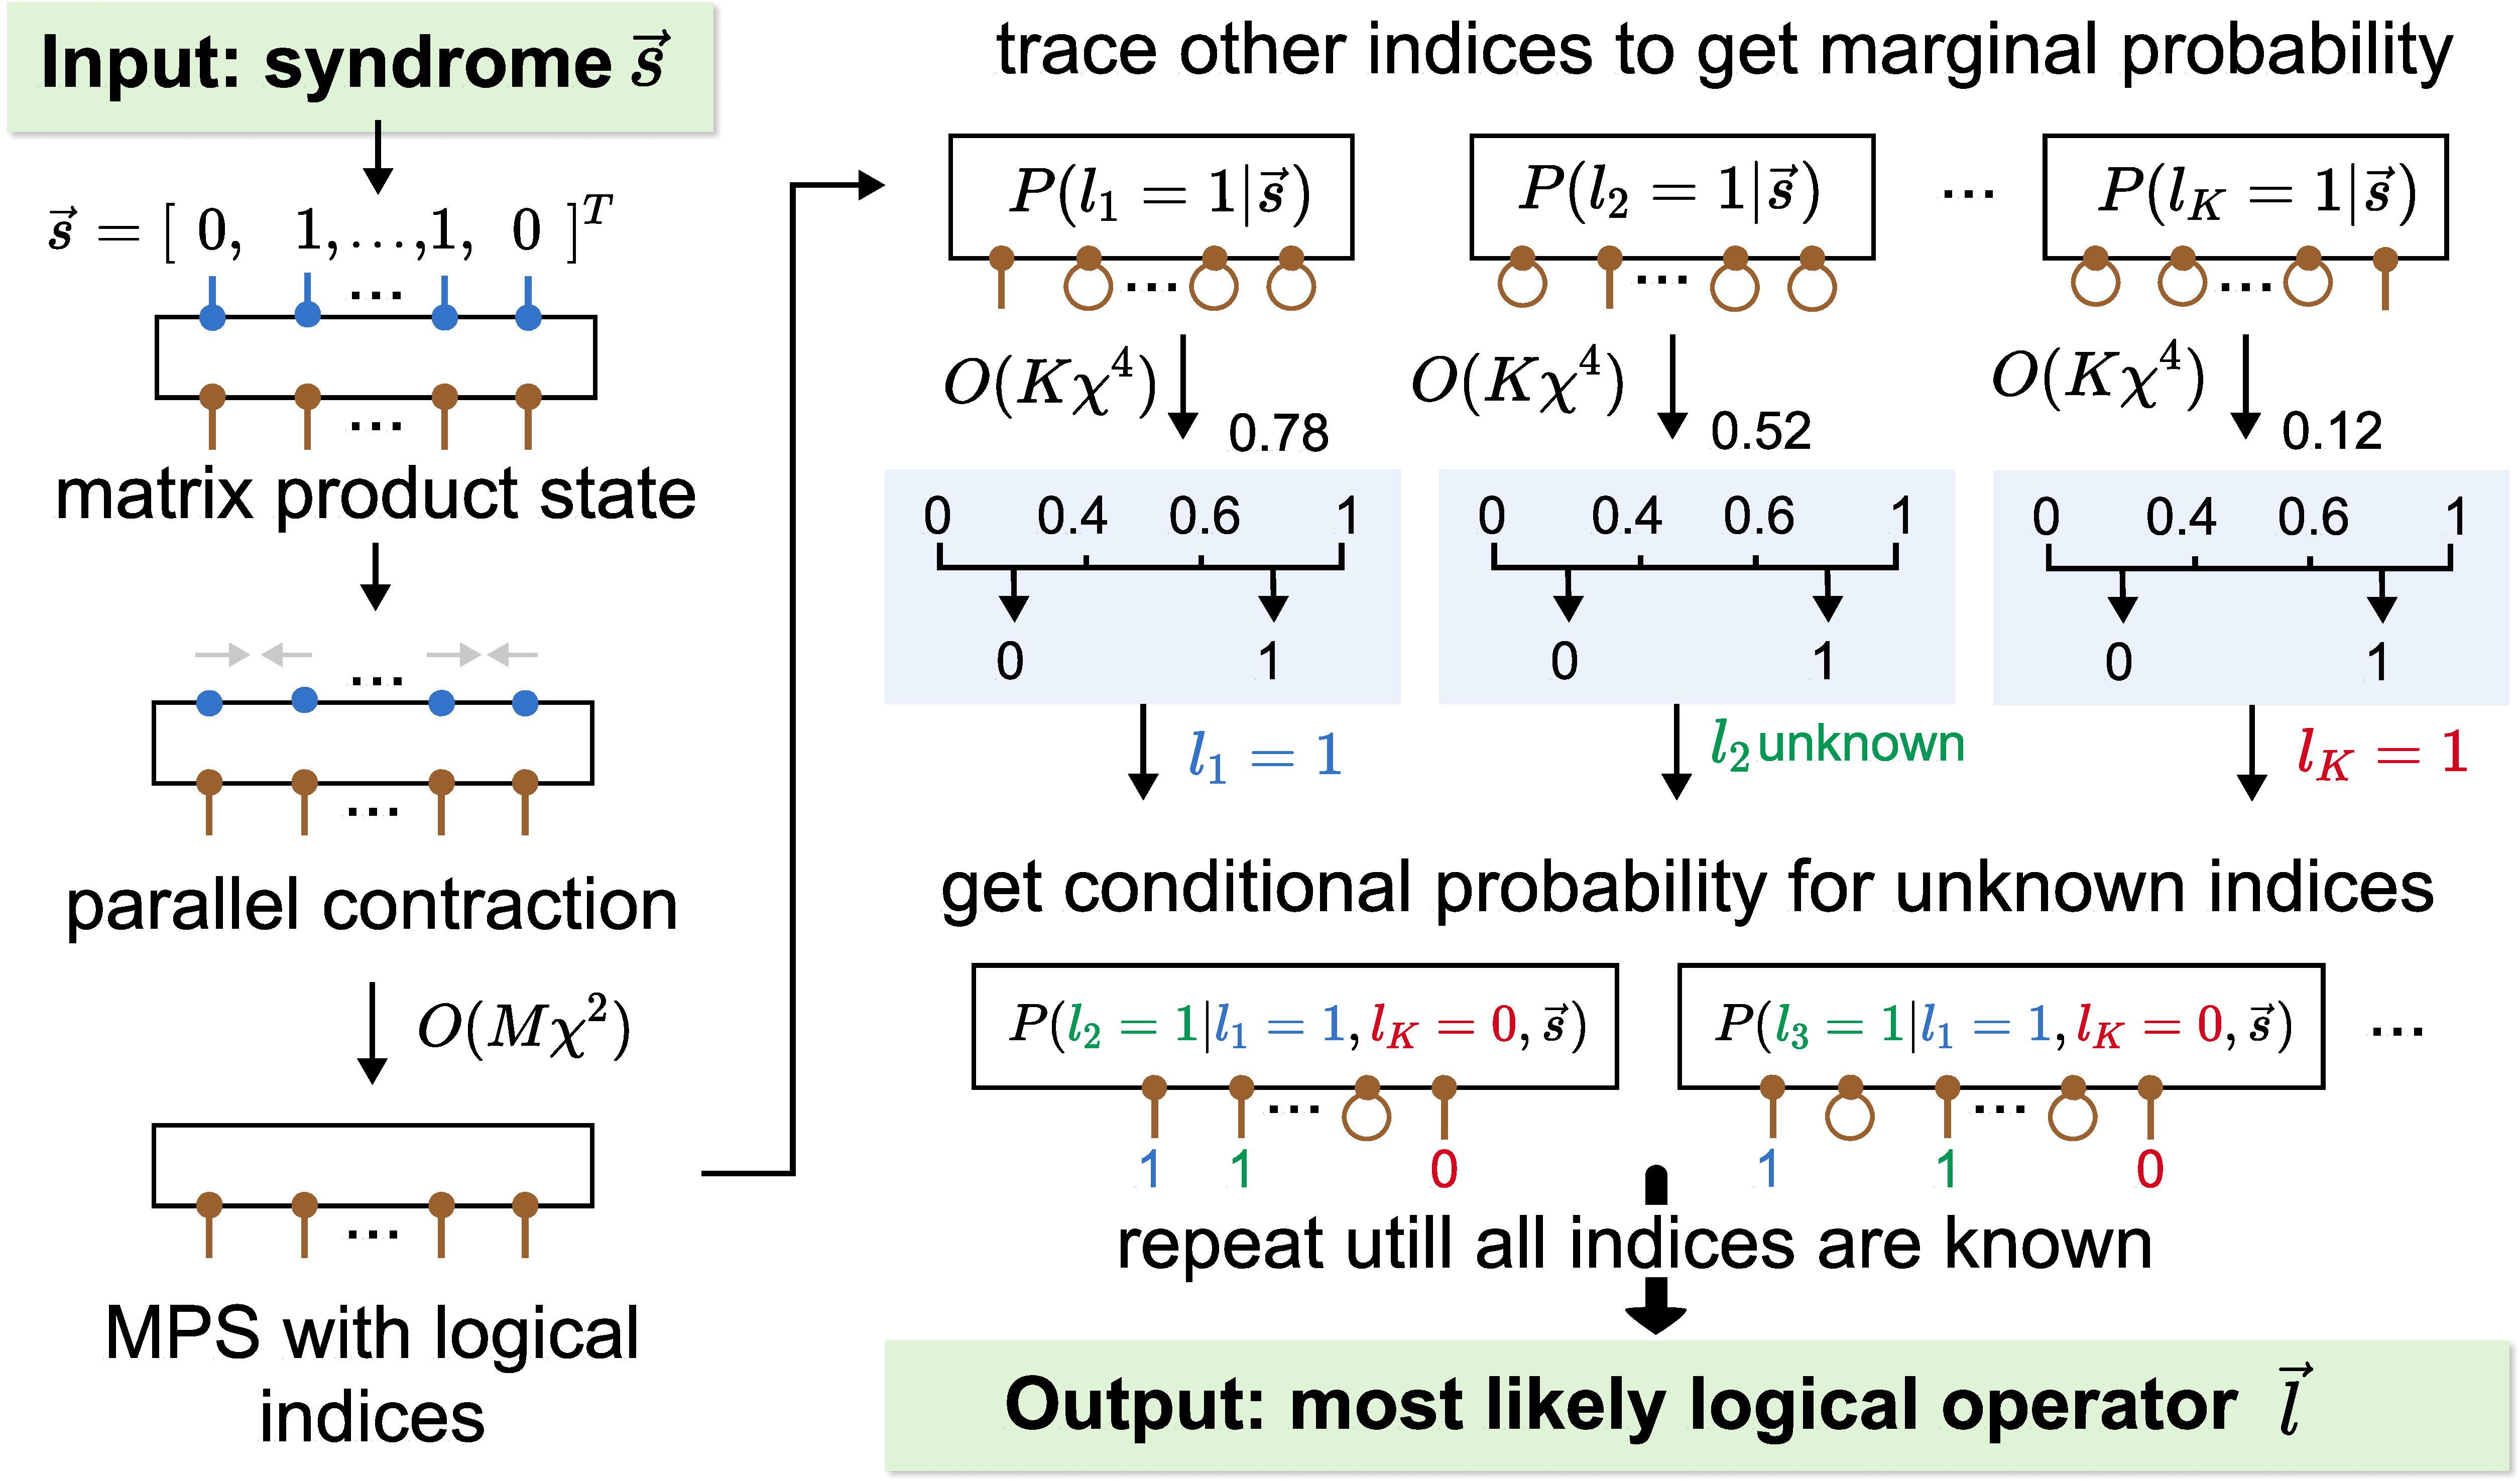
\includegraphics[width=0.98\columnwidth]{figures/logicaldecoding.pdf}}
\vspace{-0.2cm}
\caption{Online decoding via marginal probability calculation.} 
\vspace{-0.4cm}
\label{fig:decoding}
\end{figure}

\textbf{Online decoding flow and complexity analysis}.
\autoref{fig:decoding} illustrates the proposed online decoding flow. The decoder takes the measured syndrome vector $\vec{s}$ as input, representing the outcomes of stabilizer measurements. The MPS e
ncodes the free-energy landscape over all syndrome–logical spin configurations. Given $\vec{s}$, we contract the MPS to obtain one involving only logical spin indices, with a cost of $O(M\chi^2)$, where $M$ is the syndrome length and $\chi$ the maximum bond dimension. To determine the optimal logical spin configuration $\vec{l}$, the marginal probability of each logical spin $l_i$ is computed in parallel by tracing over other indices, requiring $O(K\chi^4)$ computation, where $K$ is the number of logical spins. Spins with probabilities close to 0 or 1 are fixed directly, while ambiguous ones (around 0.5) are refined through local conditional contractions, iterated $O(\log K)$ times. Finally, the recovered logical operator $\vec{l}$ is used to correct the physical state via the~\eqref{eq:recovererror}. This hierarchical contraction strategy reduces complexity from exhaustive enumeration to $O(M\chi^2+\log K\cdot K^2\chi^4)$ sequentially and $O(M\chi^2+\log K\cdot K\chi^4)$ in parallel, enabling scalable decoding.


\subsection{Hardware Architecture of Online Decoding}

\begin{figure}[t]
\centerline{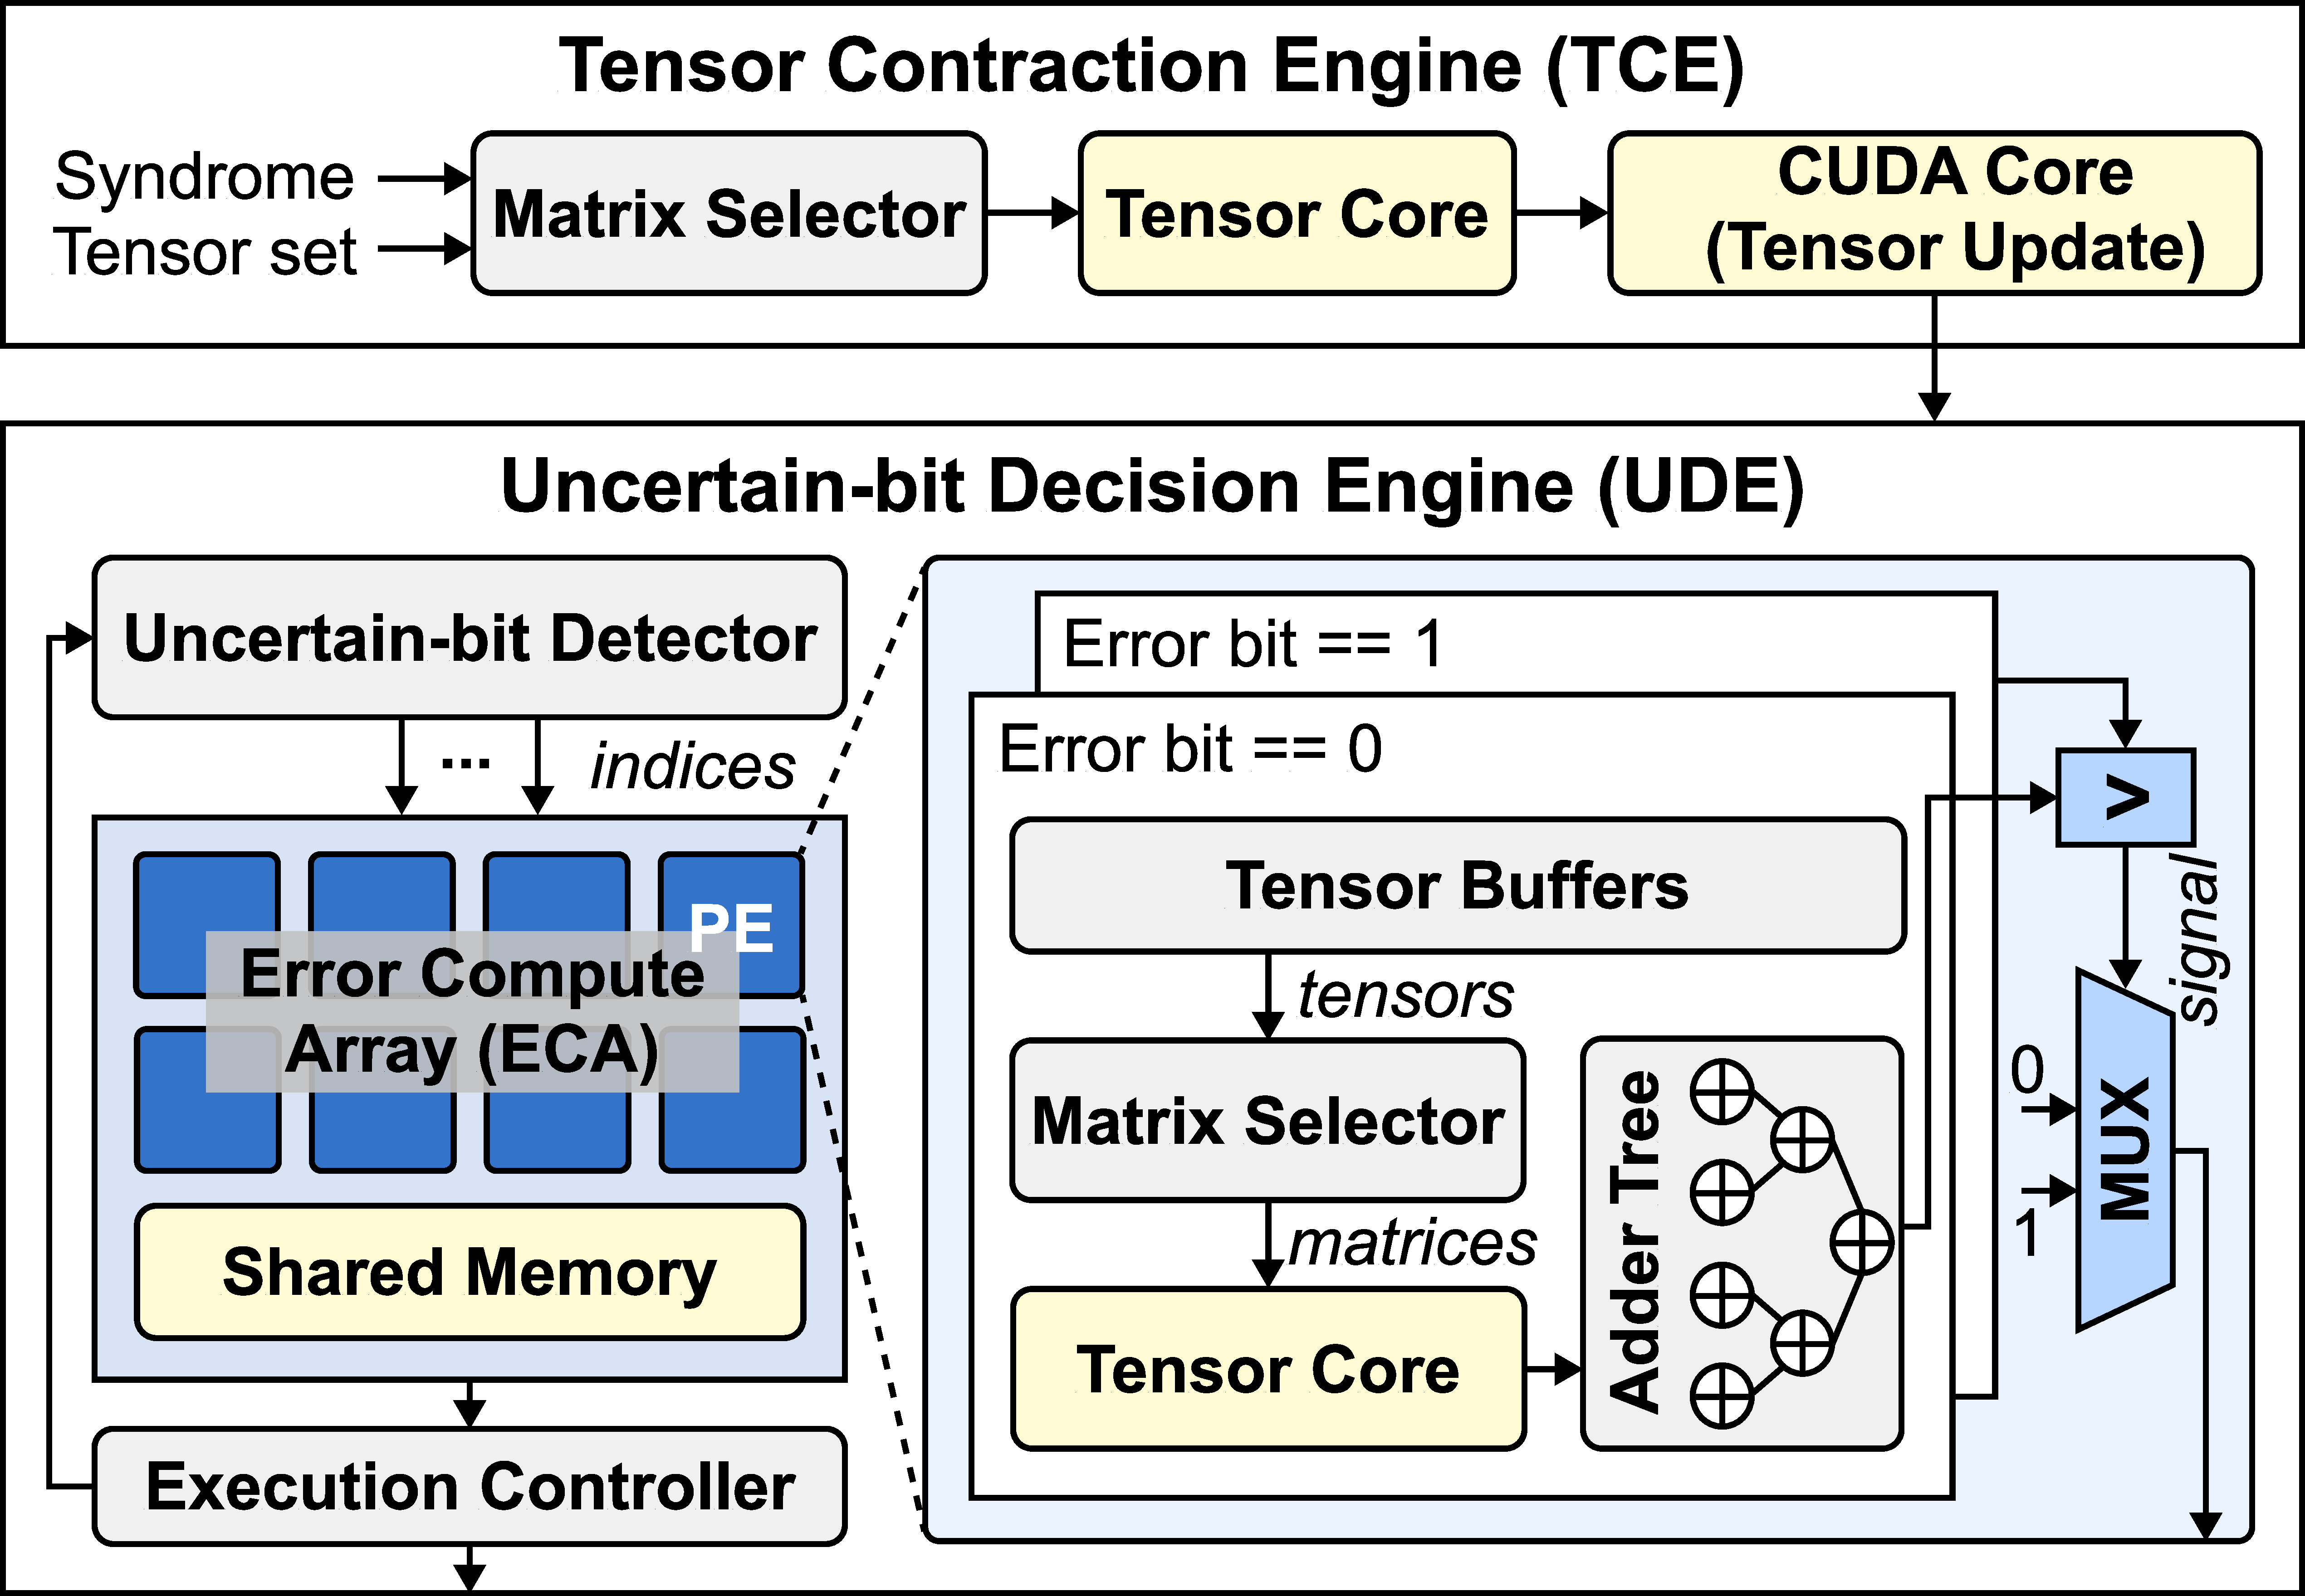
\includegraphics[width=0.95\columnwidth]{figures/gpu_hardware.pdf}}
\vspace{-0.2cm}
\caption{Hardware architecure support for \papername online decoding.} 
\vspace{-0.2cm}
\label{fig:gpu_hardware}
\end{figure}

\autoref{fig:gpu_hardware} presents the \papername hardware architecture designed to support the online decoding computational flow. The architecture consists of two major components: (1) a tensor contraction engine (TCE) and (2) an uncertain-bit decision engine (UDE). The TCE takes the syndrome and the tensor set as inputs. It leverages tensor cores to perform matrix multiplications in parallel and stores intermediate contraction results in shared memory to minimize global memory traffic during iterative tensor updates. A tensor update unit implemented using CUDA cores constructs the 1D-chain MPS with only $K$ tensors and writes them back to the on-chip tensor buffer. Once the MPS chain is generated, it is streamed to the UDE for determining the most probable logical spin configuration.

Within the UDE, an uncertain-bit detector identifies unknown logical indices whose marginal probabilities fall into the uncertainty and dispatches them to the error compute array (ECA). The ECA consists of multiple processing elements (PEs), each dedicated to resolving one uncertain bit. In each PE, the likelihoods for the spin value equal to 0 and 1 are computed in parallel. Specifically, a matrix selector first retrieves the relevant tensors from the on-chip tensor buffers (in shared memory) and feeds the selected matrices to tensor cores. The resulting matrix is then sent to an adder tree implemented by CUDA core–based parallel reductions, which accumulates its diagonal elements to compute the likelihood. Then, we compare the two likelihoods to determine the final value. All uncertain bits are processed in parallel across the PEs to maximize concurrency. Finally, an execution controller monitors whether unresolved bits remain in the logical operator $\vec{l}$. If so, it triggers another round of refinement; otherwise, the decoding process terminates.

% Looking forward, several stages of the pipeline can benefit from FPGA-based design. For example, the tensor update path in the TCE can be mapped to a fully pipelined contraction unit with a scratchpad hierarchy, removing the general-purpose overheads of tensor cores. Likewise, the uncertain-bit detector of UDE matches FPGA spatial parallelism: each PE can be implemented as a hardwired datapath with fixed matrix selection and reduction logic, enabling deterministic per-bit processing. In addition, a lightweight FPGA control engine can orchestrate refinement rounds without GPU scheduling overhead. With these customized modules, the end-to-end latency can be reduced substantially. For instance, a GPU-bound latency on the order of $10^3 \mu s$ can be decreased to sub-$10^1 \mu s$, yielding both higher throughput and better energy efficiency than a pure GPU design.
\section{Evaluation}

%%%%%%%%%%%%%%%%%%%%%%%%%%%% Evaluation Setup %%%%%%%%%%%%%%%%%%%%%%%%%%%%
\begin{figure*}[t]
\centerline{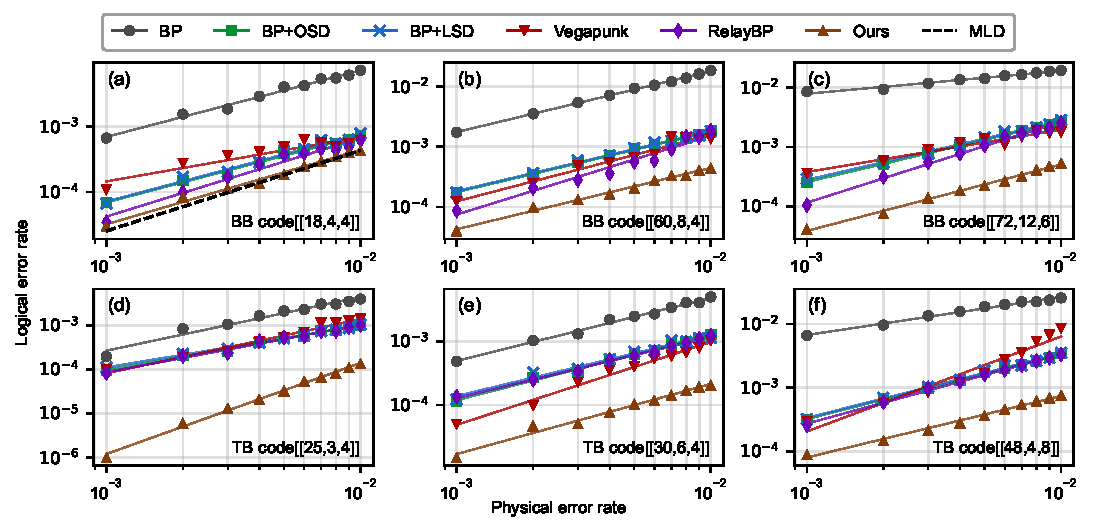
\includegraphics[width=\textwidth]{figures/Evaluation/LER_exp_mld.pdf}}
\vspace{-0.4cm}
\caption{The logical error rates (LER) for BP \cite{bp}, BP+OSD-CS(7) \cite{bposd}, BP+LSD \cite{bplsd}, Vegapunk \cite{zhou2025vegapunk}, RelayBP \cite{relaybp}, \papername, and Exact MLD, respectively. The physical error rate $p$ ranges from $1 \times 10^{-3}$ to $1 \times 10^{-2}$. We evaluate the LER using a depolarizing noise model.}
\vspace{-0.2cm}
\label{fig:LER_exp}
\end{figure*}

\subsection{Evaluation Setup}

\textbf{Metrics.}
We quantify the effectiveness of \papername through three critical performance metrics: (1) the logical error rate (LER), (2) the decoding latency, and (3) tensor compression.
Upon accumulating $d$ rounds of syndromes (where $d$ is the code distance), \papername applies a correction operation to the logical qubit and subsequently measures its state. A logical error happens if this final logical measurement diverges from the pre-initialized state. The decoding process is iteratively executed numerous times under a defined noise model, with each syndrome generated using the Stim package \cite{stim}. The LER, denoted as $p_{l}$, represents the proportion of decoding failures that result in a logical error relative to the total number of trials.
% We can calculate LER per round $p_{r}$ based on the following equation:
% \begin{equation}
%    p_{r} =  1 - (1 - p_{l}) ^ {(1 / d)}
% \end{equation}
% In addition to the LER, we use the fault-tolerant threshold $p_{\text{th}}$ to evaluate the decoder’s tolerance to the physical error rate $p$. Specifically, when the physical error rate $p$ falls below $p_{\text{th}}$, the logical error rate $p_l$ decreases as the code distance $d$ increases. 
% A higher threshold indicates a greater resilience of the decoder to physical noise. The mathematical expression among $p_{r}$, $p$, and $p_{\text{th}}$ can be described as:
% \begin{equation}\small
%  p_r \approx A \left( \frac{p}{p_{\text{th}}} \right)^{\lfloor (d+1)/2 \rfloor}
% \end{equation}
% Here, $A$ is a constant parameter dependent on the code and error model. This tells us that when $p = p_{\text{th}}$, the $p_r$ is equal for different code distances $d$. Therefore, the threshold $p_{\text{th}}$ is determined by the intersection point of the $p_r-p$ curve under different code distances.

\textbf{Baselines.}
We evaluate the decoding performance of \papername against state-of-the-art decoders for qLDPC codes, including belief propagation (BP) \cite{bp}, BP with ordered statistic decoding (BP+OSD) \cite{bposd}, BP with localized statistics decoding (BP+LSD) \cite{bplsd}, Vegapunk \cite{zhou2025vegapunk}, and RelayBP \cite{relaybp}.
For BP, we adopt the min-sum update rule and set the maximum number of BP iterations to the number of data qubits $n$ in qLDPC codes.
For BP+OSD, we adopt the BP+OSD-CS(7) variant, which is known to achieve a good balance between decoding latency and accuracy. The BP part also utilizes the min-sum update rule, and the maximum number of iterations is set to the length of the error vector.
For BP+LSD, we set the maximum number of BP iterations to 30 and the OSD order to 0. We use the sequential version of BP+LSD \cite{Roffe_LDPC_Python_tools_2022}, since no open-source parallel implementation is currently available.
For Vegapunk, we set the maximum iteration of the greedy decoding algorithm to 3, since it offers the best tradeoff between decoding accuracy and latency.
For RelayBP, we set the maximum BP iterations for the first ensemble to 80, the number of relay ensemble elements to 100, and the maximum iterations per relay ensemble to 60.
% All baselines are implemented with an open-source C++ package LDPC v2~\cite{Roffe_LDPC_Python_tools_2022}. 

\textbf{Implementation.}
For the tensor network, we use Quimb 1.11.1~\cite{gray2018quimb} with Python 3.12.1 to evaluate the memory and computation cost of contracting the tensor network. We also use it to implement the offline contraction of the matrix product states. For the online decoding with a 1D-chain matrix product states, we implement it using CuTensorNet 2.8.0~\cite{cuQuantum} with CUDA 12.0. All experiments are conducted on an AMD EPYC 9554 64-core CPU and NVIDIA
A100 80GB GPU. We leverage the fused multiply-add operation in tensor cores for implementing the Tensor Contraction Engine, and use streaming multiprocessors in the GPU to implement the Uncertain-bit Decision Engine.

\textbf{Benchmarks.}
To comprehensively evaluate the performance of the decoder, we conduct experiments on six types of qLDPC codes. We adopt three bivariate bicycle (BB) codes \cite{bbcode}, including [[18,4,4]], [[60,8,4]], and [[72,12,6]], and three trivariate bicycle (TB) codes \cite{voss2025multivariate}, including [[25,3,4]], [[30,6,4]], and [[48,4,8]].

\textbf{Error model.}
We evaluate the performance of decoders using the widely used depolarizing noise model, which assumes each qubit is subject to a depolarizing channel with probability $p$, where $p$ is the physical error rate. This channel transforms an ideal state into a completely mixed state with probability $p$, and leaves it ideal with probability $1-p$. Errors occur independently across qubits.

%%%%%%%%%%%%%%%%%%%%%%%%%%%% Evaluation Results %%%%%%%%%%%%%%%%%%%%%%%%%%%%
\subsection{Logical Error Rate}

\begin{figure}[t]
\centerline{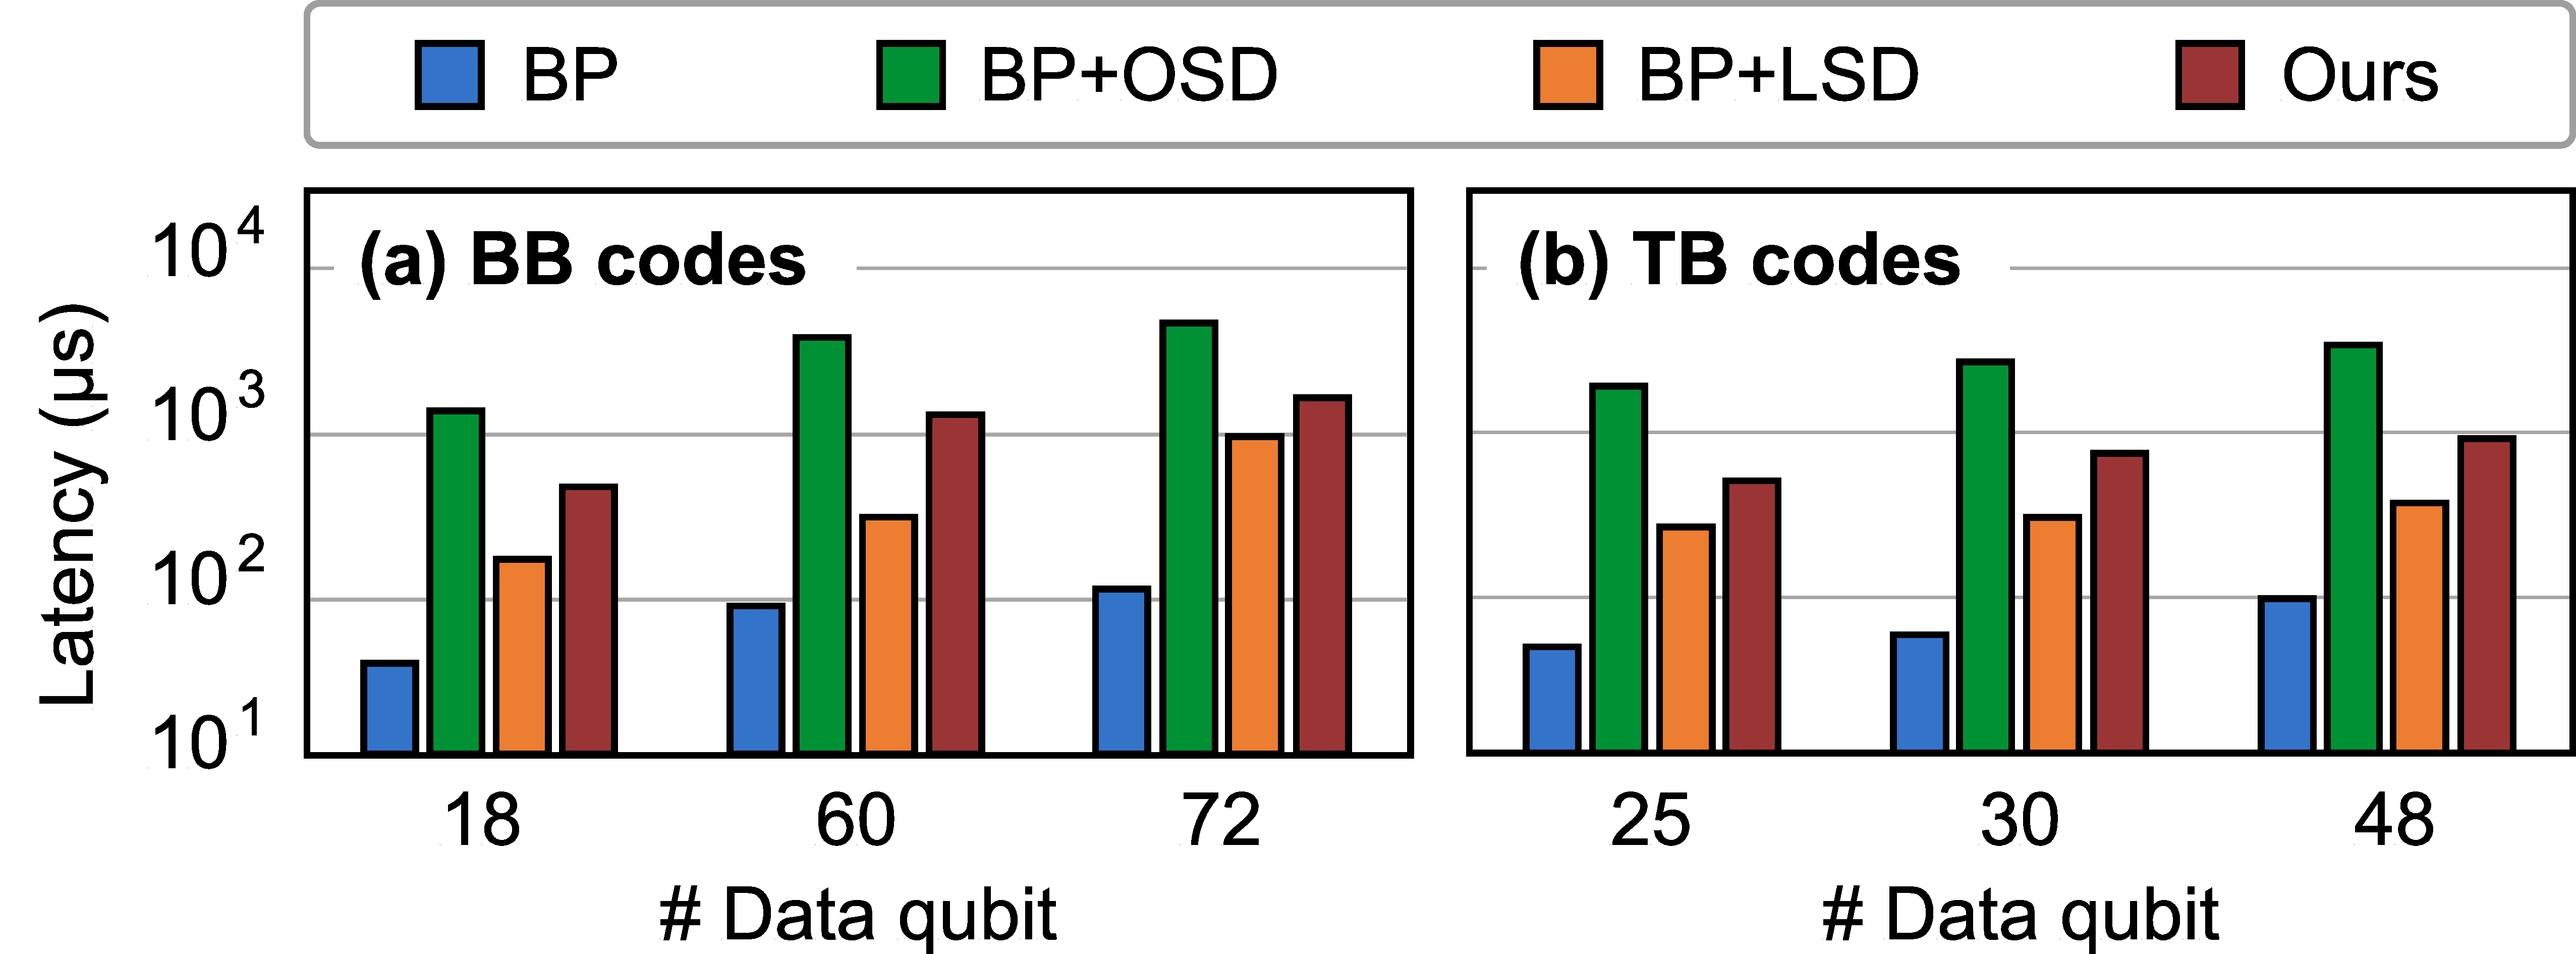
\includegraphics[width=1.0\columnwidth]{figures/Evaluation/latency.pdf}}
\vspace{-0.3cm}
\caption{Decoding latency of BP \cite{bp}, BP+OSD \cite{bposd}, BP+LSD \cite{bplsd}, and \papername on (a) BB codes and (b) TB codes, respectively.}
\vspace{-0.2cm}
\label{fig:latency}
\end{figure}

% \textbf{Logical error rate}.
As shown in \autoref{fig:LER_exp}, \papername reduces $1.55\sim 112\times$ logical error rate compared to prior decoders such as the state-of-the-art BP+OSD decoder. The maximum virtual bond of matrix product states in \papername is set to $\chi=16$. In particular, \papername achieves average $12.5\times$ logical error rate reduction on BB code [[18,4,4]], TB code [[30,6,4]], TB code [[48,4,8]]. Especially in TB code [[48,4,8]], the \papername has a logical error with $10^{-8}$ in physical error rate $10^{-3}$, which is $112\times$ lower than that of BP+OSD decoder.
% We also notice that the BP+LSD has achieved a similar logical error rate to that of BP+OSD, as claimed. The BP decoder has the highest logical error rate, as it often fails to converge due to degeneracy. 
Besides, we observe that the logical error rate curve of \papername has a larger slope than other decoders, which means \papername improved the error suppression capacity of qLDPC codes.

We compare \papername with recent qLDPC decoders, namely Vegapunk \cite{zhou2025vegapunk} and RelayBP \cite{relaybp}. Vegapunk achieves accuracy comparable to BP+OSD and BP+LSD, with higher performance on some codes, such as TB code [[30,6,4]], due to its decoupling strategy and greedy decoding. RelayBP, recently proposed by IBM, outperforms existing baselines through a relay ensembling technique that enhances BP’s robustness against trapping sets. In contrast, \papername delivers an average accuracy improvement of $1.97\times \sim 13.6\times$ over Vegapunk and $1.67\times \sim 10.5\times$ over RelayBP across various BB codes and TB codes. On BB code [[18,4,4]], \papername matches exact MLD almost perfectly, demonstrating its near-exact decoding. We do not extend this comparison to larger codes because the GPU memory required for exact MLD exceeds the capacity of our hardware. The remarkable decoding accuracy of \papername is due to its foundation in the principle of maximum likelihood decoding, which offers an accuracy advantage over other minimum weight decoders. Additionally, \papername utilizes the spin glass model to compress the search space of maximum likelihood decoders, thereby improving the success rate of identifying the most likely logical error.

% We also compare \papername with recent proposed qLDPC decoders, i.e., Vegapunk \cite{zhou2025vegapunk} and RelayBP \cite{relaybp}. We observe that Vegapunk achieves decoding accuracy comparable to BP+OSD and BP+LSD, with even higher accuracy on some codes, such as TB code [[30,6,4]]. The decoding performance of Vegapunk stems from its decoupling strategy and greedy decoding algorithm. Meanwhile, RelayBP, recently proposed by IBM, outperforms all existing baselines, primarily because its relay ensembling technique enhances the robustness of BP against trapping sets. Compared with Vegapunk and RelayBP, \papername delivers an average accuracy improvement of $1.97\times \sim 13.6\times$ and $1.67\times \sim 10.5\times$ across varying BB codes and TB codes. To further evaluate the accuracy of \papername, we compare \papername with exact MLD decoding on the BB code [[18,4,4]], as shown in \autoref{fig:LER_exp} (a). We find that the LER of \papername matches the exact MLD almost perfectly, demonstrating that \papername can realize near-exact qLDPC decoding. We do not extend this comparison to larger codes because the GPU memory required for exact MLD exceeds the capacity of our hardware.
% The remarkable decoding accuracy of \papername is due to its foundation in the principle of maximum likelihood decoding, which inherently offers an accuracy advantage over other minimum weight decoders. Additionally, \papername utilizes the spin glass model to compress the search space of maximum likelihood decoders, thereby improving the success rate of identifying the most likely logical error.





% \begin{figure}[t]
% \centerline{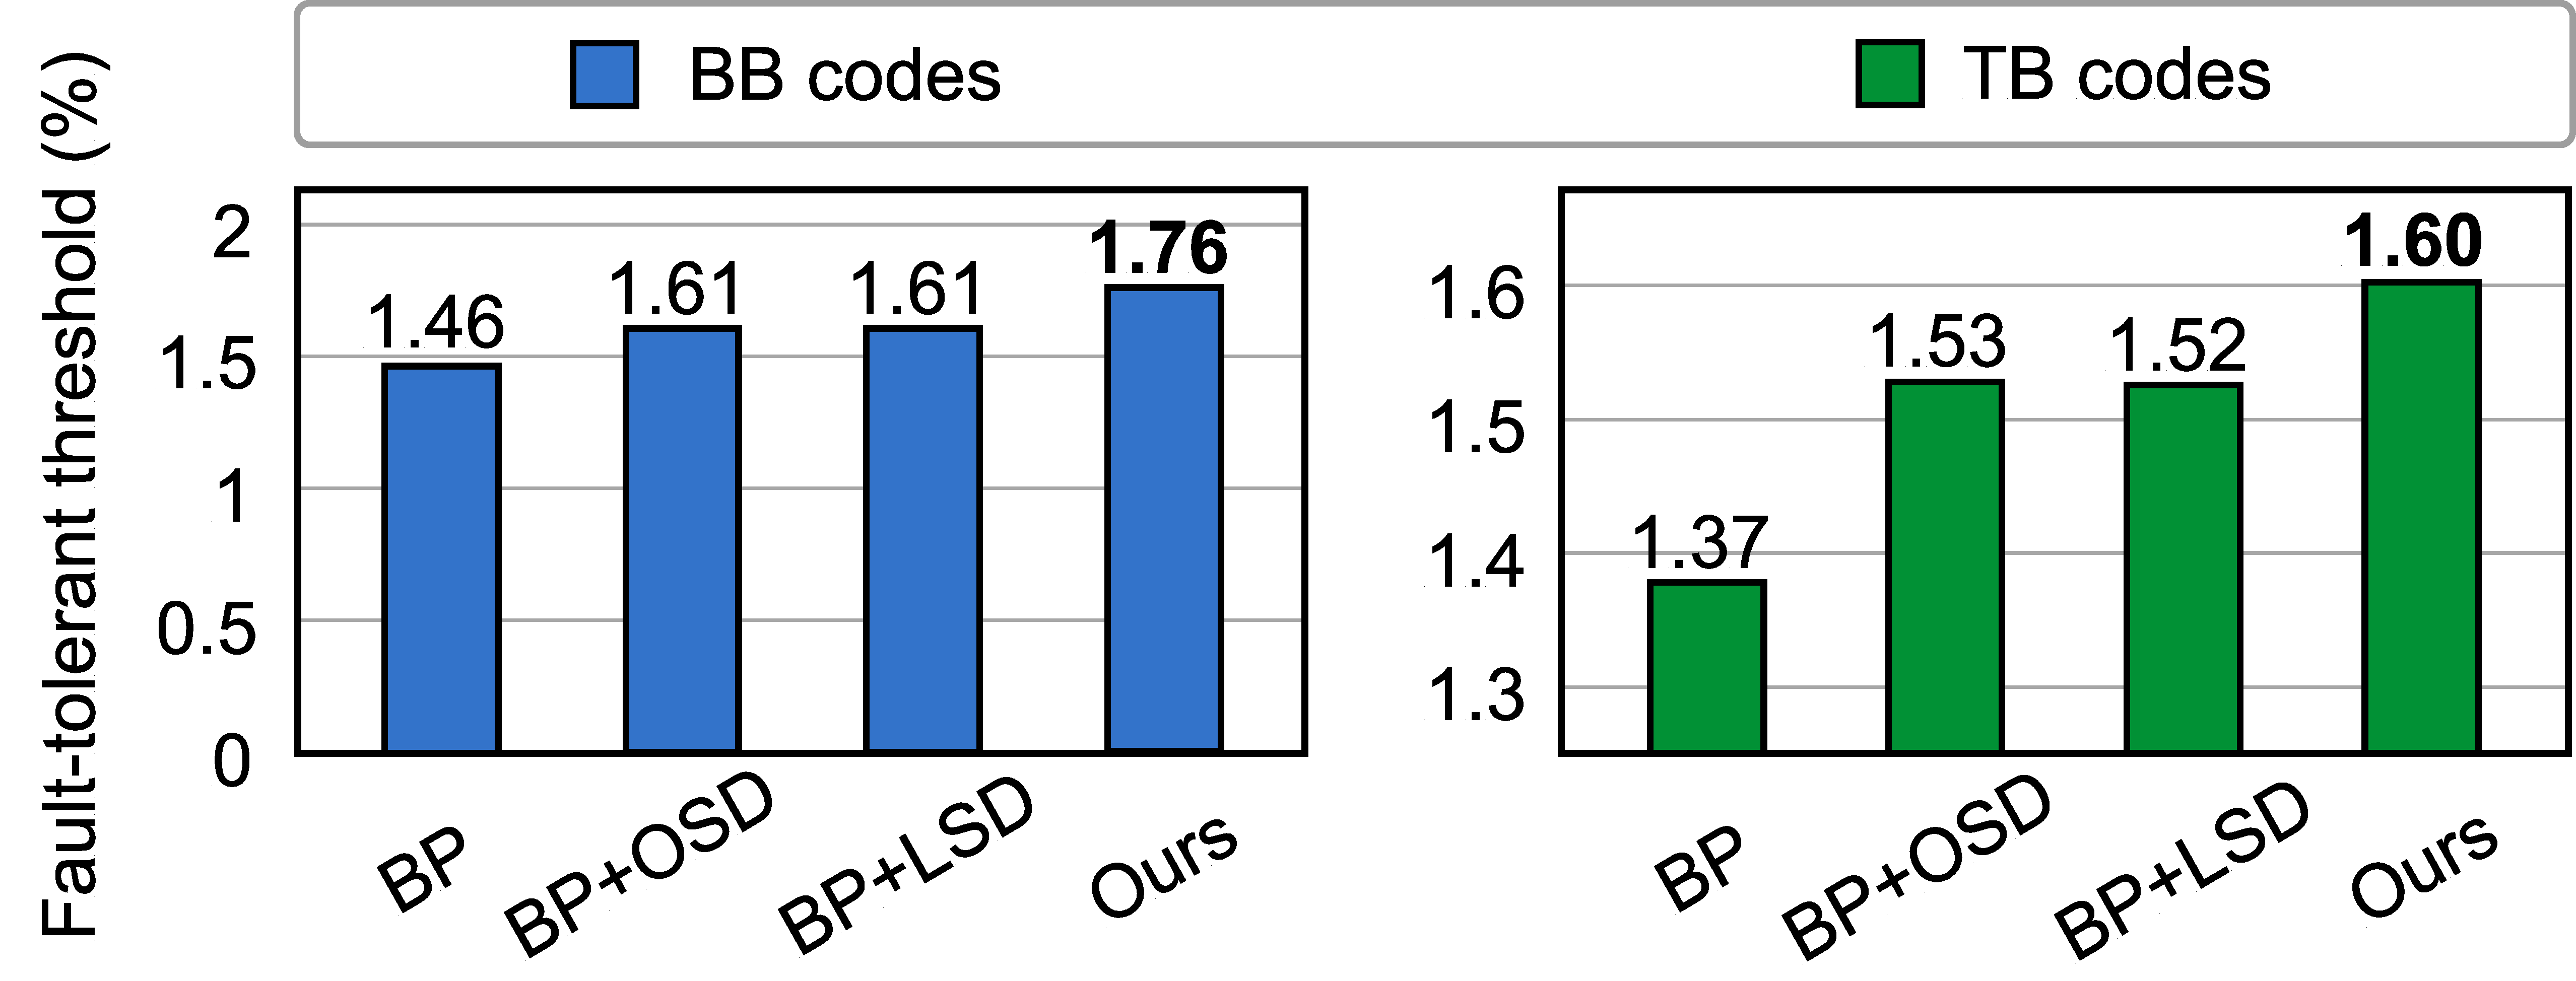
\includegraphics[width=1.0\columnwidth]{figures/Evaluation/fault_tolerant_threshold.pdf}}
% \vspace{-0.2cm}
% \caption{Fault-tolerant thresholds of BP \cite{bp}, BP+OSD \cite{bposd}, BP+LSD \cite{bplsd}, and \papername, respectively.}
% \vspace{-0.2cm}
% \label{fig:fault_tolerant_thresold}
% \end{figure}

% \textbf{Fault-tolerant threshold}.
% We calculate the fault-tolerant threshold of different decoders in different code types using the data in \autoref{fig:LER_exp}. The fault-tolerant thresholds are shown in \autoref{fig:fault_tolerant_thresold}. \papername outperforms other decoders in both BB codes and TB codes with thresholds of $1.76\%$ and $1.60\%$, respectively. The thresholds of BP+OSD and BP+LSD are similar and lower than \papername by $0.15\%$ and $0.08\%$ in BB codes and TB codes, respectively. BP has the lowest performance, which is lower than  \papername by $0.30\%$ and $0.23\%$. The high fault-tolerant threshold of \papername means that it has a higher fault-tolerance ability compared with other minimum weight decoders. \papername also improves the deployability of qLDPC codes on quantum hardware, since reducing the physical error rate in hardware takes much more effort than designing better codes. Notice that the higher fault-tolerant threshold does not imply higher logical error rates. Around the fault-tolerant threshold, the logical error rate of \papername is still lower than that of other decoders.



\subsection{Decoding Performance}

\textbf{Decoding latency}.
\autoref{fig:latency} plots the average decoding latency of different decoders. Latency of \papername ranges from $447\sim 1599 \mu s$, which is $3.37\times$ lower than the BP+OSD decoder on average. BP and BP+LSD have a lower latency than \papername since they leverage the message passing parallelism and localised statistics to accelerate decoding. Considering the excellent decoding accuracy of \papername, the longer latency than BP and BP+LSD is acceptable. Additionally, the latency growth of \papername over code size exhibits a linear trend, as \papername employs parallel marginal probability calculation to enhance parallelism in the decoding process. The complexity of \papername is linear with the number of logical qubits and syndrome qubits.

% Required packages:
% \usepackage{multirow}
% \usepackage{makecell}
% \usepackage{booktabs}

\begin{table}[t]
\centering
\renewcommand{\arraystretch}{1.25}
\caption{Tensor Compression of \papername.}
\label{tab:exp_tensor_compression}
\resizebox{\linewidth}{!}{
\begin{tabular}{c|l|lll|lll}
\toprule
\multirow{2}{*}{}& \makecell[l]{\textbf{Code}\\\textbf{type}}  &
\multicolumn{3}{c|}{\textbf{BB codes}} & \multicolumn{3}{c}{\textbf{TB codes}}  \\ \cline{2-8}
 & \makecell[l]{\textbf{Code}\\\textbf{size}} &
18 & 60 & 72 & 25 & 30 & 48 \\ \hline
% \midrule

% ================= COMPUTATION WORKLOAD ===================
\multirow{3}{*}{
\rotatebox{90}{%
    \parbox[c][.1cm][c]{2cm}{%
      \centering \textbf{FLOPS}%
    }%
  }%
}
 & \makecell[l]{{Exact}\\{MLD}}&
8.9K & 2.4G & 6.1T & $6.2$P & $10^3$P & $10^7$P \\ \cline{2-8}

 & \makecell[l]{Tensor\\MLD} &
640 & 5.6K & 49K & 320 & 2.0K & 131K \\ \cline{2-8}

 & \makecell[l]{Reduc-\\tion($\times$)} &
$14.2$ &
$10^{5}$ &
% $4.2\times10^{5}$ &

$10^{8}$ &
% $1.3\times10^{8}$ &

$10^{13}$ &
% $1.9\times10^{13}$ &
$10^{15}$ &
% $3.4\times10^{15}$ &
% $1.1\times10^{17}$
$10^{17}$
\\ \hline



% ================= NUMBER OF TENSORS ===================
\multirow{3}{*}{
\rotatebox{90}{%
\parbox[c][.1cm][c]{2cm}{%
      \centering \textbf{\#Tensor}%
    }%
    }
}
 & \makecell[l]{{Exact}\\{MLD}} &
40 & 128 & 156 & 52 & 63 & 102 \\ \cline{2-8}

 & \makecell[l]{Tensor\\MLD} &
11 & 34 & 42 & 14 & 15 & 26 \\  \cline{2-8}

 & \makecell[l]{Reduc-\\tion($\times$)} &
3.6& 3.8& 3.7&
3.7& 4.2& 3.9\\  \hline

% ================= MAX TENSOR SIZE ===================
\multirow{3}{*}{\rotatebox{90}{\makecell[c]{\textbf{Max tensor} \\\textbf{size}}}}
 & \makecell[l]{{Exact}\\{MLD}} &
4.0K & 0.1M & 0.5M & 8.1K & 0.2M & 1.0M \\ \cline{2-8}

 & \makecell[l]{Tensor\\MLD} &
512 & 512 & 512 & 512 & 512 & 512 \\ \cline{2-8}

 & \makecell[l]{Reduc-\\tion($\times$)} &
8& 256& 1024&
16& 512& 2048\\\hline
\multirow{4}{*}{
\rotatebox{90}{%
\parbox[c][.1cm][c]{2cm}{%
      \centering \textbf{Memory Footprint}%
    }%
    }
}
 & \makecell[l]{\textbf{Code}\\\textbf{size}} & 108      & 144      & 288      & 126      & 180      & 254      \\  \cline{2-8}

%  & \makecell[l]{\textbf{Code}\\\textbf{size}} &
% 18 & 60 & 72 & 25 & 30 & 48 \\ \hline

 & \makecell[l]{{Exact}\\{MLD}}  & 20KB    & 54KB    & 2.6MB  & 1.3MB  & 39MB & 3.9GB \\ \cline{2-8}
 & \makecell[l]{Tensor\\MLD}    & 1.1KB     & 1.4KB     & 2.8KB     & 4.0KB     & 6.0KB     & 8.7KB     \\ \cline{2-8}
 & \makecell[l]{Reduc-\\tion($\times$)}  & 18.2 & 36.7 & 914.5 & 333.3 & 6462 & 450176 \\
\bottomrule
\end{tabular}
}
\end{table}









% \begin{table*}[t]
% \centering
% \renewcommand{\arraystretch}{1.25}
% \caption{Tensor Compression of \papername.}
% \label{tab:exp_tensor_compression_transposed}

% % \resizebox{\textwidth}{!}{
% \begin{tabular}{
% l c
% |ccc
% |ccc
% |ccc
% }
% \toprule
% \textbf{Code type} &
% \makecell[c]{\textbf{Code}\\\textbf{size}} &
% \multicolumn{3}{c|}{\textbf{FLOPS}} &
% \multicolumn{3}{c|}{\textbf{\#Tensor}} &
% \multicolumn{3}{c}{\textbf{Max tensor size}} \\ \cline{3-11}
%  & & Exact & Tensor & Red. ($\times$) & Exact & Tensor & Red. ($\times$) & Exact & Tensor & Red. ($\times$) \\
% \midrule

% \multirow{3}{*}{BB codes}
%  & 18 &
% 8.9K & 640 & 14.2 &
% 40 & 11 & 3.6 &
% 4.0K & 512 & 8 \\ \cline{2-11}

%  & 60 &
% 2.4G & 5.6K & $10^{5}$ &
% 128 & 34 & 3.8 &
% 0.1M & 512 & 256 \\ \cline{2-11}

%  & 72 &
% 6.1T & 49K & $10^{8}$ &
% 156 & 42 & 3.7 &
% 0.5M & 512 & 1024 \\ 
% \midrule

% \multirow{3}{*}{TB codes}
%  & 25 &
% 6.2P & 320 & $10^{13}$ &
% 52 & 14 & 3.7 &
% 8.1K & 512 & 16 \\ \cline{2-11}

%  & 30 &
% $10^{3}$P & 2.0K & $10^{15}$ &
% 63 & 15 & 4.2 &
% 0.2M & 512 & 512 \\ \cline{2-11}

%  & 48 &
% $10^{7}$P & 131K & $10^{17}$ &
% 102 & 26 & 3.9 &
% 1.0M & 512 & 2048 \\

% \bottomrule
% \end{tabular}
% % }
% \end{table*}


\textbf{Tensor compression}. \autoref{tab:exp_tensor_compression} quantifies the complexity-accuracy tradeoff of \papername, highlighting the effectiveness of our tensor decomposition and compression. The results demonstrate a super-exponential reduction in computational workload (FLOPS) compared to Exact MLD. For instance, for the BB code [72,12,6]], \papername reduces the workload from 6.1 TFLOPS to just 49 KFLOPS. This advantage scales dramatically, achieving a $10^{17}\times$ reduction for the TB code [[48,4,8]].
In addition to computational gains, \papername significantly reduces memory requirements. The total number of tensors (\#Tensor) is consistently reduced by a factor of $3.6\times \sim 4.2\times$ across all codes. More critically, the Max Tensor Size, which represents the primary memory bottleneck, is shrunk from an exponentially growing value (e.g., 1.0M for the TB code [[48,4,8]]) to a small, constant 512. Considering this massive reduction in both computation and memory with little accuracy loss, \papername proves to be a highly efficient and scalable solution.





\subsection{Ablation Study}

In this section, we study the memory and computation cost of using different optimization techniques. We measure three different tensor network states, including the full tensor network without any
optimization, the matrix product state (MPS) with exact decomposition, and a 1D-chain matrix product state with offline contraction optimization. The metrics include storage memory for storing the tensor network, the Number of Floating Operations needed for tensor network contraction, and the Maximum Tensor Size when contracting the tensor network.

\textbf{Memory footprint.}
\autoref{fig:ablation_study}~(a)  shows the memory requirements for different tensor network states. After exact decomposition and offline contraction, 1D-chain MPS saves an average $9.1\times$ memory usage compared with the full tensor network, which consumes $5.2$KB memory on average. This trend is expected because the full tensor network, in its unoptimized form, represents a high-rank tensor whose memory consumption can be exponential in the worst case, whereas the 1D-chain MPS uses linear amounts of low-rank tensors.
We also find that only the MPS with exact decomposition has an average $39.1$KB memory usage, which is higher than the full tensor network. 
% This is because the exact decomposition decomposes the high-rank tensor with low-rank MPS, thereby increasing the number of tensors. Since the dimension $n$ of the original tensor equals the column sparsity of the check matrix, which is small in qLDPC codes, the reduction from $O(2^n)$ to $O(8n)$ is not remarkable.


\textbf{Number of floating operations.}
\autoref{fig:ablation_study}~(b) illustrates the number of floating operations required for tensor network contraction. The full tensor network demands $2.3\times10^{21}$  FLOPs, representing the highest computational burden. This contrasts sharply with MPS (with exact decomposition), which requires an average $8.0\times10^8$ FLOPs, and the 1D-chain matrix product state further reduces the computation cost to $3.1\times 10^4$ FLOPs, which is $7.3\times 10^{16}$ lower than the full tensor network. 
% The significantly higher FLOPs for the full tensor network stem from its inherently exponential worst-case computation complexity and the NP-hard problem of finding an optimal contraction path. 
The MPS offers theoretical polynomial-time complexity for contraction, drastically improving efficiency. The 1D-chain MPS with offline optimization further optimizes this for online decoding, explicitly leveraging a \textit{partial tracing strategy} with a polynomial complexity O($M\chi^2+\log K\cdot K^2\chi^4$), which is notably efficient compared to enumerating all logical spins. This can be observed from the reduction times compared with the full tensor network. The 1D-chain MPS achieves a $14.2\times$ reduction on the BB code [[18,4,4]] and a $1.3\times 10^8 \times$ reduction on the BB code [[2,12,6]], which depicts an exponential reduction trend.

\begin{figure}[t]
\centerline{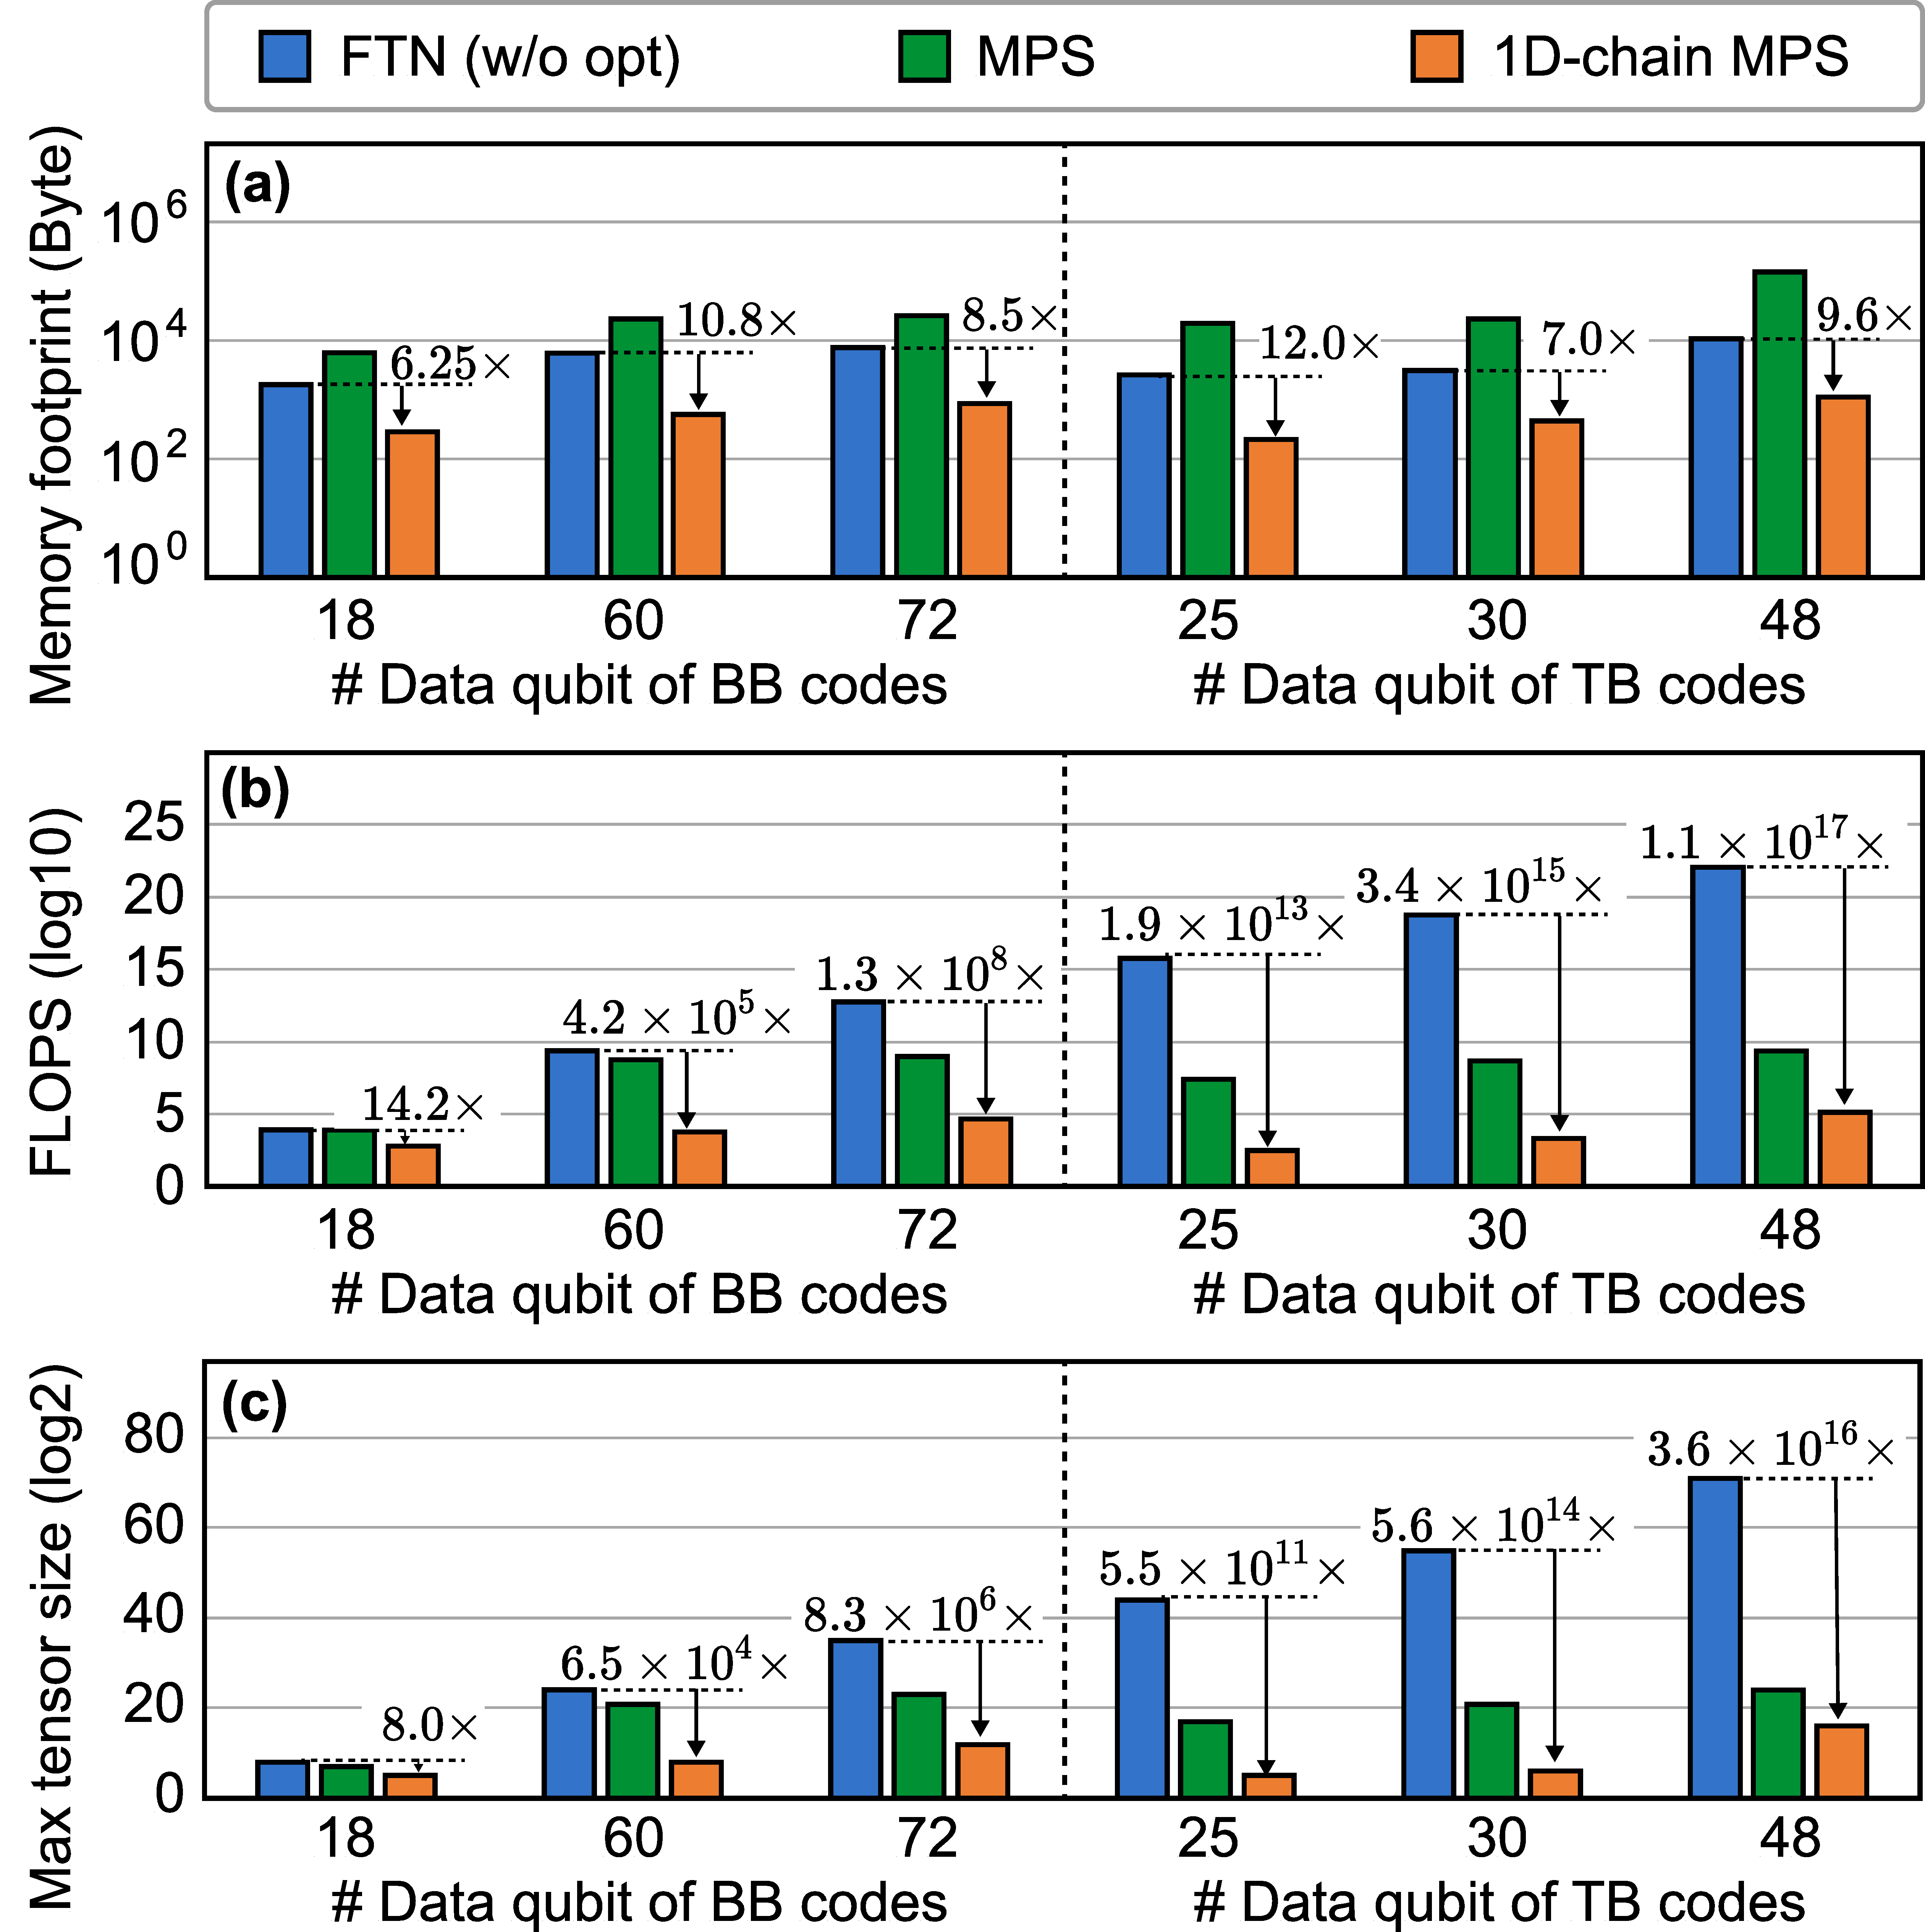
\includegraphics[width=1.0\columnwidth]{figures/Evaluation/ablation_study.pdf}}
\vspace{-0.3cm}
\caption{Ablation study of \papername.}
\vspace{-0.4cm}
\label{fig:ablation_study}
\end{figure}

\textbf{Maximum tensor size in computation.}
\autoref{fig:ablation_study}~(c) presents the maximum tensor size encountered during the contraction process. 1D-chain MPS achieves an $8\sim3.6\times 10^{16} \times$ reduction on maximum tensor size. The large maximum tensor size in the full tensor network is a direct consequence of the exponential growth of intermediate tensors during contraction. The peak tensor size, such as $2^{71}$ in TB code [[48,4,8]], often poses a memory bottleneck. The MPS fundamentally solves this by bounding intermediate tensor sizes, leading to a more manageable memory footprint in the contraction process. We can see that the maximum tensor size of a 1D-chain is always lower than $2^{20}$, which is a much lower memory than can be handled on classical devices.
\section{Related Works}
In this section, we provide an introduction to existing qLDPC decoders, most of which are developed based on the computational paradigms of belief propagation (BP) \cite{bp} or BP with ordered statistics decoding (BP+OSD) \cite{bposd}.

\subsection{BP-based qLDPC Decoders}
BP is a message-passing algorithm widely used in decoding qLDPC codes due to its linear-time complexity and suitability for sparse graph structures \cite{muller2025improved,miao2024joint}. However, standard BP suffers from low decoding accuracy due to its inability to fully account for quantum degeneracy and the presence of short cycles in the Tanner graph \cite{kuo2022exploiting}. To tackle this problem, numerous BP-based improved decoders have been proposed, such as enhanced feedback iterative decoding \cite{wang2012enhanced}, neural BP \cite{liu2019neural}, GF(2)-based augmented decoder \cite{rigby2019modified}, enhanced BP with trapping set dynamics \cite{chytas2024enhanced}. Recently, BP guided decimation (BP+GD) \cite{bpgd} has been proposed to encourage convergence by decimating the most reliable variable node in each iteration. Although these variants achieve higher accuracy than standard BP, their decoding performance still falls significantly short of that of maximum likelihood decoding (MLD) \cite{mld}, which remains the gold standard in terms of accuracy.

\subsection{Post-processing-based qLDPC Decoders}
In addition to BP-based improvements, some approaches enhance decoding accuracy through post-processing techniques, among which OSD is the most representative \cite{ninkovic2024decoding,bhattacharyya2025decoding}. However, OSD relies on computationally intensive operations, such as matrix inversion, which results in high decoding latency \cite{valls2021syndrome}. To solve this problem, BP+GDG \cite{bpgdg} proposes a sliding window decoder based on BP with guided decimation in the presence of circuit-level noise. Ambiguity clustering decoder \cite{wolanski2024ambiguity} divides the syndrome data into clusters that can be decoded independently, and decoders 144-qubit Gross code in 135$\mu s$ per round of syndrome extraction. Recently, BP+LSD \cite{bplsd} introduces a reliability-guided inversion decoder, which employs a parallel matrix factorization strategy to solve local decoding regions on the decoding graph. Although these methods improve scalability to some extent, they still involve matrix inversion operations, making it difficult to extend them to large-scale decoding problems.
\section{Discussion}

Currently, although the current GPU implementation does not yet meet the real-time decoding requirement of superconducting platforms, our accelerator design (e.g., tensor update unit and uncertain-bit detector) is well-suited for FPGA or ASIC customization. These units exhibit fixed dataflow patterns and deterministic parallelism, enabling pipelined designs that run at 500 MHz FPGA with reduced latency. After FPGA prototyping, these modules can be further fabricated as ASIC accelerators operating at speeds near 2 GHz, providing a two orders of magnitude improvement in decoding latency. On the other hand, we already satisfy the latency constraints of neutral-atom and ion-trap systems ($\sim 10^2 \mu s$) \cite{wolanski2024ambiguity}. Given that qLDPC codes require long-range connectivity, future qLDPC hardware is likely to be built on neutral-atom platforms \cite{pecorari2025high}. In this case, our decoder can offer both high precision and real-time performance. 

Regarding decoding accuracy, we compared \papername with exact MLD only on very small code (i.e., BB code [[18,4,4]]) because the computational cost of MLD grows exponentially with code size. Even high-performance GPUs (e.g., NVIDIA H100 with 80 GB memory) cannot evaluate medium-sized qLDPC codes with exact MLD due to the limited memory. On BB code [[18,4,4]], \papername achieves an average logical error rate ($3.3\times10^{-4}$) comparable to that of MLD ($3.1\times10^{-4}$), which enables higher noise levels in the future design of large-scale quantum chips. Moreover, higher decoding accuracy also helps relax the qubit connectivity requirements, making the chip less sensitive to underlying hardware constraints \cite{cao2025exact,chubb2021statistical}.

% Looking forward, several stages of the pipeline can benefit from FPGA-based design. For example, the tensor update path in the TCE can be mapped to a fully pipelined contraction unit with a scratchpad hierarchy, removing the general-purpose overheads of tensor cores. Likewise, the uncertain-bit detector of UDE matches FPGA spatial parallelism: each PE can be implemented as a hardwired datapath with fixed matrix selection and reduction logic, enabling deterministic per-bit processing. In addition, a lightweight FPGA control engine can orchestrate refinement rounds without GPU scheduling overhead. With these customized modules, the end-to-end latency can be reduced substantially. For instance, a GPU-bound latency on the order of $10^3 \mu s$ can be decreased to sub-$10^1 \mu s$, yielding both higher throughput and better energy efficiency than a pure GPU design.
\section{Conclusion}
% In this paper, we propose a maximum likelihood decoder for CSS qLDPC codes via the tensor network. We formulate the calculation of the logical error rate into the free energy of the spin-glass model and leverage the tensor network to compute the free energy. We further provide the exact matrix product state representation and use an offline contraction strategy to reduce the connection dimension to a 1D chain. The 1D-chain matrix product state can be contracted in polynomial time, which is used for online decoding. We also develop a conditional marginal probability calculation method for finding the most likely logical error online, which has a polynomial complexity related to the number of logical qubits.

In this paper, we propose a tensor-network-based maximum likelihood decoder for CSS qLDPC codes. By mapping logical error estimation to the free energy of a spin-glass model, we leverage tensor networks for efficient computation. We construct an exact matrix product state representation and apply an offline contraction to reduce the network to a 1D chain, enabling polynomial-time online decoding. A conditional marginal probability method is further developed to identify the most probable logical error with polynomial complexity in the number of logical qubits.

\section*{Appendix}~\label{sec:appendix}
% \subsection{Proof of Lemma~\ref{theorem:decodingTensor}}
In this appendix, we give the brief proof of Lemma~\ref{theorem:decodingTensor} and see~\url{https://arxiv.org/pdf/xxxx.xxxx} for a detailed proof. This proof consists of three steps: representing logical probability via stabilizer subspace shifting, converting the probability calculation into a spin glass model, and calculating the spin glass model via tensor networks.

% The maximum likelihood decoding for qLDPC codes centers on finding the most 
% likely logical syndrome \( \vec{s}_L \) given an observed syndrome \( \vec{s} \), governed by the relationship:

% \[
% \begin{bmatrix}
% H_x \\ L_x
% \end{bmatrix} \vec{e_z} = \begin{bmatrix}
% \vec{s} \\ \vec{s}_L
% \end{bmatrix} \mod 2
% \]
% Here, we use $Z$-type errors $\vec{e_z}$ for illustration, where each error \( e_j \in \{0,1\} \) having prior probability \( p_j \).  \( H_x\) is the check matrix, \( L_x \) is the logical check matrix where each row is a logical $X$-operator, \( \vec{s} \) is the observed syndrome, and \( \vec{s}_L \) is the logical syndrome representing the logical error. The maximum likelihood decoding goal is to maximize:
% \begin{equation}\small
% \vec{s}_L = \arg\max_{\vec{s_L}} \sum_{\{\vec{e} \mid 
% H_x \vec{e_z} = \vec{s}, L_x \vec{e_z}  =\vec{s}_L \}} P(\vec{e}) \label{eq:logicalsyndrome}
% \end{equation}
\subsection{Logical Probability Representation through Stabilizer Subspace Shifting}\label{subsec:proofA}
Without loss of generality, here we consider decoding the $Z$-type error. Leveraging the relationship between destabilizers, stabilizers, and logical operators, we can further prove that this probability can be represented by 
\begin{equation}\label{eq:logicalstab}
    P(\vec{l}|\vec{s}) =  \textstyle  \sum_{\vec{z} \in \{0,1\}^M} P(H_{\text{des}}^T \vec{s} \oplus H_z^T \vec{z} \oplus L_z^T \vec{l})
\end{equation}

Where $H_{\text{des}}$ is the destabilizer matrix with each row an x-destabilizer. \( H_z\) is the $Z$-type check matrix, where each row is an x-stabilizer, \( L_z \) is the $Z$-type logical matrix where each row is a logical $z$-operator.
% For a decoding problem, the probability of an error vector $\vec{e}$ is 
% \begin{equation}
% \small
% P(\vec{e}) = e^{-\sum_{j=1}^n 2w_j e_j}, \quad w_j = \ln \left( (1 - p_j)/p_j \right) /2 \notag
% \end{equation}
% where \( P(\vec{e})  \) is the physical error probability and $p_j$ is the phyiscal probability of occuring error $e_j=1$.



% For $X$-type error, the error vector in $Z$-stabilizer space \( H_z^T \vec{z}, \vec{z} \in \{0,1\}^M \) has zero syndrome and zero logical error since the $Z$-check matrix $H_z^T$ is the kernel space of $H_x$ and $L_x$. The logical-$Z$ operator space \( L_z^T \vec{l} , \vec{l} \in \{0,1\}^K \) has zero syndrome but a nonzero logical error.  
% And we can prove that these two subspaces form the full $X$-type error space with zero syndrome. For given syndrome $\vec{s}$, we can get an initial error that has the syndrome $\vec{s}$ by \( H_{\text{des}}^T \vec{s} \) from the destabilizer matrix \( H_{\text{des}} \). Then we can express the error space as
% \begin{equation} \small
%     \vec{e}_x=\underbrace{\quad H_z^T  \vec{z} \quad}_{\text{stabilizer subspace}} \oplus \underbrace{ \quad L_z^T \vec{l} \quad}_{\text{logical shifting}} \oplus \underbrace{\quad H_{\text{des}}^T  \vec{s} \quad}_{\text{syndrome shifting}} \label{eq:error}
% \end{equation}
% It is easy to verify that all errors $\vec{e} $ are consistent with the syndrome $\vec{s}$ since the $Z$-stabilizer space and logical-$Z$ operator space have zero syndrome. Furthermore, since the logical-$Z$ operator space has the same rank as the logical operator, the errors $\vec{e}$ under the same $\vec{l}$ must belong to the same logical $X$ error $\vec{s}_L$.
 % We can transform the decoding problem into:

% After finding the optimal $\vec{l}^*$, the detected logical operator for correction is
% \begin{equation} \small
%     \vec{e}^* = H_{\text{des}}^T \vec{s} \oplus L_z^T \vec{l}^* \label{eq:recovererror}
% \end{equation}
% This unconstrained formulation simplifies the summation by parameterizing errors over stabilizer and logical operators.

\subsection{Express Logical Probability in Spin Glass Model}\label{subsec:proofB}

To handle the summation over \( \vec{z} \), we map the problem to a spin glass model, inspired by statistical mechanics~\cite{cao2025exact,sourlas1989spin}. We transform bits into spins: \( \epsilon_j = (-1)^{e_j} \), so \( e_j = (1 - \epsilon_j)/2 \). Under this transformation, the logical error probability in \autoref{eq:logicalstab} becomes:
% \[\small
% P(\vec{e}) = C \exp \left( \sum_{j=1}^n \omega_j \epsilon_j \right),  C = \exp(\sum_{j=1} w_j)
% \]
% where \( C \) is a normalization constant. Substituting \( \vec{e} \) with \autoref{eq:error} and use the spin representation $\vec{y},\vec{t},\vec{g}$ for bits $\vec{s},\vec{z},\vec{l}$ we can represent the error probability as
\begin{equation} \small \label{eq:logicalprobH}
    P(\vec{l}|\vec{s}) = C\exp \left( - H \right), C = \exp(\sum_{j=1} w_j)
\end{equation}
\begin{equation} \small\label{eq:hamiltonian}
    {\tiny  H }= { \tiny -\sum_{j=1}^n \omega_j\prod_{\{k|H_{des}(k,j)\neq 0\}} y_k \prod_{\{k|H_{z}(k,j)\neq 0\}} t_k \prod_{\{k|L_z(k,j)\neq 0\}} g_k }
\end{equation}
Here, $H$ is the Hamiltonian of this spin glass system. Each energy term in the Hamiltonian is determined by the spins. 

\subsection{Calculating Spin Glass Model via Tensor Network}\label{subsec:proofC}
Since the summation term in the exponent is equivalent to the continuous multiplication of exponential terms, \eqref{eq:logicalprobH} and \eqref{eq:hamiltonian} can be written as
\begin{equation}\small
    P(\vec{l}|\vec{s}) = C\prod_j \exp \left (\omega_j \prod y_k \prod t_k \prod g_k \right )
\end{equation}
For the constraint part, we use the Kronecker tensor to represent it, so the formula transforms into contraction tensor network with a Tanner graph connection. Then, we can convert the summation into a contraction of the tensor network. 
\begin{equation} \small
    P(\vec{l}|\vec{s}) = \frac{{\text{contract}}(\mathcal{T}(\vec{l},\vec{s}))}{\text{contract}(\mathcal{T}(\vec{s}))}. 
\end{equation}


% \section*{Appendix}
% \begin{algorithm}[t]
\caption{Online Decoding via Conditional Marginal Probability}
\label{alg:conditional-decoding}
\SetKwFunction{Pjudge}{JudgeP}
\SetKwFunction{Contract}{Contract}
\SetKwProg{Fn}{Function}{:}{end}

\KwIn{Measured syndrome vector $\boldsymbol{s} = (s_1, \dots, s_M)$; 
MPS chain with tensor set $\mathcal{T} = \{\mathcal{T}_1, \dots, \mathcal{T}_{M+K}\}$ with maximum bond $\chi$. Each tensor has shape [$\chi$,$\chi$,2]. Here, M is the length of syndrome bits, and K is the length of logical bits.} 
\KwOut{Decoded logical spin vector $\boldsymbol{l} = (l_1, \dots, l_K)$.}



\Fn{\Pjudge{$P$}}{
    \If{$P > 0.6$}{\KwRet  $1$}
    \If{$P < 0.4$}{\KwRet $0$}{
            \KwRet $\text{unknown}$
        }
}
\Fn{\Contract{$\{\mathcal{A}_1, \dots, \mathcal{A}_{T}\}$}}{
    \For{$p = 1 \dots \log_2 T$}{
        \ForPar{$i = 1 \dots \frac{T}{2^p}$}{
        $\mathcal{A}_{2i}[:][:] \leftarrow 
        \sum_{t=0}^{\chi-1} \mathcal{A}_{2i}[:][t]\times \mathcal{A}_{2i+1}[t][:]$  \tcp*[r]{Matrix-matrix product}
        pop $\mathcal{A}_{2i+1}$ from chain $\mathcal{A}$;
        }
    }
    \KwRet $\mathcal{A}_{0}$
}


% =========================================================
\textbf{Step 1: Fix syndrome indices and contract to logical MPS}\\
\ForPar{$i = 1 \dots M$}{
    \tcp{Fix physical index of $\mathcal{T}_i$ by measured $s_i$}
    $\mathcal{T}_i[:][:] \leftarrow \mathcal{T}_i[:][:][s_i]$
}

\tcp{Multiply the M matrices in tree}
% \For{$p = 1 \dots \log_2 M$}{
%     \ForPar{$i = 1 \dots \frac{M}{2^p}$}{
%     $\mathcal{T}_{2i}[:][:] \leftarrow 
%     \sum_{t=1}^{\chi} \mathcal{T}_{2i}[:][t]\times \mathcal{T}_{2i+1}[t][:]$  \tcp*[r]{Matrix-matrix product}
%     pop $\mathcal{T}_{2i+1}$ from chain $\mathcal{T}$;
%     }
% }
$\mathcal{T}_{0} \gets $  \Contract{$\{\mathcal{T}_1, \dots, \mathcal{T}_{M}\}$}\;
$\mathcal{T}_{M+1}[:][:][0] \gets  \sum_{t=0}^{\chi-1}\mathcal{T}_{0}[:][t]  \times  \mathcal{T}_{M+1}$[t][:][0] \;
$\mathcal{T}_{M+1}[:][:][1] \gets  \sum_{t=0}^{\chi-1}\mathcal{T}_{0}[:][t]  \times  \mathcal{T}_{M+1}$[t][:][1] \;


\tcp{After Contraction, MPS chain has only K tensors.}



\end{algorithm}



\begin{algorithm}[t]
\caption{Online Decoding via Conditional Marginal Probability (Continue)}

% =========================================================
\BlankLine
\textbf{Step 2: Conditional refinement of uncertain bits} \\
\For{$i = 1 \dots K$}{
    $l_i \gets \text{unknown}$\; \tcp{Initialize logical bits }
}
\While{$\exists\; l_i \in \vec{l} == \text{unknown}$}{
    \ForPar{all unknown $i$}{
            \tcp{Contract locally with $l_i =0,1$}
            \For{$\lambda \in \{0,1\}$}{
                % $\psi_\lambda \leftarrow \text{Identity matrix with shape }[\chi, \chi]$ \tcp*[r]{Initialize scalar}
                \For{$k = 1 \dots K$}{
                    \If{$k=i$}{
                        $T_k'[:][:] \leftarrow \mathcal{T}_k[:][:][\lambda]$
                    }\If{$l_k \in \{0,1\}$}{
                    $\mathcal{T}_{k}'[:][:] \leftarrow \mathcal{T}_{k}[:][:][l_k]$
                }\Else{
                        $\mathcal{T}_k'[:][:] \leftarrow \mathcal{T}_k[:][:][0]+ \mathcal{T}_k[:][:][1]$
                    }
                    % $\psi_\lambda[:][:] \leftarrow \sum_{t=1}^\chi \psi_\lambda[:][t] \times T_k'[t][:]$ \tcp*[r]{Matrix-matrix product}
                }
                $\psi_\lambda[:][:] \leftarrow$ \Contract{$\{\mathcal{T}'_1, \dots, \mathcal{T}'_{K}\}$}
                
                $F_\lambda \leftarrow |\sum_{t=1}^{\chi} \psi_\lambda[t][t]|$
            }

            $P_i^{\text{cond}} \leftarrow \dfrac{F_{1}}{F_{1} + F_{0}}$ \;
            $l_i \leftarrow$ \Pjudge{$P_i$}
        
    }
}

\BlankLine
\Return{$\boldsymbol{l}$}

\BlankLine
\textbf{Complexity Summary:} \\
Sequential: $O(M\chi^2 + \log K \cdot K^2\chi^4)$; \\
Parallel: $O(M\chi^2 + \log K \cdot K\chi^4)$.

\end{algorithm}


% \section*{Acknowledgements}
% This document is an updated version of HPCA 2022 and 2023, which, in
% turn, has been derived from two previous conferences, in particular
% HPCA 2021 and MICRO 2021, which, in turn, are derived from past MICRO,
% HPCA, ISCA, and ASPLOS conferences.

%%%%%%% -- PAPER CONTENT ENDS -- %%%%%%%%


%%%%%%%%% -- BIB STYLE AND FILE -- %%%%%%%%
\bibliographystyle{IEEEtranS}
\bibliography{refs}
%%%%%%%%%%%%%%%%%%%%%%%%%%%%%%%%%%%%

\end{document}

